\documentclass[hidelinks,12pt]{article}

\usepackage[titletoc,toc,page]{appendix}
\usepackage{algorithm2e}
\usepackage[brazil]{babel}
\usepackage[utf8]{inputenc}
\usepackage{indentfirst}
\usepackage{caption}


\usepackage{hyperref}
\usepackage{fancyhdr}

\usepackage{listings}
\usepackage[export]{adjustbox}
\usepackage{xcolor}
\newcommand{\icon}[1]{\includegraphics[height=12pt]{#1}}
\newcommand{\bigicon}[1]{\includegraphics[height=50pt]{#1}}



\lstset{frame=tb,
	language=Java,
	aboveskip=3mm,
	belowskip=3mm,
	showstringspaces=false,
	columns=flexible,
	basicstyle={\small\ttfamily},
	numbers=none,
	numberstyle=\tiny\color{gray},
	keywordstyle=\color{blue},
	commentstyle=\color{dkgreen},
	stringstyle=\color{red},
	breaklines=true,
	breakatwhitespace=true,
	tabsize=3,
	numbers=left
}

\lstset{
	language=Python,
	basicstyle=\ttfamily,
	otherkeywords={self},             
	keywordstyle=\ttfamily\color{blue!90!black},
	keywords=[2]{True,False},
	keywords=[3]{ttk},
	keywordstyle={[2]\ttfamily\color{yellow!80!orange}},
	keywordstyle={[3]\ttfamily\color{red!80!orange}},
	emph={MyClass,__init__},          
	emphstyle=\ttfamily\color{red!80!black},    
	stringstyle=\color{green!80!black},
	showstringspaces=false,
	numbers=left           
}


\DeclareCaptionFont{white}{\color{white}}
\DeclareCaptionFormat{listing}{%
	\parbox{\textwidth}{\colorbox{gray}{\parbox{\textwidth}{#1#2#3}}\vskip-4pt}}
\captionsetup[lstlisting]{format=listing,labelfont=white,textfont=white}
\lstset{frame=lrb,xleftmargin=\fboxsep,xrightmargin=-\fboxsep}


\newcommand{\iconb}[1]{\includegraphics[height=20pt]{#1}}
\setcounter{secnumdepth}{5}

\fancypagestyle{plain}{%
	\fancyfoot{}%
	\fancyhead{}%
}


\begin{document}
\pagenumbering{gobble}
\pagestyle{fancy}


\lhead{\bigicon{Figures/ufu}}
\chead{{\footnotesize UNIVERSIDADE FEDERAL DE UBERLÂNDIA \\ FACULDADE DE CIÊNCIA DA COMPUTAÇÃO \\ Construção de Compiladores} \\ \scriptsize{Av. João Naves de Ávila 2121, Campus Santa Mônica} }
\rhead{\bigicon{Figures/facom}}
\lfoot{}
\cfoot{}
\rfoot{}
\vspace*{8.5cm}
\begin{figure}[!h]
	\centering
	\Huge{Relatório de Compiladores Python para Dalvik}
\end{figure}

\vspace{5cm}
\noindent\textbf{Alunos:}\\ Gabriel Augusto Marson - 11221BCC022  \\ Leonardo da Silva Martins - 11321BCC034\\
\textbf{E-mail:} gabrielmarson@live.com\\
\textbf{Profº.:} Alexsandro


\newpage
\fancyhead[C]{}
\fancyhead[R]{}
\fancyhead[L]{\leftmark}
\fancyfoot{}
\fancyfoot[L]{{\footnotesize  Construção de Compiladores}}
\fancyfoot[C]{\hspace{1.5cm}\thepage}
\fancyfoot[R]{{\footnotesize Python to Dalvik}}
\pagenumbering{arabic}


{\let\thefootnote\relax\footnotetext{\textit{UFU, Universidade Federal de Uberlândia, Minas Gerais, Brasil}}}

\newpage

\tableofcontents


\newpage

\section{Introdução}

	Esse relatório contém informações à respeito da instalação das tecnologias necessárias(Dalvik, OCaml, Python, etc) para o processo de contrução de compiladores. 
	Além disso, procurou-se extrair informações à respeito das regras que o compilador Dalvik usa para processar as linguagens.
	
\section{Configuração do Ambiente}

	Nesta seção, será apresentado uma breve descrição sobre as ferramentas que serão usadas e como configurá-las para o nosso experimento.

	\subsection{Ubuntu 16}
	
	Ubuntu é um sistema operacional com núcleo do linux. Pode-se baixá-lo no  \href{http://www.ubuntu.com/download}{\color{blue}site oficial} clicando em \textbf{Ubuntu Desktop}. A instalação pode ser feita via CD ou via boot pelo pendrive.
	
	Foi baixado e instalado o Ubuntu 16.04 LTS.
	
	\subsection{OCaml}
		
	Para instalar a linguagem OCaml no Ubuntu, basta digitar no terminal:\\
	
	\noindent\fbox{%
		\parbox{\textwidth}{%
			$>$ sudo apt-get install ocaml
		}%
	}\\
	
	A versão instalada do OCaml foi a 4.02.3.
	
	\subsection{Oracle Java JDK 8}
	
	É recomendado usar o o JDK para o desenvolvimento Android.
	Para simplificar o download e instalação, precisaremos adicionar um PPA(Personal Package Archive) via linha de comando:\\
	
	\noindent\fbox{%
		\parbox{\textwidth}{%
			$>$ sudo add-apt-repository ppa:webupd8team/java\\
			$>$ sudo apt-get update\\
			$>$ sudo apt-get install oracle-java8-installer
		}%
	}\\
	
	Para verificarmos se o JDK foi instalado com sucesso, basta digitarmos o comando \texttt{java -version}. A saída esperada é algo semelhante a isto:\\
	
	\noindent\fbox{%
		\parbox{\textwidth}{%
			java version "1.8.0\_101"\\
			Java(TM) SE Runtime Environment (build 1.8.0\_101-b13)\\
			Java HotSpot(TM) 64-Bit Server VM 
			(build 25.101-b13, mixed mode)
		}%
	}\\
	
	\subsection{Python}
	
	Criada por Guido van Rossum em 1991, Python é um linguagem de programação imperativa, orientada objetos e de tipagem dinâmica forte.
	O python já vem instalado no Ubuntu.
	A versão do Python utilizada foi a 3.5.2.
	
	\section{Android SDK}
	
	O Android SDK inclui ferramentas para que programadores consigam desenvolver as suas aplicações e, no caso desse trabalho, executar um código .smali. O download pode ser feito diretamente no \href{https://developer.android.com/studio/index.html#tos-header}{\color{blue}site}. Pode-se baixar o Android Studio ou somente o Android SDK. Optamos pelo SDK. 
	
	Após baixar o arquivo, descompacte-o, acesse a pasta tools e digite.\\
	
	\noindent\fbox{%
		\parbox{\textwidth}{%
			$>$ ./android
		}%
	}\\
	
	Será exibida uma janela com a opção de alguns arquivos default marcados para instalação. Clique no botão InstallPackages 
	\newpage
	\begin{figure}[h!]
		\centering
		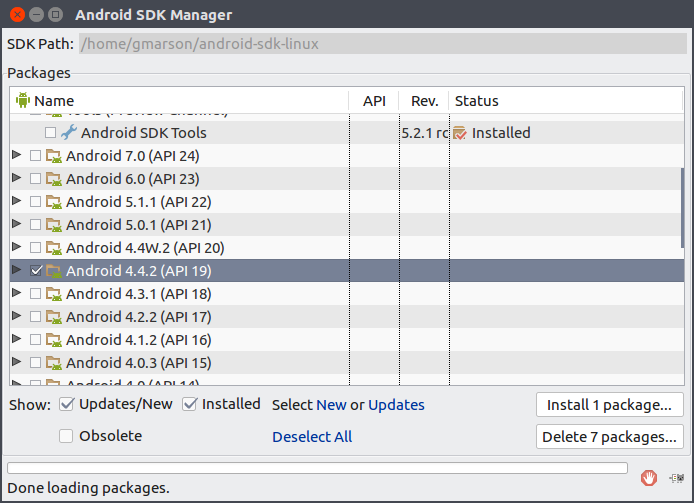
\includegraphics[scale=0.5]{Figures/SDKManager}
	\end{figure}
	
	Recomenda-se o download de todas as tools e qualquer API do android. No caso, foi baixada a API 19.
	
	\subsubsection{Configurando as variáveis de ambiente}
	
	
	
	Edite o arquivo \texttt{bashrc} e acrescente as linhas a seguir salvando o arquivo posteriormente.\\
	
	\begin{lstlisting}[caption=Variáveis android de ambiente,language=java]
	#Editando o bash
	gedit ~./bashrc
	
	#Android
	export PATH=${PATH}:~/android-sdk-linux/tools
	export PATH=${PATH}:~/android-sdk-linux/platform-tools
	export PATH=${PATH}:~/android-sdk-linux
	
	\end{lstlisting}
	
	
	
	Em seguida, basta recarregarmos o bash:\\
	
	\noindent\fbox{%
		\parbox{\textwidth}{%
			$>$ source ~/.bashrc
		}%
	}
	
	\subsubsection{Dispositivo Virtual Android}
	
	O dispositivo Virtual Android é um emulador usado para testes de aplicações. Um Android Virtual Device(AVD) é um emulador que permite replicar um dispositivo real, especificando opções de hardware e software. Será usado um AVD para que se possa executar uma máquina Dalvik. Pelo comando:\\
	
	\noindent\fbox{%
		\parbox{\textwidth}{%
			$>$ android list targets
		}%
	}\\
	
	É esperado que as APIs do android que foram baixadas aparecam listadas. Algo similar a esta imagem:\\
	
	\begin{figure}[h!]
		\centering
		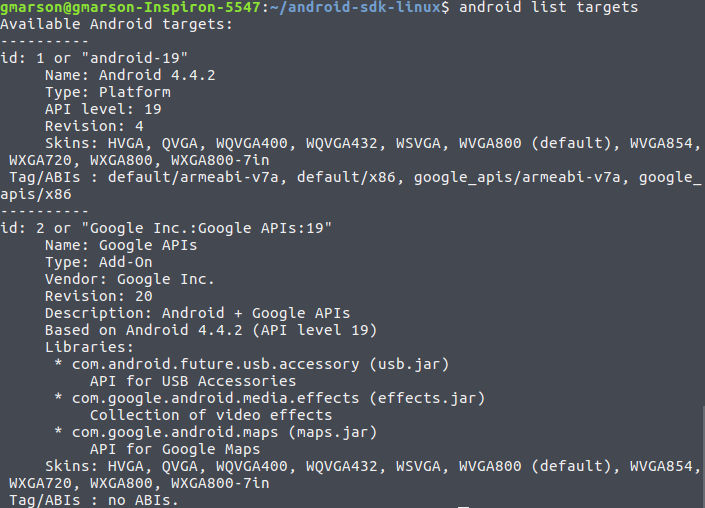
\includegraphics[scale=0.7]{Figures/listAndroid}
	\end{figure}
	
	\newpage
	\subsubsection{Criando um AVD}
	
	Para criar uma AVD, selecione um dos dispositivos previamente listados e digite o comando nesse formato:
	\texttt{android create avd -n < nomeDaMaquina > -t < APIMaquina  >}. Segue o exemplo:
	
	\begin{figure}[h!]
		\centering
		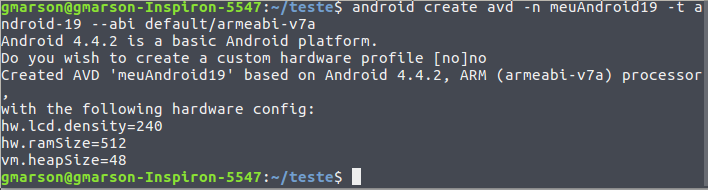
\includegraphics[scale=0.7]{Figures/createAVD}
	\end{figure}
	
	Seguem alguns comandos úteis:
	
	{\color{blue}{Ver}} : \texttt{emulator -avd meuAndroid19}
	
	{\color{red}{Deletar}} : \texttt{android delete avd -n meuAndroid19}	
	
	\section{Dalvik}
	
	Dalvik é uma máquina virtual criada para o sistema Android e que emula operações de CPU e compila códigos de uma linguagem fonte para um bytecode específico da máquina virtual. Otimizada para dispositivos móveis ou com hardware limitado, Dalvik foi projetada de modo a permitir a execução de várias instâncias ao mesmo tempo de forma eficaz.
	
	Por trás desta eficácia, escondem-se certas medidas que determinaram o bom funcionamento dessa VM(Virtual Machine). Dentre elas, convém mencionar o processo {\texttt{Zygote}} que é responsável pelo compartilhamento de código entre as instâncias de programa na Dalvik.
	
	 \subsection{Dalvik e JVM}
	 
	 A diferença entre Dalvik e JVM está no fato de que as duas possuem bytecodes diferentes.
	 Quando é criado um aplivativo java no computador, a JVM executa tudo o que foi compilado a partir do código fonte.
	 
	 \begin{figure}[!h]
	 	\centering
	 	
\includegraphics[scale=0.6]{Figures/java}
	 	\caption{Processo de Compilação em JVM}
	 \end{figure}
	
	Na máquina Dalvik o processo ocorre de forma similar. A diferença é que existe um compilador \texttt{dx} que pega os arquivos .class e os transforma para .dex. Esse último formato é processado pelo aapt(Android Packaging Tool) e convertido em um arquivo .apk .
	
	\begin{figure}[!h]
		\centering
		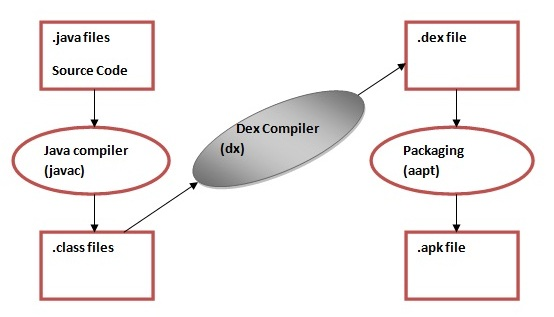
\includegraphics[scale=0.5]{Figures/dalvik-flow}
		\caption{Processo de Compilação Dalvik}
	\end{figure}
	
	
	
	\subsection{Smali/Backsmali}
	
	O assembler(programa que transforma um código Assembly, no caso, smali, para linguagem de máquina) da máquina virtual Dalvik é o Smali. O Backsmile é usado para converter um arquivo .dex em um código fonte .smali.
	
	O download dos dois pode ser feito via bitbucket:\\
	
	\noindent\fbox{%
		\parbox{\textwidth}{%
			$>$ cd
			
			$>$ mkdir Smali 
			
			$>$ cd Smali
			
			$>$ wget https://bitbucket.org/JesusFreke/smali/downloads/smali-2.1.3.jar
			
			$>$ wget https://bitbucket.org/JesusFreke/smali/downloads/baksmali-2.1.3.jar
		}%
	}\\	

	\subsection{Execução de um Programa na Dalvik}
	
	Para exemplificar o uso do smali, usaremos o seguinte código adquirido de [\ref{Alana}]:\\
	



\begin{lstlisting}[caption=Smali,language=java]
.class public LHelloWorld

.super Ljava/lang/Object;
.method public static main([Ljava/lang/String;)V
.registers 2
	sget-object v0, Ljava/lang/System;->out:Ljava/io/PrintStream;
	const-string	v1, "Hello World!"
	invoke-virtual {v0, v1}, Ljava/io/PrintStream;->println(Ljava/lang/String;)V
	return-void
.end method
\end{lstlisting}
	
	Deve-se primeiramente, salvar esse código no mesmo diretório em que estão o smali.jar e o backsmali.jar. Em seguida, digitaremos os seguintes códigos que são necessários para rodar esse programa na máquina android.\\

\noindent\fbox{%
	\parbox{\textwidth}{%
		$> $cd $\sim$/Dalvik
		
		$> $java -jar smali-2.0.3.jar -o classes.dex HelloWorld.smali
		
		$>$ zip HelloWorld.zip classes.dex
	}%
}\\		
	
	\textbf{É imperativo que o .dex gerado seja chamado de classes.dex}.
	Agora, deve-se ligar o emulador do android. Relembrando que AVD significa android virtual device.\\
	
	\noindent\fbox{%
		\parbox{\textwidth}{%
		$>$	emulator -avd meuAndroid19 \&
			
		}%
	}\\	

	Será usado o ADB(Android Debug Bridge) que é um comando versátil que permite a comunicação do sistema operacional com uma instância de emulador android. Esse comando diz para o SO colocar o arquivo HelloWorld.zip dentro do meuAndroid19.\\
	
	\noindent\fbox{%
		\parbox{\textwidth}{%
			$>$ adb push HelloWorld.zip /data/local
			
		}%
	}\\	
	
	Em seguida, basta executarmos:\\
	
	\noindent\fbox{%
		\parbox{\textwidth}{%
			$>$ adb shell
			
			$>$ dalvikvm -cp /data/local/HelloWorld.zip HelloWorld
			
		}%
	}\\
	
	Esse comando executa a dalvikVM no arquivo HelloWorld.zip
	
	A saída esperada é:
	
	\begin{figure}[!h]
		\centering
		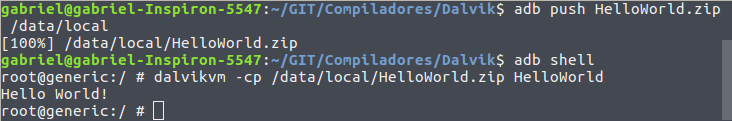
\includegraphics[scale=0.5]{Figures/smaliOutput}
	\end{figure}
	
	Para fecharmos a emulação do Android, basta digitarmos o comando:\\
	
	
	\noindent\fbox{%
		\parbox{\textwidth}{%
			$>$ adb emu kill
			
		}%
	}\\
	
	


\section{Análise do comportamento de compilação de .java para .smali}
	
	O processo de transformação de um aquivo java para um arquivo smile segue os seguintes passos:
	
	\begin{enumerate}
		\item Compila-se o arquivo .java com o compilador \textbf{javac}. Esse processo gera um arquivo .class.

		\item Usa-se uma utilidade dx do android para transformar o arquivo .class em um arquivo .dex.
		
		\item Utilaza-se o baksmali para transformar o arquivo .dex em .smali
		
		 
	\end{enumerate}
	
	Como não existe um compilador Python para Dalvik será feita uma análise de comportamento de Java para Dalvik utilizando o Smali/Baksmali. Dada a entrada de programas em java, será mostrado o equivalente em Smali bem como o processo que se deve fazer para alcançar esse objetivo. A partir desses dados poderá ser inferido o comportamento de compilação da máquina Dalvik.
	
	\subsection{Processo de Compilação}
	
	Segue um simples exemplo de código em java:
	
	\begin{lstlisting}[caption=Hello World em Java,language=java]
		public class HelloWorld {
			public static void main(String[] args) {
			System.out.println("Hello World!");
			}
		}
	\end{lstlisting}
	
	Para transformá-lo em smali devemos primeiro compilar o código a cima usando o comando \texttt{javac -source 1.4 -target .14 HelloWorld.java}. Source e Target são necessários para gerar compatibilidade com dx do android da API 19 uma vez que as versões mais recentes não são aceitas por este android. Após isso, colaremos o HelloWorld.java para a pasta onde está o utilitário dx.
	Em seguida, basta usarmos o dx do Android para transformar o .class em .dex.\\
	

	\noindent\fbox{%
		\parbox{\textwidth}{%
			$>$ cd\\
			$>$ {\color{blue}{$\sharp$Diretorio onde estão os Códigos}}\\
			$>$ cd GIT/Compiladores/CódigosTeste\\
			$>$ cp HelloWorld.class   \hspace{0.1cm} $\sim$/android-sdk-linux/build-tools/19.1.0\\
			$>$ ./dx --dex --output=HelloWorld.dex HelloWorld.class
		}%
	}\\	
	
	Lembrando que o HelloWorld.class tem que estar no mesmo diretório da ferramenta dx do Android.
	
	\textbf{OBS}.: Para uma análise mais elaborada, será utilizado o comando \texttt{./dx --dex --no-optimize --output=HelloWorld.dex HelloWorld.class} pois assim a utilização dos registradores fica mais clara em virtude de que o código não será utilizado.
	
	Finalmente, deve-se copiar o .dex para pasta onde está localizado o baksmali.jar. A função dele é transformar .dex para .smali. Isso pode ser feito com o seguinte comando.\\
	
	\noindent\fbox{%
		\parbox{\textwidth}{%
			$>$ java -jar baksmali-2.1.3.jar -x HelloWorld.dex -o HelloWorld
		}%
	}\\	
		
	\subsection{Análise dos exercícios fornecidos}
	
	Nessa análise será feita uma comparação direta do código em java e do resultante em smali. Será mostrado, também, a saída do programa em java. Além disso, será observado como o código smali muda conforme forem feitas alterações no código java.
	
	\subsubsection{Algoritmo nano01}
	
	
	\begin{lstlisting}[caption=Código em Java,language=java]
public class nano01
{
	public static void main(String[] args)
	{
	
	}
}
	
	\end{lstlisting}
	
	\begin{lstlisting}[caption=Código em python,language=Python]
def nano01():
	pass

	\end{lstlisting}
	
\begin{lstlisting}[caption=Smali resultante do .java,language=java]
.class public Lnano01;
.super Ljava/lang/Object;
.source "nano01.java"


# direct methods
.method public constructor <init>()V
	.registers 3

	.prologue
	.line 1
	move-object v0, p0
	
	move-object v1, v0
	
	invoke-direct {v1}, Ljava/lang/Object;-><init>()V
	
	return-void
.end method

.method public static main([Ljava/lang/String;)V
	.registers 1
	
	.prologue
	.line 6
	return-void
.end method
	
	\end{lstlisting}
	
	Pode-se perceber que o resultante em smali é grande considerando que praticamente nada tenha sido implementado no código em java. Seguem algumas considerações:\\
	
	\begin{itemize}
		\item A primeira linha (\texttt{.class}) indica qual a classe que que estamos compilando que no caso é nano01.
		\item O \texttt{.super} indica de qual classe herda a nossa classe nano01 (toda a classe em java herda de Object).
		\item o \texttt{.source} indica de qual arquivo referencia o .smali
		\item \texttt{.register } indica a quantidade de registradores usado no método
		\item \texttt{.prologue indica que a próxima linha deverá marcar o fim do método}.
		\item \texttt{.line} marca o fim do método. como podemos observar nesse código, existem dois prologue e dois line. O primeiro par é referente ao método construtor e o segundo é referente ao método estático main. Além disso ele é utilizado para debugging e stacktraces, ou seja, quando existir um erro no código, será mostrado o .line (a linha) em que esse erro ocorreu.
		\item Os registradores do tipo p são reservados para parâmetros dos métodos.
		\item Nas linhas onde são declarados os métodos, pode-se perceber um identificador para ver se o método é public, private, package seguido seguido pelo seu nome(no caso da linha 7 o nome é constructor $<init>$), seguidos pelos seus argumentos(para a linha 7 não há argumentos) e o tipo de retorno do método (no caso, V para void).
		\item Todos os métodos tem um comando que os finaliza, o \texttt{.end-method}.
		\item \texttt{move-object} é análogo ao move. A diferença é que passa a referência de um objeto.
		\item Existe um site contendo os Opcodes de Dalvik que pode ser acessado \href{http://pallergabor.uw.hu/androidblog/dalvik_opcodes.html}{\color{blue} aqui}.
	\end{itemize}
	 
		Pode-se notar o método construtor sendo declarado explicitamente na linha 7 e 16. Na chamada da linha 16 é enviado o registrador v1 que contém os parâmetros do método construtor da classe nano01  (que foram transferidos a v0 por p0 e depois para v1) além da classe de onde o método é proveniente. Por fim, ainda na mesma linha está o nome do método construtor de nano01, seus argumentos seguidos pelo tipo de retorno (V:void)
	
	\subsubsection{Algoritmo nano02}
	
	\begin{lstlisting}[caption=Código em Java,language=java]
public class nano02
{
	public static void main(String[] args)
	{
		int n;
	}
}	
	
	\end{lstlisting}
	
	\begin{lstlisting}[caption=Código em python,language=Python]
def nano02():
	n = int(n)	
	
	\end{lstlisting}
	
	\begin{lstlisting}[caption=Smali resultante do .java,language=java]
.class public Lnano02;
.super Ljava/lang/Object;
.source "nano02.java"


# direct methods
.method public constructor <init>()V
	.registers 3
	
	.prologue
	.line 1
	move-object v0, p0
	
	move-object v1, v0
	
	invoke-direct {v1}, Ljava/lang/Object;-><init>()V
	
	return-void
.end method

.method public static main([Ljava/lang/String;)V
	.registers 1
	
	.prologue
	.line 6
	return-void
.end method	
	
	\end{lstlisting}
	
	Não se obteve nenhuma diferença com relação ao nano01.
	
	\subsubsection{Algoritmo nano03}
	
	\begin{lstlisting}[caption=Código em Java,language=java]
public class nano03
{
	public static void main(String[] args)
	{
		int n;
		n=1;
	}
}	
	
	\end{lstlisting}
	
	\begin{lstlisting}[caption=Código em python,language=Python]
def nano03():
	n = int(n)
	n=1	
	
	\end{lstlisting}
	
	\begin{lstlisting}[caption=Smali resultante do .java,language=java]
.class public Lnano03;
.super Ljava/lang/Object;
.source "nano03.java"


# direct methods
.method public constructor <init>()V
	.registers 3
	
	.prologue
	.line 1
	move-object v0, p0
	
	move-object v1, v0
	
	invoke-direct {v1}, Ljava/lang/Object;-><init>()V
	
	return-void
.end method

.method public static main([Ljava/lang/String;)V
	.registers 4
	
	.prologue
	.line 6
	move-object v0, p0
	
	const/4 v2, 0x1
	
	move v1, v2
	
	.line 7
	return-void
.end method	
	
	\end{lstlisting}

Pode-se notar uma diferença quando atribui-se um valor a alguma variável. Podemos observar isso na linha 28, onde uma constante de 4 bytes(do tipo inteiro) é atribuída a um registrado v2 e depois movida para v1. Podemos saber que a constante é 1 por conta do que vem depois do registrador v2 em 0x\textbf{1}

Observe o uso dos .lines para ajudar em uma eventual construção de debugging ou stacktrace.\\
	
	
	\subsubsection{Algoritmo nano04}
	
	\begin{lstlisting}[caption=Código em Java,language=java]
public class nano04
	{
	public static void main(String[] args)
	{
		int n;
		n=1+2;
	}
}	
	
	\end{lstlisting}
	
	\begin{lstlisting}[caption=Código em python,language=Python]
def nano04():
	n = int(n)
	n = 1 + 2 	
	
	\end{lstlisting}
	
	\begin{lstlisting}[caption=Smali resultante do .java,language=java]
.class public Lnano04;
.super Ljava/lang/Object;
.source "nano04.java"


# direct methods
.method public constructor <init>()V
	.registers 3
	
	.prologue
	.line 1
	move-object v0, p0
	
	move-object v1, v0
	
	invoke-direct {v1}, Ljava/lang/Object;-><init>()V
	
	return-void
.end method

.method public static main([Ljava/lang/String;)V
	.registers 4
	
	.prologue
	.line 6
	move-object v0, p0
	
	const/4 v2, 0x3
	
	move v1, v2
	
	.line 7
	return-void
.end method	
	
	\end{lstlisting}
	
	Pode-se inferir que quando a soma é entre duas constantes, o resultado da soma ja é atribuido como em um registrador(v2), ou seja, não foi feita nenhuma operação de soma nesse código smali.
	
	\subsubsection{Algoritmo nano05}
	
	\begin{lstlisting}[caption=Código em Java,language=java]
public class nano05
{
	public static void main(String[] args)
	{
		int n;
		n=2;
		System.out.print(n);
	}
}	
	
	\end{lstlisting}
	
	\begin{lstlisting}[caption=Código em python,language=Python]
def nano05():
	n = 2 
	print(n,end="")	
	
	\end{lstlisting}
	
	\begin{lstlisting}[caption=Smali resultante do .java,language=java]
.class public Lnano05;
.super Ljava/lang/Object;
.source "nano05.java"


# direct methods
.method public constructor <init>()V
	.registers 3
	
	.prologue
	.line 1
	move-object v0, p0
	
	move-object v1, v0
	
	invoke-direct {v1}, Ljava/lang/Object;-><init>()V
	
	return-void
.end method

.method public static main([Ljava/lang/String;)V
	.registers 5
	
	.prologue
	.line 6
	move-object v0, p0
	
	const/4 v2, 0x2
	
	move v1, v2
	
	.line 7
	sget-object v2, Ljava/lang/System;->out:Ljava/io/PrintStream;
	
	move v3, v1
	
	invoke-virtual {v2, v3}, Ljava/io/PrintStream;->print(I)V
	
	.line 8
	return-void
.end method	
	
	\end{lstlisting}
	
	Pode-se observar o \textbf{sget-object v2 ...} na linha 33. Isso quer dizer que em v2 será guardado uma refeência para a classe PrintStream.
	
	Na linha 37 são mandados os registradores v3(possui o resultado da atribuição) e v2 que é uma referência para PrintStream. Essa linha é resónsável por exibir o dado na tela fazendo com que na classe PrintStream seja invocado o método print onde é mandado um inteiro como argumento e esperado um void como retorno.\\
	
{\large{\textbf{Saída}}} 

\noindent\fbox{%
	\parbox{\textwidth}{%
	2
	}%
}\\	
	
\textbf{Obs}.: Sem quebra de linha\\
	
	\subsubsection{Algoritmo nano06}
	
	\begin{lstlisting}[caption=Código em Java,language=java]
public class nano06
	{
	public static void main(String[] args)
	{
		int n;
		n= 1 -2;
		System.out.print(n);
	}
}	
	
	\end{lstlisting}
	
	\begin{lstlisting}[caption=Código em python,language=Python]
def nano06():
	n = 1 - 2 
	print(n,end="")

	
	\end{lstlisting}
	
	\begin{lstlisting}[caption=Smali resultante do .java,language=java]
.class public Lnano06;
.super Ljava/lang/Object;
.source "nano06.java"


# direct methods
.method public constructor <init>()V
	.registers 3
	
	.prologue
	.line 1
	move-object v0, p0
	
	move-object v1, v0
	
	invoke-direct {v1}, Ljava/lang/Object;-><init>()V
	
	return-void
.end method

.method public static main([Ljava/lang/String;)V
	.registers 5
	
	.prologue
	.line 6
	move-object v0, p0
	
	const/4 v2, -0x1
	
	move v1, v2
	
	.line 7
	sget-object v2, Ljava/lang/System;->out:Ljava/io/PrintStream;
	
	move v3, v1
	
	invoke-virtual {v2, v3}, Ljava/io/PrintStream;->print(I)V
	
	.line 8
	return-void
.end method	
	
	\end{lstlisting}
	
	Na linha 28, pode-se ver o prefixo de sinal negativo em \texttt{-0x1} indicando que será atribuído uma variável negativa ao registrador v2.\\
	

	
{\large{\textbf{Saída}}}

\noindent\fbox{%
	\parbox{\textwidth}{%
		-1
	}%
}\\	

\textbf{Obs}.: Sem quebra de linha\\
	
	\subsubsection{Algoritmo nano07}
	
	\begin{lstlisting}[caption=Código em Java,language=java]
public class nano07
	{
	public static void main(String[] args)
	{
		int n;
		n= 1 ;
		if(n == 1){
		System.out.print(n);
		}
	}
}	
	
	\end{lstlisting}
	
	\begin{lstlisting}[caption=Código em python,language=Python]
def nano07():
	n=1
	if n ==1:
		print(n,end="")
	
	
	\end{lstlisting}
	
	\begin{lstlisting}[caption=Smali resultante do .java,language=java]
.class public Lnano07;
.super Ljava/lang/Object;
.source "nano07.java"


# direct methods
.method public constructor <init>()V
	.registers 3
	
	.prologue
	.line 1
	move-object v0, p0
	
	move-object v1, v0
	
	invoke-direct {v1}, Ljava/lang/Object;-><init>()V
	
	return-void
.end method

.method public static main([Ljava/lang/String;)V
	.registers 5
	
	.prologue
	.line 6
	move-object v0, p0
	
	const/4 v2, 0x1
	
	move v1, v2
	
	.line 7
	move v2, v1
	
	const/4 v3, 0x1
	
	if-ne v2, v3, :cond_d
	
	.line 8
	sget-object v2, Ljava/lang/System;->out:Ljava/io/PrintStream;
	
	move v3, v1
	
	invoke-virtual {v2, v3}, Ljava/io/PrintStream;->print(I)V
	
	.line 10
	:cond_d
return-void
.end method	
	
	
	\end{lstlisting}
	
	Em v2 e v3 são assinalados os mesmo valores. Na linha 37 há um novo comando \texttt{if-ne} o que corresponde a if-not-equal. Essa linha verifica se os registradores são iguais, se sim, então imprime, caso contrário há um marcador \texttt{:cond\_d} para o qual o if-ne direciona o programa.\\
	
	
	{\large{\textbf{Saída}}}
	
	\noindent\fbox{%
		\parbox{\textwidth}{%
			1
		}%
	}\\	
	
	\textbf{Obs}.: Sem quebra de linha\\	
	
	\subsubsection{Algoritmo nano08}
	
	\begin{lstlisting}[caption=Código em Java,language=java]
public class nano08
{
	public static void main(String[] args)
	{
		int n;
		n= 1 ;
		if(n == 1){
			System.out.print(n);
		}
		else{
			System.out.print(0);
		}
	}
}	
	
	\end{lstlisting}
	
	\begin{lstlisting}[caption=Código em python,language=Python]
def nano08():
	n=1
	if n ==1:
		print(n,end="")
	else:
		print(0,end="")
	
	
	\end{lstlisting}
	
	\begin{lstlisting}[caption=Smali resultante do .java,language=java]
.class public Lnano08;
.super Ljava/lang/Object;
.source "nano08.java"


# direct methods
.method public constructor <init>()V
	.registers 3
	
	.prologue
	.line 1
	move-object v0, p0
	
	move-object v1, v0
	
	invoke-direct {v1}, Ljava/lang/Object;-><init>()V
	
	return-void
.end method

.method public static main([Ljava/lang/String;)V
	.registers 5
	
	.prologue
	.line 6
	move-object v0, p0
	
	const/4 v2, 0x1
	
	move v1, v2
	
	.line 7
	move v2, v1
	
	const/4 v3, 0x1
	
	if-ne v2, v3, :cond_e
	
	.line 8
	sget-object v2, Ljava/lang/System;->out:Ljava/io/PrintStream;
	
	move v3, v1
	
	invoke-virtual {v2, v3}, Ljava/io/PrintStream;->print(I)V
	
	.line 13
	:goto_d
	return-void
	
	.line 11
	:cond_e
	sget-object v2, Ljava/lang/System;->out:Ljava/io/PrintStream;
	
	const/4 v3, 0x0
	
	invoke-virtual {v2, v3}, Ljava/io/PrintStream;->print(I)V
	
goto :goto_d
.end method	
	
	
	\end{lstlisting}
	
	Percebe-se que o if-else é tratado apenas com if em smali. É verificado se v2 = v3 e dependendo do resultado o programa é direcionado para imprimir zero ou um por meio de tags nos programas. O comando \texttt{goto} tem essa função.\\
	
	{\large{\textbf{Saída}}}
	
	\noindent\fbox{%
		\parbox{\textwidth}{%
			1
		}%
	}\\	
	
	\textbf{Obs}.: Sem quebra de linha\\	
	\subsubsection{Algoritmo testel\_09}
	
	\begin{lstlisting}[caption=Código em Java,language=java]
public class teste1_09
{
	public static void main(String[] args)
	{
		int n;
		n= 1 +1 /2;
		if(n == 1){
			System.out.print(n);
		}
		else{
			System.out.print(0);
		}
	}
}	
	
	\end{lstlisting}
	
	\begin{lstlisting}[caption=Código em python,language=Python]
def teste1_9():
	n=1 + 1/2
	if n ==1:
		print(n,end="")
	else:
		print(0,end="")
	
	
	\end{lstlisting}
	
	\begin{lstlisting}[caption=Smali resultante do .java,language=java]
.class public Lteste1_09;
.super Ljava/lang/Object;
.source "teste1_09.java"


# direct methods
.method public constructor <init>()V
	.registers 3
	
	.prologue
	.line 1
	move-object v0, p0
	
	move-object v1, v0
	
	invoke-direct {v1}, Ljava/lang/Object;-><init>()V
	
	return-void
.end method

.method public static main([Ljava/lang/String;)V
	.registers 5
	
	.prologue
	.line 6
	move-object v0, p0
	
	const/4 v2, 0x1
	
	move v1, v2
	
	.line 7
	move v2, v1
	
	const/4 v3, 0x1
	
	if-ne v2, v3, :cond_e
	
	.line 8
	sget-object v2, Ljava/lang/System;->out:Ljava/io/PrintStream;
	
	move v3, v1
	
	invoke-virtual {v2, v3}, Ljava/io/PrintStream;->print(I)V
	
	.line 13
	:goto_d
	return-void
	
	.line 11
	:cond_e
	sget-object v2, Ljava/lang/System;->out:Ljava/io/PrintStream;
	
	const/4 v3, 0x0
	
	invoke-virtual {v2, v3}, Ljava/io/PrintStream;->print(I)V
	
	goto :goto_d
.end method	
	
	\end{lstlisting}
	
	O smali interpreta uma conta como $1+1/2$ como resultado inteiro caso seja atribuída a um registrador de 4 bytes(do tipo inteiro).\\
	
	{\large{\textbf{Saída}}}
	
	\noindent\fbox{%
		\parbox{\textwidth}{%
			1
		}%
	}\\	
	
	\textbf{Obs}.: Sem quebra de linha\\
	
	\subsubsection{Algoritmo nano10}
	
	\begin{lstlisting}[caption=Código em Java,language=java]
public class nano10
{
	public static void main(String[] args)
	{
		int n,m;
		n=1;
		m=2;
		if(n == m){
			System.out.print(n);
		}
		else{
			System.out.print(0);
		}
	}
}	
	
	\end{lstlisting}
	
	\begin{lstlisting}[caption=Código em python,language=Python]
def nano10():
	n=1 
	m=2
	if n ==m:
		print(n,end="")
	else:
		print(0,end="")	
	
	\end{lstlisting}
	
	\begin{lstlisting}[caption=Smali resultante do .java,language=java]
.class public Lnano10;
.super Ljava/lang/Object;
.source "nano10.java"


# direct methods
.method public constructor <init>()V
	.registers 3
	
	.prologue
	.line 1
	move-object v0, p0
	
	move-object v1, v0
	
	invoke-direct {v1}, Ljava/lang/Object;-><init>()V
	
	return-void
.end method

.method public static main([Ljava/lang/String;)V
	.registers 6
	
	.prologue
	.line 6
	move-object v0, p0
	
	const/4 v3, 0x1
	
	move v1, v3
	
	.line 7
	const/4 v3, 0x2
	
	move v2, v3
	
	.line 8
	move v3, v1
	
	move v4, v2
	
	if-ne v3, v4, :cond_10
	
	.line 9
	sget-object v3, Ljava/lang/System;->out:Ljava/io/PrintStream;
	
	move v4, v1
	
	invoke-virtual {v3, v4}, Ljava/io/PrintStream;->print(I)V
	
	.line 14
	:goto_f
	return-void
	
	.line 12
	:cond_10
	sget-object v3, Ljava/lang/System;->out:Ljava/io/PrintStream;
	
	const/4 v4, 0x0
	
	invoke-virtual {v3, v4}, Ljava/io/PrintStream;->print(I)V
	
	goto :goto_f
.end method	
	
	\end{lstlisting}
	
	{\large{\textbf{Saída}}}
	
	\noindent\fbox{%
		\parbox{\textwidth}{%
			0
		}%
	}\\	
	
	\textbf{Obs}.: Sem quebra de linha\\
	
	\subsubsection{Algoritmo nano11}
	
	\begin{lstlisting}[caption=Código em Java,language=java]
public class nano11
{
	public static void main(String[] args)
	{
		int n,m,x;
		n=1;
		m=2;
		x=5;
		while (x >n)
		{
			n = n +m;
			System.out.print(n);
		}
	}
}	
	
	\end{lstlisting}
	
	\begin{lstlisting}[caption=Código em python,language=Python]
def nano11():
	n=1 
	m=2
	x=5
	while x >n:
		n = n + m
		print(n,end="")
	
	
	\end{lstlisting}
	
	\begin{lstlisting}[caption=Smali resultante do .java,language=java]
.class public Lnano11;
.super Ljava/lang/Object;
.source "nano11.java"


# direct methods
.method public constructor <init>()V
	.registers 3
	
	.prologue
	.line 1
	move-object v0, p0
	
	move-object v1, v0
	
	invoke-direct {v1}, Ljava/lang/Object;-><init>()V
	
	return-void
	.end method

.method public static main([Ljava/lang/String;)V
	.registers 7
	
	.prologue
	.line 6
	move-object v0, p0
	
	const/4 v4, 0x1
	
	move v1, v4
	
	.line 7
	const/4 v4, 0x2
	
	move v2, v4
	
	.line 8
	const/4 v4, 0x5
	
	move v3, v4
	
	.line 9
	:goto_7
	move v4, v3
	
	move v5, v1
	
	if-le v4, v5, :cond_16
	
	.line 11
	move v4, v1
	
	move v5, v2
	
	add-int/2addr v4, v5
	
	move v1, v4
	
	.line 12
	sget-object v4, Ljava/lang/System;->out:Ljava/io/PrintStream;
	
	move v5, v1
	
	invoke-virtual {v4, v5}, Ljava/io/PrintStream;->print(I)V
	
	goto :goto_7
	
	.line 14
	:cond_16
	return-void
.end method	
	
	\end{lstlisting}
	
	O comando \texttt{if-le} na linha 48 diz que se v4 for menor ou igual a v5 então eu vou para o target :cond\_16. Caso contrário, vou icrementando v5 em parcelas de v4 como pode ser observado na linha 55.\\
	
	{\large{\textbf{Saída}}}
	
	\noindent\fbox{%
		\parbox{\textwidth}{%
			35
		}%
	}\\	
	
	\textbf{Obs}.: Sem quebra de linha\\
	
	\subsubsection{Algoritmo nano12}
	
	\begin{lstlisting}[caption=Código em Java,language=java]
public class nano12
{
	public static void main(String[] args)
	{
		int n,m,x;
		n=1;
		m=2;
		x=5;
		while (x >n)
		{
			if(n==m)
			{
				System.out.print(n);
			}
			else
			{
				System.out.print(0);
			}
			x = x -1;
		}
	}
}	
	
	\end{lstlisting}
	
	\begin{lstlisting}[caption=Código em python,language=Python]
def nano12():
	n=1 
	m=2
	x=5
	while x >n:
		if n ==m:
			print(n,end="")
		else:
			print(0,end="")
		x = x -1	
	
	\end{lstlisting}
	
	\begin{lstlisting}[caption=Smali resultante do .java,language=java]
.class public Lnano12;
.super Ljava/lang/Object;
.source "nano12.java"


# direct methods
.method public constructor <init>()V
	.registers 3
	
	.prologue
	.line 1
	move-object v0, p0
	
	move-object v1, v0
	
	invoke-direct {v1}, Ljava/lang/Object;-><init>()V
	
	return-void
.end method

.method public static main([Ljava/lang/String;)V
	.registers 7
	
	.prologue
	.line 6
	move-object v0, p0
	
	const/4 v4, 0x1
	
	move v1, v4
	
	.line 7
	const/4 v4, 0x2
	
	move v2, v4
	
	.line 8
	const/4 v4, 0x5
	
	move v3, v4
	
	.line 9
	:goto_7
	move v4, v3
	
	move v5, v1
	
	if-le v4, v5, :cond_22
	
	.line 11
	move v4, v1
	
	move v5, v2
	
	if-ne v4, v5, :cond_1b
	
	.line 13
	sget-object v4, Ljava/lang/System;->out:Ljava/io/PrintStream;
	
	move v5, v1
	
	invoke-virtual {v4, v5}, Ljava/io/PrintStream;->print(I)V
	
	.line 19
	:goto_15
	move v4, v3
	
	const/4 v5, 0x1
	
	add-int/lit8 v4, v4, -0x1
	
	move v3, v4
	
	goto :goto_7
	
	.line 17
	:cond_1b
	sget-object v4, Ljava/lang/System;->out:Ljava/io/PrintStream;
	
	const/4 v5, 0x0
	
	invoke-virtual {v4, v5}, Ljava/io/PrintStream;->print(I)V
	
	goto :goto_15
	
	.line 21
	:cond_22
	return-void
.end method	
	
	\end{lstlisting}
	
	Pode-se observer, na linha 70, um comando diferente. Esse comando, apesar de ser do tipo add, soma com -1 e, portanto subtrai o v4 de 1.\\
	
	{\large{\textbf{Saída}}}
	
	\noindent\fbox{%
		\parbox{\textwidth}{%
			0000
		}%
	}\\	
	
	\textbf{Obs}.: Sem quebra de linha\\	
	
	\subsubsection{Algoritmo micro01}
	
	\begin{lstlisting}[caption=Código em Java,language=java]
import java.util.Scanner;

public class micro01
{
	public static void main(String[] args)
	{
		Scanner s = new Scanner(System.in);
		float cel , far ;
		System.out.println("		Tabela de conversao: Celsius -> Fahrenheit");
		System.out.print("Digite a temperatura em Celsius: ");
		cel = s.nextFloat();
		far = (9*cel+160)/5;
		System.out.println("A nova temperatura e:"+far+"F");
	}
}	
	
	\end{lstlisting}
	
	\begin{lstlisting}[caption=Código em python,language=Python]
def micro01():
	cel , far = 0.0 , 0.0
	print("		Tabela de conversao: Celsius -> Fahrenheit")
	print("Digite a temperatura em Celsius: ",end="")
	cel = int(input())
	far = (9*cel+160)/5
	print("A nova temperatura e: j"+str(far)+"F")	
	
	\end{lstlisting}
	
	\begin{lstlisting}[caption=Smali resultante do .java,language=java]
.class public Lmicro01;
.super Ljava/lang/Object;
.source "micro01.java"


# direct methods
.method public constructor <init>()V
	.registers 3
	
	.prologue
	.line 3
	move-object v0, p0
	
	move-object v1, v0
	
	invoke-direct {v1}, Ljava/lang/Object;-><init>()V
	
	return-void
.end method

.method public static main([Ljava/lang/String;)V
	.registers 9
	
	.prologue
	.line 7
	move-object v0, p0
	
	new-instance v4, Ljava/util/Scanner;
	
	move-object v7, v4
	
	move-object v4, v7
	
	move-object v5, v7
	
	sget-object v6, Ljava/lang/System;->in:Ljava/io/InputStream;
	
	invoke-direct {v5, v6}, Ljava/util/Scanner;-><init>(Ljava/io/InputStream;)V
	
	move-object v1, v4
	
	.line 9
	sget-object v4, Ljava/lang/System;->out:Ljava/io/PrintStream;
	
	const-string v5, "\t\tTabela de conversao: Celsius -> Fahrenheit"
	
	invoke-virtual {v4, v5}, Ljava/io/PrintStream;->println(Ljava/lang/String;)V
	
	.line 10
	sget-object v4, Ljava/lang/System;->out:Ljava/io/PrintStream;
	
	const-string v5, "Digite a temperatura em Celsius: "
	
	invoke-virtual {v4, v5}, Ljava/io/PrintStream;->print(Ljava/lang/String;)V
	
	.line 11
	move-object v4, v1
	
	invoke-virtual {v4}, Ljava/util/Scanner;->nextFloat()F
	
	move-result v4
	
	move v2, v4
	
	.line 12
	const/high16 v4, 0x41100000    # 9.0f
	
	move v5, v2
	
	mul-float/2addr v4, v5
	
	const/high16 v5, 0x43200000    # 160.0f
	
	add-float/2addr v4, v5
	
	const/high16 v5, 0x40a00000    # 5.0f
	
	div-float/2addr v4, v5
	
	move v3, v4
	
	.line 13
	sget-object v4, Ljava/lang/System;->out:Ljava/io/PrintStream;
	
	new-instance v5, Ljava/lang/StringBuffer;
	
	move-object v7, v5
	
	move-object v5, v7
	
	move-object v6, v7
	
	invoke-direct {v6}, Ljava/lang/StringBuffer;-><init>()V
	
	const-string v6, "A nova temperatura \u00e9:"
	
	invoke-virtual {v5, v6}, Ljava/lang/StringBuffer;->append(Ljava/lang/String;)
Ljava/lang/StringBuffer;
	
	move-result-object v5
	
	move v6, v3
	
	invoke-virtual {v5, v6}, Ljava/lang/StringBuffer;->append(F)Ljava/lang/StringBuffer;
	
	move-result-object v5
	
	const-string v6, "F"
	
	invoke-virtual {v5, v6}, Ljava/lang/StringBuffer;->append(Ljava/lang/String;)
Ljava/lang/StringBuffer;
	
	move-result-object v5
	
	invoke-virtual {v5}, Ljava/lang/StringBuffer;->toString()Ljava/lang/String;
	
	move-result-object v5
	
	invoke-virtual {v4, v5}, Ljava/io/PrintStream;->println(Ljava/lang/String;)V
	
	.line 14
	return-void
.end method	
	
	\end{lstlisting}
	
	Pode-se observar comandos novos como \texttt{const-string}. Ele guarda uma string em um registrador. Pode-se reparar tambem em \texttt{new-instance} que declara uma nova instância da classe Scanner.\\ 
	
	{\large{\textbf{Saída}}}
	
	\begin{figure}[!h]
		\centering
		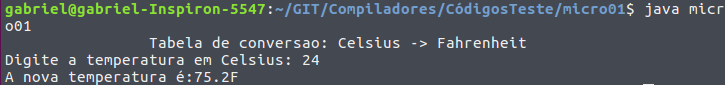
\includegraphics[scale=0.6]{Figures/micro01}
	\end{figure}
	
	\subsubsection{Algoritmo micro02}
	
	\begin{lstlisting}[caption=Código em Java,language=java]
import java.util.Scanner;

public class micro02
{
	public static void main(String[] args)
	{
		Scanner s = new Scanner(System.in);
		int num1 , num2 ;
		System.out.print("Digite o primeiro numero: ");
		num1 = s.nextInt();
		System.out.print("Digite o segundo numero: ");
		num2 = s.nextInt();
		if(num1 >num2)
			System.out.print("O primeiro numero "+num1+" e maior que o segundo "+num2);
		else
			System.out.print("O segundo numero "+num2+" e maior que o primeiro "+num1);
	
	}
}	
	
	\end{lstlisting}
	
	\begin{lstlisting}[caption=Código em python,language=Python]
def micro02():
	num1, num2 = 0 , 0
	print("Digite o primeiro numero: ")
	num1 = int(input())
	print("Digite o segundo numero: ")
	num2 = int(input())
	
	if num1 > num2:
		print("O primeiro numero "+str(num1)+" e maior que o segundo "+str(num2),end="")
	else:
		print("O segundo numero "+str(num2)+" e maior que o primeiro "+str(num1),end="")
	
	
	\end{lstlisting}
	
	\begin{lstlisting}[caption=Smali resultante do .java,language=java]
.class public Lmicro02;
.super Ljava/lang/Object;
.source "micro02.java"


# direct methods
.method public constructor <init>()V
	.registers 3
	
	.prologue
	.line 3
	move-object v0, p0
	
	move-object v1, v0
	
	invoke-direct {v1}, Ljava/lang/Object;-><init>()V
	
	return-void
.end method

.method public static main([Ljava/lang/String;)V
	.registers 9
	
	.prologue
	.line 7
	move-object v0, p0
	
	new-instance v4, Ljava/util/Scanner;
	
	move-object v7, v4
	
	move-object v4, v7
	
	move-object v5, v7
	
	sget-object v6, Ljava/lang/System;->in:Ljava/io/InputStream;
	
	invoke-direct {v5, v6}, Ljava/util/Scanner;-><init>(Ljava/io/InputStream;)V
	
	move-object v1, v4
	
	.line 9
	sget-object v4, Ljava/lang/System;->out:Ljava/io/PrintStream;
	
	const-string v5, "Digite o primeiro numero: "
	
	invoke-virtual {v4, v5}, Ljava/io/PrintStream;->print(Ljava/lang/String;)V
	
	.line 10
	move-object v4, v1
	
	invoke-virtual {v4}, Ljava/util/Scanner;->nextInt()I
	
	move-result v4
	
	move v2, v4
	
	.line 11
	sget-object v4, Ljava/lang/System;->out:Ljava/io/PrintStream;
	
	const-string v5, "Digite o segundo numero: "
	
	invoke-virtual {v4, v5}, Ljava/io/PrintStream;->print(Ljava/lang/String;)V
	
	.line 12
	move-object v4, v1
	
	invoke-virtual {v4}, Ljava/util/Scanner;->nextInt()I
	
	move-result v4
	
	move v3, v4
	
	.line 13
	move v4, v2
	
	move v5, v3
	
	if-le v4, v5, :cond_52
	
	.line 14
	sget-object v4, Ljava/lang/System;->out:Ljava/io/PrintStream;
	
	new-instance v5, Ljava/lang/StringBuffer;
	
	move-object v7, v5
	
	move-object v5, v7
	
	move-object v6, v7
	
	invoke-direct {v6}, Ljava/lang/StringBuffer;-><init>()V
	
	const-string v6, "O primeiro numero "
	
	invoke-virtual {v5, v6}, Ljava/lang/StringBuffer;->append(Ljava/lang/String;)Ljava/lang/StringBuffer;
	
	move-result-object v5
	
	move v6, v2
	
	invoke-virtual {v5, v6}, Ljava/lang/StringBuffer;->append(I)Ljava/lang/StringBuffer;
	
	move-result-object v5
	
	const-string v6, " e maior que o segundo "
	
	invoke-virtual {v5, v6}, Ljava/lang/StringBuffer;->append(Ljava/lang/String;)Ljava/lang/StringBuffer;
	
	move-result-object v5
	
	move v6, v3
	
	invoke-virtual {v5, v6}, Ljava/lang/StringBuffer;->append(I)Ljava/lang/StringBuffer;
	
	move-result-object v5
	
	invoke-virtual {v5}, Ljava/lang/StringBuffer;->toString()Ljava/lang/String;
	
	move-result-object v5
	
	invoke-virtual {v4, v5}, Ljava/io/PrintStream;->print(Ljava/lang/String;)V
	
	.line 18
	:goto_51
	return-void
	
	.line 16
	:cond_52
	sget-object v4, Ljava/lang/System;->out:Ljava/io/PrintStream;
	
	new-instance v5, Ljava/lang/StringBuffer;
	
	move-object v7, v5
	
	move-object v5, v7
	
	move-object v6, v7
	
	invoke-direct {v6}, Ljava/lang/StringBuffer;-><init>()V
	
	const-string v6, "O segundo numero "
	
	invoke-virtual {v5, v6}, Ljava/lang/StringBuffer;->append(Ljava/lang/String;)Ljava/lang/StringBuffer;
	
	move-result-object v5
	
	move v6, v3
	
	invoke-virtual {v5, v6}, Ljava/lang/StringBuffer;->append(I)Ljava/lang/StringBuffer;
	
	move-result-object v5
	
	const-string v6, " e maior que o primeiro "
	
	invoke-virtual {v5, v6}, Ljava/lang/StringBuffer;->append(Ljava/lang/String;)Ljava/lang/StringBuffer;
	
	move-result-object v5
	
	move v6, v2
	
	invoke-virtual {v5, v6}, Ljava/lang/StringBuffer;->append(I)Ljava/lang/StringBuffer;
	
	move-result-object v5
	
	invoke-virtual {v5}, Ljava/lang/StringBuffer;->toString()Ljava/lang/String;
	
	move-result-object v5
	
	invoke-virtual {v4, v5}, Ljava/io/PrintStream;->print(Ljava/lang/String;)V
	
	goto :goto_51
.end method	
	
	\end{lstlisting}
	
	{\large{\textbf{Saída}}}
	
	\begin{figure}[!h]
		\centering
		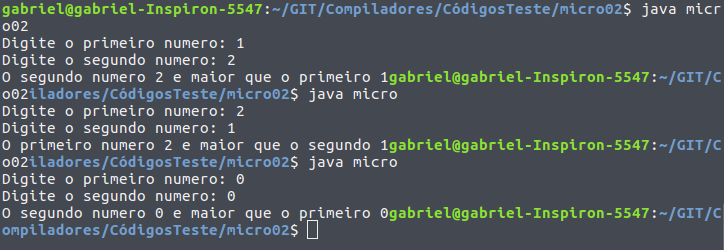
\includegraphics[scale=0.6]{Figures/micro02}
	\end{figure}
	
	\newpage
	\subsubsection{Algoritmo micro03}
	
	\begin{lstlisting}[caption=Código em Java,language=java]
import java.util.Scanner;

public class micro03
{
	public static void main(String[] args)
	{
		Scanner s = new Scanner(System.in);
		int numero;
		System.out.print("Digite um numero: ");
		numero = s.nextInt();
		
		if(numero >= 100)
		{
			if(numero <=200)
				System.out.println("O numero esta no intervalo entre 100 e 200");
			else
				System.out.println("O numero nao esta no intervalo entre 100 e 200");
		}
		else
			System.out.println("O numero nao esta no intervalo entre 100 e 200");
	}
}		
		
	\end{lstlisting}
	
	\begin{lstlisting}[caption=Código em python,language=Python]
def micro03():
	numero =0
	print("Digite um numero: ",end="")
	numero = int(input())
	if numero>= 100:
		if numero<= 200:
			print("O numero esta no intervalo entre 100 e 200")
		else:
			print("O numero nao esta no intervalo entre 100 e 200")
	else:
		print("O numero nao esta no intervalo entre 100 e 200")	
	
	\end{lstlisting}
	
	\begin{lstlisting}[caption=Smali resultante do .java,language=java]
.class public Lmicro03;
.super Ljava/lang/Object;
.source "micro03.java"


# direct methods
.method public constructor <init>()V
	.registers 3
	
	.prologue
	.line 3
	move-object v0, p0
	
	move-object v1, v0
	
	invoke-direct {v1}, Ljava/lang/Object;-><init>()V
	
	return-void
.end method

.method public static main([Ljava/lang/String;)V
	.registers 8
	
	.prologue
	.line 7
	move-object v0, p0
	
	new-instance v3, Ljava/util/Scanner;
	
	move-object v6, v3
	
	move-object v3, v6
	
	move-object v4, v6
	
	sget-object v5, Ljava/lang/System;->in:Ljava/io/InputStream;
	
	invoke-direct {v4, v5}, Ljava/util/Scanner;-><init>(Ljava/io/InputStream;)V
	
	move-object v1, v3
	
	.line 9
	sget-object v3, Ljava/lang/System;->out:Ljava/io/PrintStream;
	
	const-string v4, "Digite um numero: "
	
	invoke-virtual {v3, v4}, Ljava/io/PrintStream;->print(Ljava/lang/String;)V
	
	.line 10
	move-object v3, v1
	
	invoke-virtual {v3}, Ljava/util/Scanner;->nextInt()I
	
	move-result v3
	
	move v2, v3
	
	.line 12
	move v3, v2
	
	const/16 v4, 0x64
	
	if-lt v3, v4, :cond_33
	
	.line 14
	move v3, v2
	
	const/16 v4, 0xc8
	
	if-gt v3, v4, :cond_2b
	
	.line 15
	sget-object v3, Ljava/lang/System;->out:Ljava/io/PrintStream;
	
	const-string v4, "O numero esta no intervalo entre 100 e 200"
	
	invoke-virtual {v3, v4}, Ljava/io/PrintStream;->println(Ljava/lang/String;)V
	
	.line 21
	:goto_2a
	return-void
	
	.line 17
	:cond_2b
	sget-object v3, Ljava/lang/System;->out:Ljava/io/PrintStream;
	
	const-string v4, "O numero nao esta no intervalo entre 100 e 200"
	
	invoke-virtual {v3, v4}, Ljava/io/PrintStream;->println(Ljava/lang/String;)V
	
	goto :goto_2a
	
	.line 20
	:cond_33
	sget-object v3, Ljava/lang/System;->out:Ljava/io/PrintStream;
	
	const-string v4, "O numero nao esta no intervalo entre 100 e 200"
	
	invoke-virtual {v3, v4}, Ljava/io/PrintStream;->println(Ljava/lang/String;)V
	
	goto :goto_2a
.end method	
	
	\end{lstlisting}
	
	O comando \texttt{if-gt}(Greater than) compara dois registradores e se a condição for satisfeita, vai para o target, senão continua normalmente. O \texttt{if-lt}(Less than) funciona de forma análoga. O programa trata o primeiro if na linha 63 que é o caso do numero ser maior que 100. O if seguinte, na linha 70 verifica se \texttt{if-greater than v3 = 100 v4 =200}.
	
	Os números atrbuídos aos registradores sempre estão em formato hexadecimal.\\
	
	{\large{\textbf{Saída}}}
	
	\begin{figure}[!h]
		\centering
		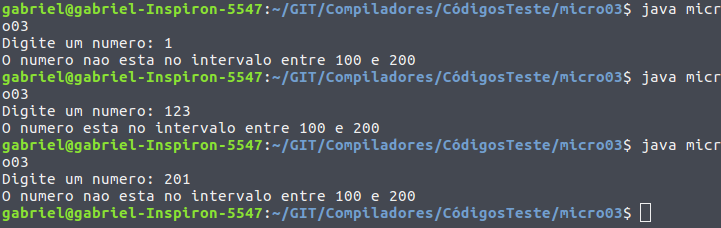
\includegraphics[scale=0.6]{Figures/micro03}
	\end{figure}
	
	\subsubsection{Algoritmo micro04}
	
	\begin{lstlisting}[caption=Código em Java,language=java]
import java.util.Scanner;

public class micro04
{
	public static void main(String[] args)
	{
		Scanner s = new Scanner(System.in);
		int x=0,num=0,intervalo =0;
		
		for (x=0;x<5;x++){
		System.out.print("Digite o numero: ");
		num = s.nextInt();
		if( num >=10)
			if (num <=150)
				intervalo = intervalo +1;
		}
		
		System.out.println("Ao total, foram digitados "+intervalo+" numeros no intervalo entre 10 e 150");
	}
}	
	
	\end{lstlisting}
	
	\begin{lstlisting}[caption=Código em python,language=Python]
def micro04():
	x,num,intervalo = 0,0,0
	
	for x in range(5):
		print("Digite o numero: ",end="")
		num = int(input())
		if num >=10:
			if num <=150:
				intervalo = intervalo +1
	
	print("Ao total, foram digitados "+str(intervalo)+" numeros no intervalo entre 10 e 150")	
	
	\end{lstlisting}
	
	\begin{lstlisting}[caption=Smali resultante do .java,language=java]
.class public Lmicro04;
.super Ljava/lang/Object;
.source "micro04.java"


# direct methods
.method public constructor <init>()V
	.registers 3
	
	.prologue
	.line 3
	move-object v0, p0
	
	move-object v1, v0
	
	invoke-direct {v1}, Ljava/lang/Object;-><init>()V
	
	return-void
.end method

.method public static main([Ljava/lang/String;)V
	.registers 10
	
	.prologue
	.line 7
	move-object v0, p0
	
	new-instance v5, Ljava/util/Scanner;
	
	move-object v8, v5
	
	move-object v5, v8
	
	move-object v6, v8
	
	sget-object v7, Ljava/lang/System;->in:Ljava/io/InputStream;
	
	invoke-direct {v6, v7}, Ljava/util/Scanner;-><init>(Ljava/io/InputStream;)V
	
	move-object v1, v5
	
	.line 8
	const/4 v5, 0x0
	
	move v2, v5
	
	const/4 v5, 0x0
	
	move v3, v5
	
	const/4 v5, 0x0
	
	move v4, v5
	
	.line 10
	const/4 v5, 0x0
	
	move v2, v5
	
	:goto_14
	move v5, v2
	
	const/4 v6, 0x5
	
	if-ge v5, v6, :cond_37
	
	.line 11
	sget-object v5, Ljava/lang/System;->out:Ljava/io/PrintStream;
	
	const-string v6, "Digite o numero: "
	
	invoke-virtual {v5, v6}, Ljava/io/PrintStream;->print(Ljava/lang/String;)V
	
	.line 12
	move-object v5, v1
	
	invoke-virtual {v5}, Ljava/util/Scanner;->nextInt()I
	
	move-result v5
	
	move v3, v5
	
	.line 13
	move v5, v3
	
	const/16 v6, 0xa
	
	if-lt v5, v6, :cond_34
	
	.line 14
	move v5, v3
	
	const/16 v6, 0x96
	
	if-gt v5, v6, :cond_34
	
	.line 15
	move v5, v4
	
	const/4 v6, 0x1
	
	add-int/lit8 v5, v5, 0x1
	
	move v4, v5
	
	.line 10
	:cond_34
	add-int/lit8 v2, v2, 0x1
	
	goto :goto_14
	
	.line 18
	:cond_37
	sget-object v5, Ljava/lang/System;->out:Ljava/io/PrintStream;
	
	new-instance v6, Ljava/lang/StringBuffer;
	
	move-object v8, v6
	
	move-object v6, v8
	
	move-object v7, v8
	
	invoke-direct {v7}, Ljava/lang/StringBuffer;-><init>()V
	
	const-string v7, "Ao total, foram digitados "
	
	invoke-virtual {v6, v7}, Ljava/lang/StringBuffer;->append(Ljava/lang/String;)Ljava/lang/StringBuffer;
	
	move-result-object v6
	
	move v7, v4
	
	invoke-virtual {v6, v7}, Ljava/lang/StringBuffer;->append(I)Ljava/lang/StringBuffer;
	
	move-result-object v6
	
	const-string v7, " numeros no intervalo entre 10 e 150"
	
	invoke-virtual {v6, v7}, Ljava/lang/StringBuffer;->append(Ljava/lang/String;)Ljava/lang/StringBuffer;
	
	move-result-object v6
	
	invoke-virtual {v6}, Ljava/lang/StringBuffer;->toString()Ljava/lang/String;
	
	move-result-object v6
	
	invoke-virtual {v5, v6}, Ljava/io/PrintStream;->println(Ljava/lang/String;)V
	
	.line 19
	return-void
.end method	
	
	\end{lstlisting}
	
	Esse .smali é parecido com o anterior. A diferença principal é o uso do for que, nesse código em .smali é representado por if juntamente com o target.
	
	{\large{\textbf{Saída}}}
	
	\begin{figure}[!h]
		\centering
		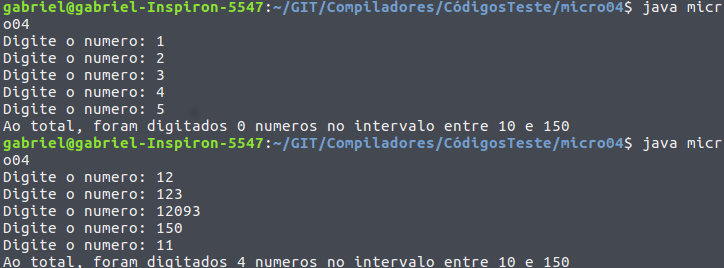
\includegraphics[scale=0.6]{Figures/micro04}
	\end{figure}	
	
	
	\subsubsection{Algoritmo micro05}
	
	Algoritmos com switch são incompatíveis com o java -source 1.4. Por isso, foi usado o 1.7. Além disso, o Python não possui switch-case, então foi feito uma versão equivalente usando if e else.
	
	\begin{lstlisting}[caption=Código em Java,language=java]
import java.util.Scanner;

public class micro05
{
	public static void main(String[] args)
	{
		Scanner s = new Scanner(System.in);
		int x=0,h=0,m =0;
		String nome, sexo;
		
		for (x=0;x<5;x++){
			System.out.print("Digite o nome: ");
			nome = s.nextLine();
			System.out.print("H - Homem ou M - Mulher");
			sexo = s.nextLine();
			
			switch(sexo){
				case "H":
					h = h +1;
					break;
				case "M":
					m = m +1;
					break;
				default:
					System.out.println("Sexo so pode ser H ou M!");
			}	
		}
	
		System.out.println("Foram inseridos "+h+" Homens");
		System.out.println("Foram inseridas "+m+" Mulheres");
	}
}	
	
	\end{lstlisting}
	
	\begin{lstlisting}[caption=Código em python,language=Python]
def micro05():
	x,h,h = 0,0,0
	nome,sexo = "",""
	
	for x in range(5):
		print("Digite o nome: ",end="")
		nome = input()
		print("H - Homem ou M - Mulher",end="")
		sexo = input()
		if sexo == "H":
			h = h+1
		elif sexo == "M":
			m = m+1
		else:
			print("Sexo so pode ser H ou M!")
	
	print("Foram inseridos "+h+" Homens")
	print("Foram inseridas "+m+" Mulheres")	
	
	\end{lstlisting}
	
	\begin{lstlisting}[caption=Smali resultante do .java,language=java]
.class public Lmicro05;
.super Ljava/lang/Object;
.source "micro05.java"


# direct methods
.method public constructor <init>()V
	.registers 3
	
	.prologue
	.line 3
	move-object v0, p0
	
	move-object v1, v0
	
	invoke-direct {v1}, Ljava/lang/Object;-><init>()V
	
	return-void
.end method

.method public static main([Ljava/lang/String;)V
	.registers 14
	
	.prologue
	.line 7
	move-object v0, p0
	
	new-instance v9, Ljava/util/Scanner;
	
	move-object v12, v9
	
	move-object v9, v12
	
	move-object v10, v12
	
	sget-object v11, Ljava/lang/System;->in:Ljava/io/InputStream;
	
	invoke-direct {v10, v11}, Ljava/util/Scanner;-><init>(Ljava/io/InputStream;)V
	
	move-object v1, v9
	
	.line 8
	const/4 v9, 0x0
	
	move v2, v9
	
	const/4 v9, 0x0
	
	move v3, v9
	
	const/4 v9, 0x0
	
	move v4, v9
	
	.line 11
	const/4 v9, 0x0
	
	move v2, v9
	
	:goto_14
	move v9, v2
	
	const/4 v10, 0x5
	
	if-ge v9, v10, :cond_70
	
	.line 12
	sget-object v9, Ljava/lang/System;->out:Ljava/io/PrintStream;
	
	const-string v10, "Digite o nome: "
	
	invoke-virtual {v9, v10}, Ljava/io/PrintStream;->print(Ljava/lang/String;)V
	
	.line 13
	move-object v9, v1
	
	invoke-virtual {v9}, Ljava/util/Scanner;->nextLine()Ljava/lang/String;
	
	move-result-object v9
	
	move-object v5, v9
	
	.line 14
	sget-object v9, Ljava/lang/System;->out:Ljava/io/PrintStream;
	
	const-string v10, "H - Homem ou M - Mulher"
	
	invoke-virtual {v9, v10}, Ljava/io/PrintStream;->print(Ljava/lang/String;)V
	
	.line 15
	move-object v9, v1
	
	invoke-virtual {v9}, Ljava/util/Scanner;->nextLine()Ljava/lang/String;
	
	move-result-object v9
	
	move-object v6, v9
	
	.line 17
	move-object v9, v6
	
	move-object v7, v9
	
	const/4 v9, -0x1
	
	move v8, v9
	
	move-object v9, v7
	
	invoke-virtual {v9}, Ljava/lang/String;->hashCode()I
	
	move-result v9
	
	sparse-switch v9, :sswitch_data_b6
	
	:cond_3e
	:goto_3e
	move v9, v8
	
	packed-switch v9, :pswitch_data_c0
	
	.line 25
	sget-object v9, Ljava/lang/System;->out:Ljava/io/PrintStream;
	
	const-string v10, "Sexo so pode ser H ou M!"
	
	invoke-virtual {v9, v10}, Ljava/io/PrintStream;->println(Ljava/lang/String;)V
	
	.line 11
	:goto_49
	add-int/lit8 v2, v2, 0x1
	
	goto :goto_14
	
	.line 17
	:sswitch_4c
	move-object v9, v7
	
	const-string v10, "H"
	
	invoke-virtual {v9, v10}, Ljava/lang/String;->equals(Ljava/lang/Object;)Z
	
	move-result v9
	
	if-eqz v9, :cond_3e
	
	const/4 v9, 0x0
	
	move v8, v9
	
	goto :goto_3e
	
	:sswitch_58
	move-object v9, v7
	
	const-string v10, "M"
	
	invoke-virtual {v9, v10}, Ljava/lang/String;->equals(Ljava/lang/Object;)Z
	
	move-result v9
	
	if-eqz v9, :cond_3e
	
	const/4 v9, 0x1
	
	move v8, v9
	
	goto :goto_3e
	
	.line 19
	:pswitch_64
	move v9, v3
	
	const/4 v10, 0x1
	
	add-int/lit8 v9, v9, 0x1
	
	move v3, v9
	
	.line 20
	goto :goto_49
	
	.line 22
	:pswitch_6a
	move v9, v4
	
	const/4 v10, 0x1
	
	add-int/lit8 v9, v9, 0x1
	
	move v4, v9
	
	.line 23
	goto :goto_49
	
	.line 29
	:cond_70
	sget-object v9, Ljava/lang/System;->out:Ljava/io/PrintStream;
	
	new-instance v10, Ljava/lang/StringBuilder;
	
	move-object v12, v10
	
	move-object v10, v12
	
	move-object v11, v12
	
	invoke-direct {v11}, Ljava/lang/StringBuilder;-><init>()V
	
	const-string v11, "Foram inseridos "
	
	invoke-virtual {v10, v11}, Ljava/lang/StringBuilder;->append(Ljava/lang/String;)Ljava/lang/StringBuilder;
	
	move-result-object v10
	
	move v11, v3
	
	invoke-virtual {v10, v11}, Ljava/lang/StringBuilder;->append(I)Ljava/lang/StringBuilder;
	
	move-result-object v10
	
	const-string v11, " Homens"
	
	invoke-virtual {v10, v11}, Ljava/lang/StringBuilder;->append(Ljava/lang/String;)Ljava/lang/StringBuilder;
	
	move-result-object v10
	
	invoke-virtual {v10}, Ljava/lang/StringBuilder;->toString()Ljava/lang/String;
	
	move-result-object v10
	
	invoke-virtual {v9, v10}, Ljava/io/PrintStream;->println(Ljava/lang/String;)V
	
	.line 30
	sget-object v9, Ljava/lang/System;->out:Ljava/io/PrintStream;
	
	new-instance v10, Ljava/lang/StringBuilder;
	
	move-object v12, v10
	
	move-object v10, v12
	
	move-object v11, v12
	
	invoke-direct {v11}, Ljava/lang/StringBuilder;-><init>()V
	
	const-string v11, "Foram inseridas "
	
	invoke-virtual {v10, v11}, Ljava/lang/StringBuilder;->append(Ljava/lang/String;)Ljava/lang/StringBuilder;
	
	move-result-object v10
	
	move v11, v4
	
	invoke-virtual {v10, v11}, Ljava/lang/StringBuilder;->append(I)Ljava/lang/StringBuilder;
	
	move-result-object v10
	
	const-string v11, " Mulheres"
	
	invoke-virtual {v10, v11}, Ljava/lang/StringBuilder;->append(Ljava/lang/String;)Ljava/lang/StringBuilder;
	
	move-result-object v10
	
	invoke-virtual {v10}, Ljava/lang/StringBuilder;->toString()Ljava/lang/String;
	
	move-result-object v10
	
	invoke-virtual {v9, v10}, Ljava/io/PrintStream;->println(Ljava/lang/String;)V
	
	.line 31
	return-void
	
	.line 17
	nop
	
	:sswitch_data_b6
	.sparse-switch
	0x48 -> :sswitch_4c
	0x4d -> :sswitch_58
	.end sparse-switch
	
	:pswitch_data_c0
	.packed-switch 0x0
	:pswitch_64
	:pswitch_6a
	.end packed-switch
.end method	
	
	\end{lstlisting}
	
	O uso do switch é representado por \texttt{.sparse-switch} \texttt{.packed-switch}\\
	
	\begin{itemize}
		\item \textbf{packed-switch}: o packed switch funciona de forma esquivalente ao sparse.
		
		\item \textbf{sparse-switch}: é montado uma tabela de constantes. Se na tabela não for achado o caso esperado, o código segue para o default.
	\end{itemize}
	
	{\large{\textbf{Saída}}}
	
	\begin{figure}[!h]
		\centering
		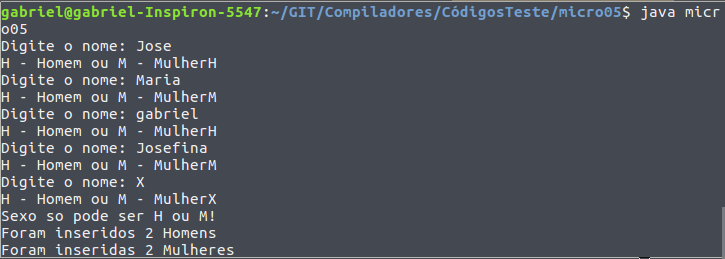
\includegraphics[scale=0.6]{Figures/micro05}
	\end{figure}
	
	\subsubsection{Algoritmo micro06}
	
	\begin{lstlisting}[caption=Código em Java,language=java]
import java.util.Scanner;

public class micro06
{
	public static void main(String[] args)
	{
		Scanner s = new Scanner(System.in);
		int numero=0;
		System.out.print("Digite um numero de 1 a 5: ");
		numero = s.nextInt();
		switch(numero)
		{
		case 1:
			System.out.println("Um");
			break;
		case 2:
			System.out.println("Dois");
			break;
		case 3:
			System.out.println("Tres");
			break;
		case 4:
			System.out.println("Quatro");
			break;
		case 5:
			System.out.println("Cinco");
			break;
		default:
			System.out.println("Numero Invalido");
		}
	
	}
}	
	
	\end{lstlisting}
	
	\begin{lstlisting}[caption=Código em python,language=Python]
def micro06():
	numero = 0
	
	print("Digite um numero de 1 a 5: ",end="")
	numero = int(input())
	if numero ==1: 
		print("Um")
	elif numero == 2:
		print("Dois")
	elif numero ==3:
		print("Tres")
	elif numero ==4:
		print("Quatro")
	elif numero ==5:
		print("Cinco")
	else:
		print("Numero Invalido!!!")
	
	
	\end{lstlisting}
	
	\begin{lstlisting}[caption=Smali resultante do .java,language=java]
.class public Lmicro06;
.super Ljava/lang/Object;
.source "micro06.java"


# direct methods
.method public constructor <init>()V
	.registers 3
	
	.prologue
	.line 3
	move-object v0, p0
	
	move-object v1, v0
	
	invoke-direct {v1}, Ljava/lang/Object;-><init>()V
	
	return-void
.end method

.method public static main([Ljava/lang/String;)V
	.registers 8
	
	.prologue
	.line 7
	move-object v0, p0
	
	new-instance v3, Ljava/util/Scanner;
	
	move-object v6, v3
	
	move-object v3, v6
	
	move-object v4, v6
	
	sget-object v5, Ljava/lang/System;->in:Ljava/io/InputStream;
	
	invoke-direct {v4, v5}, Ljava/util/Scanner;-><init>(Ljava/io/InputStream;)V
	
	move-object v1, v3
	
	.line 8
	const/4 v3, 0x0
	
	move v2, v3
	
	.line 9
	sget-object v3, Ljava/lang/System;->out:Ljava/io/PrintStream;
	
	const-string v4, "Digite um numero de 1 a 5: "
	
	invoke-virtual {v3, v4}, Ljava/io/PrintStream;->print(Ljava/lang/String;)V
	
	.line 10
	move-object v3, v1
	
	invoke-virtual {v3}, Ljava/util/Scanner;->nextInt()I
	
	move-result v3
	
	move v2, v3
	
	.line 11
	move v3, v2
	
	packed-switch v3, :pswitch_data_50
	
	.line 29
	sget-object v3, Ljava/lang/System;->out:Ljava/io/PrintStream;
	
	const-string v4, "Numero Invalido"
	
	invoke-virtual {v3, v4}, Ljava/io/PrintStream;->println(Ljava/lang/String;)V
	
	.line 32
	:goto_26
	return-void
	
	.line 14
	:pswitch_27
	sget-object v3, Ljava/lang/System;->out:Ljava/io/PrintStream;
	
	const-string v4, "Um"
	
	invoke-virtual {v3, v4}, Ljava/io/PrintStream;->println(Ljava/lang/String;)V
	
	.line 15
	goto :goto_26
	
	.line 17
	:pswitch_2f
	sget-object v3, Ljava/lang/System;->out:Ljava/io/PrintStream;
	
	const-string v4, "Dois"
	
	invoke-virtual {v3, v4}, Ljava/io/PrintStream;->println(Ljava/lang/String;)V
	
	.line 18
	goto :goto_26
	
	.line 20
	:pswitch_37
	sget-object v3, Ljava/lang/System;->out:Ljava/io/PrintStream;
	
	const-string v4, "Tres"
	
	invoke-virtual {v3, v4}, Ljava/io/PrintStream;->println(Ljava/lang/String;)V
	
	.line 21
	goto :goto_26
	
	.line 23
	:pswitch_3f
	sget-object v3, Ljava/lang/System;->out:Ljava/io/PrintStream;
	
	const-string v4, "Quatro"
	
	invoke-virtual {v3, v4}, Ljava/io/PrintStream;->println(Ljava/lang/String;)V
	
	.line 24
	goto :goto_26
	
	.line 26
	:pswitch_47
	sget-object v3, Ljava/lang/System;->out:Ljava/io/PrintStream;
	
	const-string v4, "Cinco"
	
	invoke-virtual {v3, v4}, Ljava/io/PrintStream;->println(Ljava/lang/String;)V
	
	.line 27
	goto :goto_26
	
	.line 11
	nop
	
	:pswitch_data_50
	.packed-switch 0x1
	:pswitch_27
	:pswitch_2f
	:pswitch_37
	:pswitch_3f
	:pswitch_47
	.end packed-switch
.end method	
	
	\end{lstlisting}
	
	{\large{\textbf{Saída}}}
	
	\begin{figure}[!h]
		\centering
		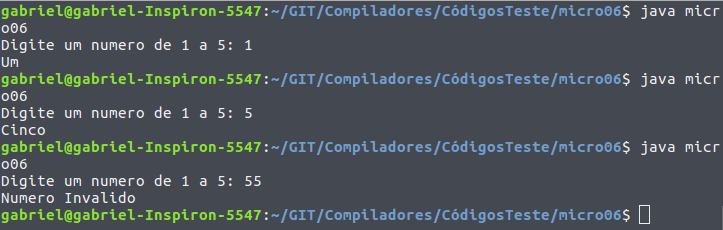
\includegraphics[scale=0.6]{Figures/micro06}
	\end{figure}
	
	\subsubsection{Algoritmo micro07}
	
	\begin{lstlisting}[caption=Código em Java,language=java]
import java.util.Scanner;

public class micro07
{
public static void main(String[] args)
	{
		Scanner s = new Scanner(System.in);
		int numero=0, programa=1;
		char opc;
		while( programa ==1){
			System.out.print("Digite um numero: ");
			numero = s.nextInt();
			
			if (numero>0)
				System.out.println("Positivo");
			else
			{
				if (numero==0)
					System.out.println("O numero e igual a 0");
				if (numero <0)
					System.out.println("Negativo");
			}
			System.out.print("Deseja Finalizar? (S/N) ");
			opc = s.next().charAt(0);
			if (opc == 'S')
				programa = 0;
		}
	}
}	
	
	\end{lstlisting}
	
	\begin{lstlisting}[caption=Código em python,language=Python]
def micro07():
	numero ,programa= 0,1
	opc = ""
	
	while programa ==1:
		print("Digite um numero: ",end="")
		numero = int(input())
		
		if numero>0:
			print("Positivo")
		else:
			if numero==0:
				print("O numero e igual a 0")
			if numero <0:
				print("Negativo")
			
		print("Deseja Finalizar? (S/N) ",end="")
		opc = input()
		if opc == "S":
			programa = 0	
	
	\end{lstlisting}
	
	\begin{lstlisting}[caption=Smali resultante do .java,language=java]
.class public Lmicro07;
.super Ljava/lang/Object;
.source "micro07.java"


# direct methods
.method public constructor <init>()V
	.registers 3
	
	.prologue
	.line 3
	move-object v0, p0
	
	move-object v1, v0
	
	invoke-direct {v1}, Ljava/lang/Object;-><init>()V
	
	return-void
.end method

.method public static main([Ljava/lang/String;)V
	.registers 10
	
	.prologue
	.line 7
	move-object v0, p0
	
	new-instance v5, Ljava/util/Scanner;
	
	move-object v8, v5
	
	move-object v5, v8
	
	move-object v6, v8
	
	sget-object v7, Ljava/lang/System;->in:Ljava/io/InputStream;
	
	invoke-direct {v6, v7}, Ljava/util/Scanner;-><init>(Ljava/io/InputStream;)V
	
	move-object v1, v5
	
	.line 8
	const/4 v5, 0x0
	
	move v2, v5
	
	const/4 v5, 0x1
	
	move v3, v5
	
	.line 10
	:cond_10
	:goto_10
	move v5, v3
	
	const/4 v6, 0x1
	
	if-ne v5, v6, :cond_5a
	
	.line 11
	sget-object v5, Ljava/lang/System;->out:Ljava/io/PrintStream;
	
	const-string v6, "Digite um n\u00famero: "
	
	invoke-virtual {v5, v6}, Ljava/io/PrintStream;->print(Ljava/lang/String;)V
	
	.line 12
	move-object v5, v1
	
	invoke-virtual {v5}, Ljava/util/Scanner;->nextInt()I
	
	move-result v5
	
	move v2, v5
	
	.line 14
	move v5, v2
	
	if-lez v5, :cond_45
	
	.line 15
	sget-object v5, Ljava/lang/System;->out:Ljava/io/PrintStream;
	
	const-string v6, "Positivo"
	
	invoke-virtual {v5, v6}, Ljava/io/PrintStream;->println(Ljava/lang/String;)V
	
	.line 23
	:cond_2b
	:goto_2b
	sget-object v5, Ljava/lang/System;->out:Ljava/io/PrintStream;
	
	const-string v6, "Deseja Finalizar? (S/N) "
	
	invoke-virtual {v5, v6}, Ljava/io/PrintStream;->print(Ljava/lang/String;)V
	
	.line 24
	move-object v5, v1
	
	invoke-virtual {v5}, Ljava/util/Scanner;->next()Ljava/lang/String;
	
	move-result-object v5
	
	const/4 v6, 0x0
	
	invoke-virtual {v5, v6}, Ljava/lang/String;->charAt(I)C
	
	move-result v5
	
	move v4, v5
	
	.line 25
	move v5, v4
	
	const/16 v6, 0x53
	
	if-ne v5, v6, :cond_10
	
	.line 26
	const/4 v5, 0x0
	
	move v3, v5
	
	goto :goto_10
	
	.line 18
	:cond_45
	move v5, v2
	
	if-nez v5, :cond_4f
	
	.line 19
	sget-object v5, Ljava/lang/System;->out:Ljava/io/PrintStream;
	
	const-string v6, "O numero e igual a 0"
	
	invoke-virtual {v5, v6}, Ljava/io/PrintStream;->println(Ljava/lang/String;)V
	
	.line 20
	:cond_4f
	move v5, v2
	
	if-gez v5, :cond_2b
	
	.line 21
	sget-object v5, Ljava/lang/System;->out:Ljava/io/PrintStream;
	
	const-string v6, "Negativo"
	
	invoke-virtual {v5, v6}, Ljava/io/PrintStream;->println(Ljava/lang/String;)V
	
	goto :goto_2b
	
	.line 28
	:cond_5a
	return-void
.end method	
	
	\end{lstlisting}
	
	Pode-se observar que a linha 58 corresponde ao while uma vez que se não for satisfeita a condição o programa vai para o final.
	
	{\large{\textbf{Saída}}}
	
	\begin{figure}[!h]
		\centering
		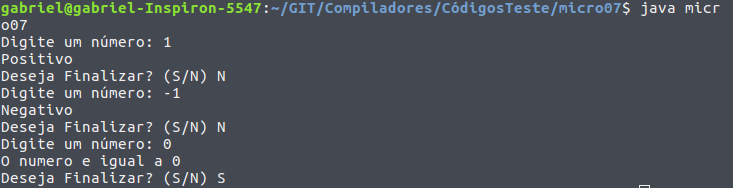
\includegraphics[scale=0.6]{Figures/micro07}
	\end{figure}
	
	\subsubsection{Algoritmo micro08}
	
	\begin{lstlisting}[caption=Código em Java,language=java]
import java.util.Scanner;

public class micro08
	{
	public static void main(String[] args)
		{
			Scanner s = new Scanner(System.in);
			int numero =1;
			while (numero < 0 || numero >0){
				System.out.print("Digite o numero");
				numero = s.nextInt();
				if (numero > 10)
					System.out.println("O numero "+numero+" e maior que 10");
				else
					System.out.println("O numero "+numero+" e menor que 10");
		}
	}
}	
	
	\end{lstlisting}
	
	\begin{lstlisting}[caption=Código em python,language=Python]
def micro08():
	numero =1
	while numero < 0 or numero >0:
		print("Digite o numero",end="")
		numero = int(input())
		if numero > 10:
			print("O numero "+str(numero)+" e maior que 10")
		else:
			print("O numero "+str(numero)+" e menor que 10")
	
	
	\end{lstlisting}
	
	\begin{lstlisting}[caption=Smali resultante do .java,language=java]
.class public Lmicro08;
.super Ljava/lang/Object;
.source "micro08.java"


# direct methods
.method public constructor <init>()V
	.registers 3
	
	.prologue
	.line 3
	move-object v0, p0
	
	move-object v1, v0
	
	invoke-direct {v1}, Ljava/lang/Object;-><init>()V
	
	return-void
.end method

.method public static main([Ljava/lang/String;)V
	.registers 8
	
	.prologue
	.line 7
	move-object v0, p0
	
	new-instance v3, Ljava/util/Scanner;
	
	move-object v6, v3
	
	move-object v3, v6
	
	move-object v4, v6
	
	sget-object v5, Ljava/lang/System;->in:Ljava/io/InputStream;
	
	invoke-direct {v4, v5}, Ljava/util/Scanner;-><init>(Ljava/io/InputStream;)V
	
	move-object v1, v3
	
	.line 8
	const/4 v3, 0x1
	
	move v2, v3
	
	.line 9
	:goto_e
	move v3, v2
	
	if-ltz v3, :cond_14
	
	move v3, v2
	
	if-lez v3, :cond_6c
	
	.line 10
	:cond_14
	sget-object v3, Ljava/lang/System;->out:Ljava/io/PrintStream;
	
	const-string v4, "Digite o numero"
	
	invoke-virtual {v3, v4}, Ljava/io/PrintStream;->print(Ljava/lang/String;)V
	
	.line 11
	move-object v3, v1
	
	invoke-virtual {v3}, Ljava/util/Scanner;->nextInt()I
	
	move-result v3
	
	move v2, v3
	
	.line 12
	move v3, v2
	
	const/16 v4, 0xa
	
	if-le v3, v4, :cond_49
	
	.line 13
	sget-object v3, Ljava/lang/System;->out:Ljava/io/PrintStream;
	
	new-instance v4, Ljava/lang/StringBuffer;
	
	move-object v6, v4
	
	move-object v4, v6
	
	move-object v5, v6
	
	invoke-direct {v5}, Ljava/lang/StringBuffer;-><init>()V
	
	const-string v5, "O numero "
	
	invoke-virtual {v4, v5}, Ljava/lang/StringBuffer;->append(Ljava/lang/String;)Ljava/lang/StringBuffer;
	
	move-result-object v4
	
	move v5, v2
	
	invoke-virtual {v4, v5}, Ljava/lang/StringBuffer;->append(I)Ljava/lang/StringBuffer;
	
	move-result-object v4
	
	const-string v5, " e maior que 10"
	
	invoke-virtual {v4, v5}, Ljava/lang/StringBuffer;->append(Ljava/lang/String;)Ljava/lang/StringBuffer;
	
	move-result-object v4
	
	invoke-virtual {v4}, Ljava/lang/StringBuffer;->toString()Ljava/lang/String;
	
	move-result-object v4
	
	invoke-virtual {v3, v4}, Ljava/io/PrintStream;->println(Ljava/lang/String;)V
	
	goto :goto_e
	
	.line 15
	:cond_49
	sget-object v3, Ljava/lang/System;->out:Ljava/io/PrintStream;
	
	new-instance v4, Ljava/lang/StringBuffer;
	
	move-object v6, v4
	
	move-object v4, v6
	
	move-object v5, v6
	
	invoke-direct {v5}, Ljava/lang/StringBuffer;-><init>()V
	
	const-string v5, "O numero "
	
	invoke-virtual {v4, v5}, Ljava/lang/StringBuffer;->append(Ljava/lang/String;)Ljava/lang/StringBuffer;
	
	move-result-object v4
	
	move v5, v2
	
	invoke-virtual {v4, v5}, Ljava/lang/StringBuffer;->append(I)Ljava/lang/StringBuffer;
	
	move-result-object v4
	
	const-string v5, " e menor que 10"
	
	invoke-virtual {v4, v5}, Ljava/lang/StringBuffer;->append(Ljava/lang/String;)Ljava/lang/StringBuffer;
	
	move-result-object v4
	
	invoke-virtual {v4}, Ljava/lang/StringBuffer;->toString()Ljava/lang/String;
	
	move-result-object v4
	
	invoke-virtual {v3, v4}, Ljava/io/PrintStream;->println(Ljava/lang/String;)V
	
	goto :goto_e
	
	.line 17
	:cond_6c
	return-void
.end method	
	
	\end{lstlisting}
	
	{\large{\textbf{Saída}}}
	
	\begin{figure}[!h]
		\centering
		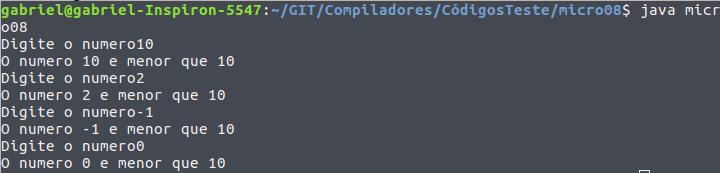
\includegraphics[scale=0.6]{Figures/micro08}
	\end{figure}
	
	
	\subsubsection{Algoritmo micro09}
	
	\begin{lstlisting}[caption=Código em Java,language=java]
import java.util.Scanner;

public class micro09
{
	public static void main(String[] args)
	{
		Scanner s = new Scanner(System.in);
		double preco, venda, novopreco=0 ;
		
		System.out.print("Digite o preco: ");
		preco = s.nextDouble();
		System.out.print("Digite a venda: ");
		venda = s.nextDouble();
		
		if (venda < 500.0 || preco <30.0){
			novopreco = preco + 10.0/100.0 *preco;
		}
		else if ((venda >= 500.0 && venda <1200.0) || (preco >= 30.0 && preco <80.0)){
			novopreco = preco + 15.0/100.0 * preco;
		}
		else if (venda >=1200.0 || preco >=80.0){
			novopreco = preco - 20.0/100.0 * preco;
		}
		
		
		System.out.println("O novo preco e: "+novopreco);
	}
}	
	
	\end{lstlisting}
	
	\begin{lstlisting}[caption=Código em python,language=Python]
def micro09():
	preco, venda, novopreco = 0.0,0.0,0.0
	
	print("Digite o preco: ",end="")
	preco = int(input())
	print("Digite a venda: ",end="")
	venda = int(input())
	if venda < 500 or preco <30:
		novopreco = preco + 10/100 *preco
	elif (venda >= 500 and venda <1200) or (preco >= 30 and preco <80):
		novopreco = preco + 15/100 * preco
	elif venda >=1200 or preco >=80:
		novopreco = preco - 20/100 * preco
	
	print("O novo preco e: "+str(novopreco))
	
	
	\end{lstlisting}
	
	\begin{lstlisting}[caption=Smali resultante do .java,language=java]
.class public Lmicro09;
.super Ljava/lang/Object;
.source "micro09.java"


# direct methods
.method public constructor <init>()V
	.registers 3
	
	.prologue
	.line 3
	move-object v0, p0
	
	move-object v1, v0
	
	invoke-direct {v1}, Ljava/lang/Object;-><init>()V
	
	return-void
.end method

.method public static main([Ljava/lang/String;)V
	.registers 16
	
	.prologue
	.line 7
	move-object v0, p0
	
	new-instance v8, Ljava/util/Scanner;
	
	move-object v14, v8
	
	move-object v8, v14
	
	move-object v9, v14
	
	sget-object v10, Ljava/lang/System;->in:Ljava/io/InputStream;
	
	invoke-direct {v9, v10}, Ljava/util/Scanner;-><init>(Ljava/io/InputStream;)V
	
	move-object v1, v8
	
	.line 8
	const-wide/16 v8, 0x0
	
	move-wide v6, v8
	
	.line 10
	sget-object v8, Ljava/lang/System;->out:Ljava/io/PrintStream;
	
	const-string v9, "Digite o preco: "
	
	invoke-virtual {v8, v9}, Ljava/io/PrintStream;->print(Ljava/lang/String;)V
	
	.line 11
	move-object v8, v1
	
	invoke-virtual {v8}, Ljava/util/Scanner;->nextDouble()D
	
	move-result-wide v8
	
	move-wide v2, v8
	
	.line 12
	sget-object v8, Ljava/lang/System;->out:Ljava/io/PrintStream;
	
	const-string v9, "Digite a venda: "
	
	invoke-virtual {v8, v9}, Ljava/io/PrintStream;->print(Ljava/lang/String;)V
	
	.line 13
	move-object v8, v1
	
	invoke-virtual {v8}, Ljava/util/Scanner;->nextDouble()D
	
	move-result-wide v8
	
	move-wide v4, v8
	
	.line 15
	move-wide v8, v4
	
	const-wide v10, 0x407f400000000000L    # 500.0
	
	cmpg-double v8, v8, v10
	
	if-ltz v8, :cond_3a
	
	move-wide v8, v2
	
	const-wide/high16 v10, 0x403e000000000000L    # 30.0
	
	cmpg-double v8, v8, v10
	
	if-gez v8, :cond_61
	
	.line 16
	:cond_3a
	move-wide v8, v2
	
	const-wide v10, 0x3fb999999999999aL    # 0.1
	
	move-wide v12, v2
	
	mul-double/2addr v10, v12
	
	add-double/2addr v8, v10
	
	move-wide v6, v8
	
	.line 26
	:cond_44
	:goto_44
	sget-object v8, Ljava/lang/System;->out:Ljava/io/PrintStream;
	
	new-instance v9, Ljava/lang/StringBuffer;
	
	move-object v14, v9
	
	move-object v9, v14
	
	move-object v10, v14
	
	invoke-direct {v10}, Ljava/lang/StringBuffer;-><init>()V
	
	const-string v10, "O novo preco e: "
	
	invoke-virtual {v9, v10}, Ljava/lang/StringBuffer;->append(Ljava/lang/String;)Ljava/lang/StringBuffer;
	
	move-result-object v9
	
	move-wide v10, v6
	
	invoke-virtual {v9, v10, v11}, Ljava/lang/StringBuffer;->append(D)Ljava/lang/StringBuffer;
	
	move-result-object v9
	
	invoke-virtual {v9}, Ljava/lang/StringBuffer;->toString()Ljava/lang/String;
	
	move-result-object v9
	
	invoke-virtual {v8, v9}, Ljava/io/PrintStream;->println(Ljava/lang/String;)V
	
	.line 27
	return-void
	
	.line 18
	:cond_61
	move-wide v8, v4
	
	const-wide v10, 0x407f400000000000L    # 500.0
	
	cmpl-double v8, v8, v10
	
	if-ltz v8, :cond_75
	
	move-wide v8, v4
	
	const-wide v10, 0x4092c00000000000L    # 1200.0
	
	cmpg-double v8, v8, v10
	
	if-ltz v8, :cond_83
	
	:cond_75
	move-wide v8, v2
	
	const-wide/high16 v10, 0x403e000000000000L    # 30.0
	
	cmpl-double v8, v8, v10
	
	if-ltz v8, :cond_8e
	
	move-wide v8, v2
	
	const-wide/high16 v10, 0x4054000000000000L    # 80.0
	
	cmpg-double v8, v8, v10
	
	if-gez v8, :cond_8e
	
	.line 19
	:cond_83
	move-wide v8, v2
	
	const-wide v10, 0x3fc3333333333333L    # 0.15
	
	move-wide v12, v2
	
	mul-double/2addr v10, v12
	
	add-double/2addr v8, v10
	
	move-wide v6, v8
	
	goto :goto_44
	
	.line 21
	:cond_8e
	move-wide v8, v4
	
	const-wide v10, 0x4092c00000000000L    # 1200.0
	
	cmpl-double v8, v8, v10
	
	if-gez v8, :cond_9f
	
	move-wide v8, v2
	
	const-wide/high16 v10, 0x4054000000000000L    # 80.0
	
	cmpl-double v8, v8, v10
	
	if-ltz v8, :cond_44
	
	.line 22
	:cond_9f
	move-wide v8, v2
	
	const-wide v10, 0x3fc999999999999aL    # 0.2
	
	move-wide v12, v2
	
	mul-double/2addr v10, v12
	
	sub-double/2addr v8, v10
	
	move-wide v6, v8
	
	goto :goto_44
.end method	
	
	\end{lstlisting}
	
	Os \texttt{ifs} que contém duas condições ou mais são desmembrados em dois ou mais ifs. No caso do if que possui a condicional e são usados dois if em smali para fazer um if do java pois o primeiro verifica o lado esquerdo e o segundo o direito. Os dois ifs tem que ser verdadeiros. No caso do ou, apenas um lado da condição é verificado de cada vez e o segundo lado só é verificado se o primeiro falhar.
	
	É interessante observar que quando o número em hexadecimal é muito extenso, o smali comenta automaticamente qual é esse número em decimal(linha 82 e 90)\\
	
	{\large{\textbf{Saída}}}
	
	\begin{figure}[!h]
		\centering
		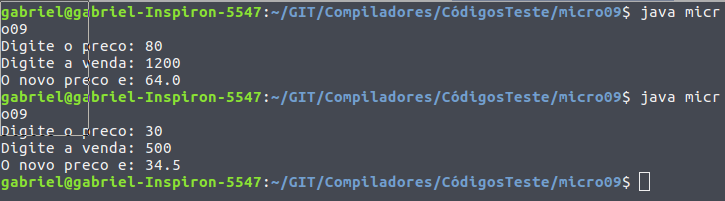
\includegraphics[scale=0.6]{Figures/micro09}
	\end{figure}
	
	\newpage
	
	\subsubsection{Algoritmo micro10}
	
	\begin{lstlisting}[caption=Código em Java,language=java]
import java.util.Scanner;

public class micro10
{
	public static void main(String[] args)
	{
		Scanner s = new Scanner(System.in);
		int numero=0, fat;
		System.out.print("Digite um numero: ");
		numero = s.nextInt();
		fat = fatorial(numero);
		System.out.println("O fatorial de "+numero+" e "+fat);
		
		
	}
		
	public static int fatorial(int n)
	{
		if(n <= 0) return 1;
		else return n* fatorial(n-1);
	}


}	
	
	\end{lstlisting}
	
	\begin{lstlisting}[caption=Código em python,language=Python]
def micro10():
	numero =0
	fat = 0
	print("Digite um numero: ",end="")
	numero = int(input())
	fat = fatorial(numero)
	
	print("O fatorial de "+str(numero)+" e "+str(fat),end="")



def fatorial(n):
	if n <=0:
		return 1
	else:
		return (n * fatorial(n-1))	
	
	\end{lstlisting}
	
	\begin{lstlisting}[caption=Smali resultante do .java,language=java]
.class public Lmicro10;
.super Ljava/lang/Object;
.source "micro10.java"


# direct methods
.method public constructor <init>()V
	.registers 3
	
	.prologue
	.line 3
	move-object v0, p0
	
	move-object v1, v0
	
	invoke-direct {v1}, Ljava/lang/Object;-><init>()V
	
	return-void
.end method

.method public static fatorial(I)I
	.registers 5
	
	.prologue
	.line 18
	move v0, p0
	
	move v1, v0
	
	if-gtz v1, :cond_7
	
	const/4 v1, 0x1
	
	move v0, v1
	
	.line 19
	:goto_6
	return v0
	
	:cond_7
	move v1, v0
	
	move v2, v0
	
	const/4 v3, 0x1
	
	add-int/lit8 v2, v2, -0x1
	
	invoke-static {v2}, Lmicro10;->fatorial(I)I
	
	move-result v2
	
	mul-int/2addr v1, v2
	
	move v0, v1
	
	goto :goto_6
	.end method
	
	.method public static main([Ljava/lang/String;)V
	.registers 9
	
	.prologue
	.line 7
	move-object v0, p0
	
	new-instance v4, Ljava/util/Scanner;
	
	move-object v7, v4
	
	move-object v4, v7
	
	move-object v5, v7
	
	sget-object v6, Ljava/lang/System;->in:Ljava/io/InputStream;
	
	invoke-direct {v5, v6}, Ljava/util/Scanner;-><init>(Ljava/io/InputStream;)V
	
	move-object v1, v4
	
	.line 8
	const/4 v4, 0x0
	
	move v2, v4
	
	.line 9
	sget-object v4, Ljava/lang/System;->out:Ljava/io/PrintStream;
	
	const-string v5, "Digite um numero: "
	
	invoke-virtual {v4, v5}, Ljava/io/PrintStream;->print(Ljava/lang/String;)V
	
	.line 10
	move-object v4, v1
	
	invoke-virtual {v4}, Ljava/util/Scanner;->nextInt()I
	
	move-result v4
	
	move v2, v4
	
	.line 11
	move v4, v2
	
	invoke-static {v4}, Lmicro10;->fatorial(I)I
	
	move-result v4
	
	move v3, v4
	
	.line 12
	sget-object v4, Ljava/lang/System;->out:Ljava/io/PrintStream;
	
	new-instance v5, Ljava/lang/StringBuffer;
	
	move-object v7, v5
	
	move-object v5, v7
	
	move-object v6, v7
	
	invoke-direct {v6}, Ljava/lang/StringBuffer;-><init>()V
	
	const-string v6, "O fatorial de "
	
	invoke-virtual {v5, v6}, Ljava/lang/StringBuffer;->append(Ljava/lang/String;)Ljava/lang/StringBuffer;
	
	move-result-object v5
	
	move v6, v2
	
	invoke-virtual {v5, v6}, Ljava/lang/StringBuffer;->append(I)Ljava/lang/StringBuffer;
	
	move-result-object v5
	
	const-string v6, " e "
	
	invoke-virtual {v5, v6}, Ljava/lang/StringBuffer;->append(Ljava/lang/String;)Ljava/lang/StringBuffer;
	
	move-result-object v5
	
	move v6, v3
	
	invoke-virtual {v5, v6}, Ljava/lang/StringBuffer;->append(I)Ljava/lang/StringBuffer;
	
	move-result-object v5
	
	invoke-virtual {v5}, Ljava/lang/StringBuffer;->toString()Ljava/lang/String;
	
	move-result-object v5
	
	invoke-virtual {v4, v5}, Ljava/io/PrintStream;->println(Ljava/lang/String;)V
	
	.line 15
	return-void
.end method	
	
	\end{lstlisting}
	
	A chamada do fatorial acontece de forma análoga ao java. Pode-se observar isso na linha 49. Na linha 30, é verificado se o parâmetro recebido é maior que 0. Se for maior que 0 o código vai para o target \texttt{:cond\_7} onde outra chamada de fatorial é feita na linha 49 ja mencionada. Caso o número do parâmetro seja 0, o código retorna o parâmetro e começa a resolução da recursão.
	
	{\large{\textbf{Saída}}}
	
	\begin{figure}[!h]
		\centering
		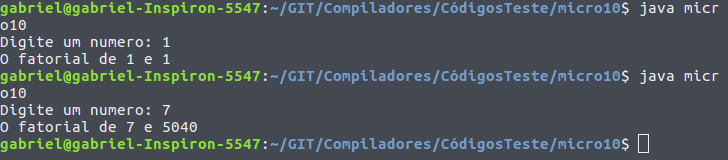
\includegraphics[scale=0.6]{Figures/micro10}
	\end{figure}
	
	\subsubsection{Algoritmo micro11}
	
	\begin{lstlisting}[caption=Código em Java,language=java]
import java.util.Scanner;

public class micro11
{
	public static void main(String[] args)
	{
		Scanner s = new Scanner(System.in);
		int numero=0, x;
		System.out.print("Digite um numero: ");
		numero = s.nextInt();
		x = verifica(numero);
		if(x ==1) System.out.println("Numero Positivo");
		else if (x==0) System.out.println("Zero");
		else System.out.println("Numero Negativo");
	
	}

	public static int verifica(int n){
		int res;
		if(n>0) res =1;
		else if(n<0) res = -1;
		else res = 0;
		
		
		return res;
	}


}	
	
	\end{lstlisting}
	
	\begin{lstlisting}[caption=Código em python,language=Python]
def micro11():
	numero,x =0,0
	print("Digite um numero: ",end="")
	numero = int(input())
	x = verifica(numero)
	if x ==1:
		print("Numero Positivo")
	elif x ==0:
		print("Zero")
	else:
		print("Negativo")

def verifica(n):
	res = 0
	if n>0:
		res = 1
	elif n<0:
		res = -1
	else:
		res = 0
	
	return res	
	
	\end{lstlisting}
	
	\begin{lstlisting}[caption=Smali resultante do .java,language=java]
.class public Lmicro11;
.super Ljava/lang/Object;
.source "micro11.java"


# direct methods
.method public constructor <init>()V
	.registers 3
	
	.prologue
	.line 3
	move-object v0, p0
	
	move-object v1, v0
	
	invoke-direct {v1}, Ljava/lang/Object;-><init>()V
	
	return-void
.end method

.method public static main([Ljava/lang/String;)V
	.registers 9
	
	.prologue
	.line 7
	move-object v0, p0
	
	new-instance v4, Ljava/util/Scanner;
	
	move-object v7, v4
	
	move-object v4, v7
	
	move-object v5, v7
	
	sget-object v6, Ljava/lang/System;->in:Ljava/io/InputStream;
	
	invoke-direct {v5, v6}, Ljava/util/Scanner;-><init>(Ljava/io/InputStream;)V
	
	move-object v1, v4
	
	.line 8
	const/4 v4, 0x0
	
	move v2, v4
	
	.line 9
	sget-object v4, Ljava/lang/System;->out:Ljava/io/PrintStream;
	
	const-string v5, "Digite um numero: "
	
	invoke-virtual {v4, v5}, Ljava/io/PrintStream;->print(Ljava/lang/String;)V
	
	.line 10
	move-object v4, v1
	
	invoke-virtual {v4}, Ljava/util/Scanner;->nextInt()I
	
	move-result v4
	
	move v2, v4
	
	.line 11
	move v4, v2
	
	invoke-static {v4}, Lmicro11;->verifica(I)I
	
	move-result v4
	
	move v3, v4
	
	.line 12
	move v4, v3
	
	const/4 v5, 0x1
	
	if-ne v4, v5, :cond_2d
	
	sget-object v4, Ljava/lang/System;->out:Ljava/io/PrintStream;
	
	const-string v5, "Numero Positivo"
	
	invoke-virtual {v4, v5}, Ljava/io/PrintStream;->println(Ljava/lang/String;)V
	
	.line 16
	:goto_2c
	return-void
	
	.line 13
	:cond_2d
	move v4, v3
	
	if-nez v4, :cond_38
	
	sget-object v4, Ljava/lang/System;->out:Ljava/io/PrintStream;
	
	const-string v5, "Zero"
	
	invoke-virtual {v4, v5}, Ljava/io/PrintStream;->println(Ljava/lang/String;)V
	
	goto :goto_2c
	
	.line 14
	:cond_38
	sget-object v4, Ljava/lang/System;->out:Ljava/io/PrintStream;
	
	const-string v5, "Numero Negativo"
	
	invoke-virtual {v4, v5}, Ljava/io/PrintStream;->println(Ljava/lang/String;)V
	
	goto :goto_2c
	.end method
	
	.method public static verifica(I)I
	.registers 4
	
	.prologue
	.line 20
	move v0, p0
	
	move v2, v0
	
	if-lez v2, :cond_9
	
	const/4 v2, 0x1
	
	move v1, v2
	
	.line 25
	:goto_6
	move v2, v1
	
	move v0, v2
	
	return v0
	
	.line 21
	:cond_9
	move v2, v0
	
	if-gez v2, :cond_f
	
	const/4 v2, -0x1
	
	move v1, v2
	
	goto :goto_6
	
	.line 22
	:cond_f
	const/4 v2, 0x0
	
	move v1, v2
	
	goto :goto_6
.end method	
	
	\end{lstlisting}
	
	{\large{\textbf{Saída}}}
	
	\begin{figure}[!h]
		\centering
		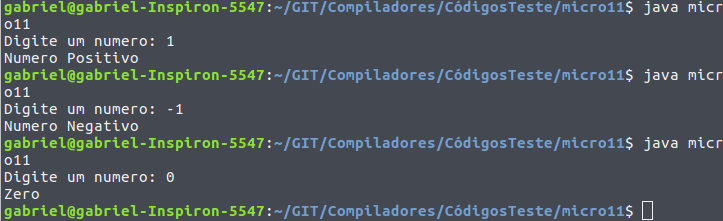
\includegraphics[scale=0.6]{Figures/micro11}
	\end{figure}

\section{Analisador Léxico}

\subsection{Abordagem por Autômato}

	Segue uma versão simplificada (pela facilidade de entender o processo) do autômato, que será implementado em Ocaml, sendo que algumas considerações foram feitas:
	
	\begin{enumerate}
		\item $L = [a - z \cup A - Z] $;
		\item $N = [0 - 9]$;
		\item $INT = $ estado final para reconhecimento de números inteiros ;
		\item $PV = $ estado final para reconhecimento de ponto e vírgula;
		\item $OP = $ estado final para reconhecimento de operadores;
		\item $AP = $ estado final para reconhecimento de abrir parênteses;
		\item $FP = $ estado final para reconhecimento de fechar parênteses;
		\item $ID = $ estado final para categorizar identificadores;
		\item $Com = $ estado final para categorizar um comentário;
		\item \textit{if, then, else e print} constituem palavras reservadas da linguagem;
		\item cada estado das palavras reservadas tem uma seta até id lendo $L$ ou $N$. Isso viabiliza identificadores como \textit{el1 the1 then1 e else1}.
	\end{enumerate} 
	
	Vale ressaltar que o autômato não reconhece a linguagem Python. É reconhecida uma linguagem convencionada na sala de aula.
	
	Foi utilizado o código fornecido pelo professor Alexsandro, feito durante as aulas de Compiladores.
	

	\begin{figure}[!h]
		\centering
		
\includegraphics[scale=0.55]{Figures/automato}
	\end{figure}
	
	\subsubsection{Implementação}
	
	Além das palavras reservadas \textit{if then else e print}, também foram implementadas as palavras \textit{for e while}. Segue a função léxico que representa a implementação do autômato.
	
	
	
	\begin{lstlisting}[caption=Código em python,language=python]
	let lexico (str:entrada) = 
	let trans (e:estado) (c:simbolo) = 
		match (e,c) with    
			| (0, 'i') -> 1
			| (0, 't') -> 6
			| (0, 'e') -> 10
			| (0, 'p') -> 14
			| (0, 'f') -> 25
			| (0, 'w') -> 28
			| (0, '(') -> 19
			| (0, ')') -> 20
			| (0, ';') -> 22
			| (0, ':') -> 23
			| (0, _) when eh_operador c -> 21
			| (0, _) when eh_letra c -> 3
			| (0, _) when eh_digito c -> 4
			| (0, _) when eh_branco c -> 5 
			| (0, _) -> failwith ("Erro lexico: caracter desconhecido " ^ Char.escaped c)
			
			| (1, 'f') -> 2
			| (1, _) when eh_letra c || eh_digito c -> 3
			
			| (2, _) when eh_letra c || eh_digito c -> 3
			
			| (3, _) when eh_letra c || eh_digito c -> 3
			
			| (4, _) when eh_digito c -> 4
			
			| (5, _) when eh_branco c -> 5
			
			| (6, 'h') -> 7
			| (6, _) when eh_letra c || eh_digito c -> 3
			
			| (7, 'e') -> 8
			| (7, _)  when eh_letra c || eh_digito c -> 3
			
			| (8, 'n') -> 9  
			| (8, _)  when eh_letra c || eh_digito c -> 3
			
			| (9, _)  when eh_letra c || eh_digito c -> 3
			
			| (10, 'l') -> 11
			| (10, _) when eh_letra c || eh_digito c -> 3
			
			| (11, 's') -> 12
			| (11, _)  when eh_letra c || eh_digito c -> 3
			
			| (12, 'e') -> 13 
			| (12, _)  when eh_letra c || eh_digito c -> 3
			
			| (13, _)  when eh_letra c || eh_digito c -> 3
			
			| (14, 'r') -> 15
			| (14, _) when eh_letra c || eh_digito c -> 3
			
			| (15, 'i') -> 16
			| (15, _)  when eh_letra c || eh_digito c -> 3
			
			| (16, 'n') -> 17 
			| (16, _)  when eh_letra c || eh_digito c -> 3
			
			| (17, 't') -> 18
			| (17, _)  when eh_letra c || eh_digito c -> 3
			
			| (18, _)  when eh_letra c || eh_digito c -> 3
			
			| (23,'=') -> 24
			
			| (25, 'o') -> 26
			| (25, _)  when eh_letra c || eh_digito c -> 3
			
			| (26, 'r') -> 27
			| (27, _)  when eh_letra c || eh_digito c -> 3
			
			| (27, _)  when eh_letra c || eh_digito c -> 3
			
			| (28, 'h') -> 29
			| (28, _)  when eh_letra c || eh_digito c -> 3
			
			| (29, 'i') -> 30
			| (29, _)  when eh_letra c || eh_digito c -> 3
			
			| (30, 'l') -> 31
			| (30, _)  when eh_letra c || eh_digito c -> 3
			
			| (31, 'e') -> 32
			| (31, _)  when eh_letra c || eh_digito c -> 3
			
			| (32, _)  when eh_letra c || eh_digito c -> 3
			
			| _ -> estado_morto
	and rotulo e str =
		match e with
			| 2 -> If
			| 1 
			| 6
			| 7
			| 8
			| 10
			| 11
			| 12
			| 14
			| 15
			| 16
			| 17
			| 25
			| 26
			| 28
			| 29
			| 30
			| 31
			| 3 -> Id str
			| 4 -> Int str
			| 5 -> Branco
			| 9 -> Then
			| 13 -> Else
			| 18 -> Print
			| 19 -> APar
			| 20 -> FPar
			| 21 -> OP str
			| 22 -> PV
			| 24 -> Atrib
			| 27 -> For
			| 32 -> While
			| _ -> failwith ("Erro lexico: sequencia desconhecida " ^ str)
	in let dfa = { transicao = trans;
	estado = estado_inicial;
	posicao = 0 }
	in let estado_lexico = {
	pos_inicial = 0;
	pos_final = -1;
	ultimo_final = -1;
	rotulo = rotulo;
	dfa = dfa
	} in
	analisador str (String.length str) estado_lexico
	\end{lstlisting}
	
	
	Seguem as funções principais feitas pelo professor que viabilizaram o funcionamento da função léxico:
	\begin{enumerate}
		\item obtem\_token\_e\_estado: função responsável por atualizar o autômato para o próximo estado dado uma string e um estado léxico como parâmetro.
		\item analisador: responsável por analisar o estado corrente do estado léxico. Se estivermos no estado final, paramos, caso contrario, se estivermos no estado morto, vamos para o proximo estado e verificamos qual ele é.
	\end{enumerate}
	
	\begin{lstlisting}[caption=Código em Java,language=java]
		let obtem_token_e_estado (str:entrada) (el:estado_lexico) = 
		let inicio =  el.pos_inicial 
		and fim = el.pos_final
		and estado_final = el.ultimo_final
		and rotulo = el.rotulo in
		let tamanho = fim - inicio + 1 in
		let lexema = String.sub str inicio tamanho in (*pega sub string*)
		let token = rotulo estado_final lexema in
		let proximo_el = { el with pos_inicial = fim + 1;
				pos_final = -1;
				ultimo_final = -1;
				dfa = { el.dfa with estado = estado_inicial; (*volta pro estado inicial*)
										posicao = fim + 1 }}
		in
			(token, proximo_el)
		
		
		let rec analisador (str:entrada) (tam:int) (el:estado_lexico) =
			let posicao_atual = el.dfa.posicao
			and estado_atual = el.dfa.estado in
			if posicao_atual >= tam
			then
				if el.ultimo_final >= 0
				then let token, proximo_el = obtem_token_e_estado str el in
					[token; EOF]
				else [EOF]
			else
				let simbolo = str.[posicao_atual]
				and transicao = el.dfa.transicao in
				let proximo_estado = transicao estado_atual simbolo in
				if proximo_estado = estado_morto
				then let token, proximo_el = obtem_token_e_estado str el in
					token :: analisador str tam proximo_el
			else
				let proximo_el =
					if eh_estado_final proximo_estado el
					then { el with pos_final = posicao_atual;
						ultimo_final = proximo_estado;
						dfa = { el.dfa with estado = proximo_estado;
								posicao = posicao_atual + 1 }}
					else { el with dfa = { el.dfa with estado = proximo_estado;
								posicao = posicao_atual + 1 }}
			in
			analisador str tam proximo_el
	\end{lstlisting}
	
	
	\subsubsection{Testes}
	
	Para testar o algoritmo basta abrirmos o intepretador ocaml no mesmo diretório dos arquivos fonte com \textbf{rlwrap ocaml}. Em seguida, em virtudes de utilizarmos as funções contidas nesses arquivos, digitamos \textbf{$\sharp$ use nomeDoArquivo.ml;;} 
	
	\begin{figure}[!h]
		\centering
		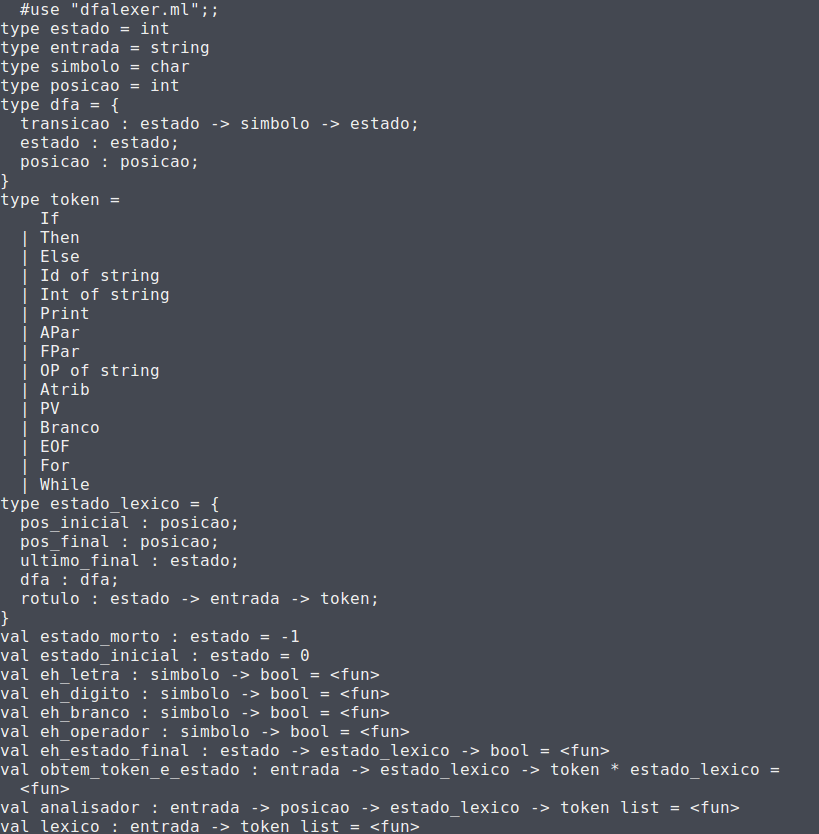
\includegraphics[scale=0.5]{Figures/lexico0}
	\end{figure}
	\newpage
	
	\noindent\textbf{\large Palavras Reservadas}
	
	Foram testadas as palavras reservadas \textbf{if, then, else, print, for e while}. Percebe-se que o autômato também pega espaços em branco.
	
	\begin{figure}[!h]
		\centering
		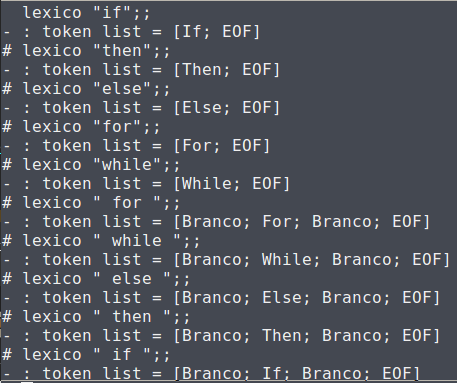
\includegraphics[scale=0.5]{Figures/lexico1}
	\end{figure}
	
	\noindent\textbf{\large Identificadores e Números inteiros}
	
	\begin{figure}[!h]
		\centering
		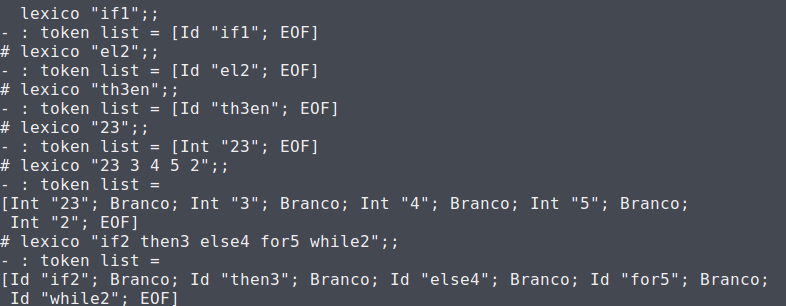
\includegraphics[scale=0.5]{Figures/lexico2}
	\end{figure}
	
	\noindent\textbf{\large Operadores, Atribuição, Ponto e Vírgula e Parênteses}
	
	Repare que o autômato não reconhece o sinal de $=$ como atribuição. Ele somente reconhece $:=$  .
	
	\begin{figure}[!h]
		\centering
		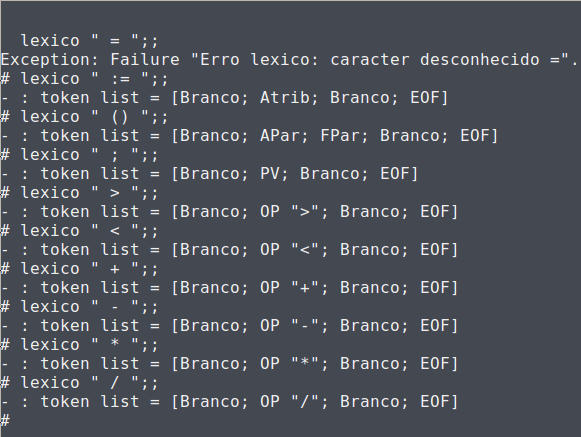
\includegraphics[scale=0.5]{Figures/lexico3}
	\end{figure}
	
	\noindent\textbf{\large Comentários}
	
	Convecionou-se que os comentários serão determinados por $\sharp\sharp$ em virtude da proximidade com Python.
	
	\begin{figure}[!h]
		\centering
		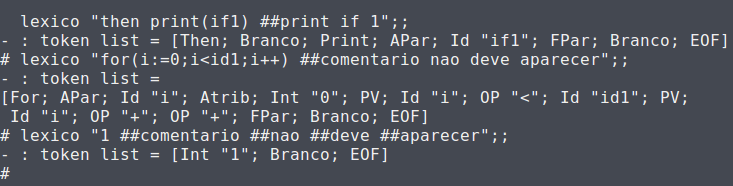
\includegraphics[scale=0.5]{Figures/lexico5}
	\end{figure}
	
	\newpage
	\noindent\textbf{\large Exemplos dados em Aula}
	
	Seguem os exemplos que serão testados:
	\begin{enumerate}
		\item \textbf{$i := 1 + b ;$}
		\item \textbf{$print(a*b);$}
		\item \textbf{$if1 := a-2;$}
		\item \textbf{$then$    $print(if1);$}
		\item \textbf{$else$  $print(if2);$}
	\end{enumerate}
	
	\begin{figure}[!h]
		\centering
		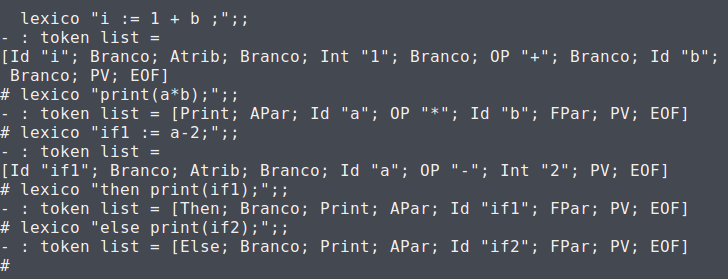
\includegraphics[scale=0.5]{Figures/lexico4}
	\end{figure}
	
	\subsection{Abordagem por Linguagem Regular}
	
	Foi feita uma implementação de linguagem regular em virtude de facilitar o processo de análise léxica.
	
	\subsubsection{Implementação}
	
		Os principais tokens são NOVALINHA, IDENTA e DEDENTA que realizam o controle de identação do python. NOVALINHA é inserido após a quebra de linha e pode ser seguido do identa caso algum comando seja dado. EX.: for, while, ou seja, comandos que exigem identação, O token DEDENTA é utilizado toda a vez a identação volta ao normal o que significa o fim de um comando.
		
		Fazendo uma analogia com a linguagem C, pode-se dizer que o token NOVALINHA representa a vírgula, IDENTA representa abrir chaves e DEDENTA, fechar chaves.
		
		
	\subsubsection{Testes}
	
	
	{\large \textbf{Código} }
		\lstinputlisting{../CodigosTeste/Lexico/nano01.py}	
	
	{\large \textbf{Saída}}
	
	\begin{lstlisting}[caption=Analisador Léxico]
	- : tokens =
	[Lexico.DEF; Lexico.ID "nano01"; Lexico.APAR; Lexico.FPAR; Lexico.DPONTOS;
	Lexico.SETA; Lexico.VOID; Lexico.DPONTOS; Lexico.NOVALINHA; Lexico.INDENTA;
	Lexico.PASS; Lexico.NOVALINHA; Lexico.DEDENTA; Lexico.EOF]


	\end{lstlisting}
	
	{\large \textbf{Código} }
	\lstinputlisting{../CodigosTeste/Lexico/nano02.py}
	
	{\large \textbf{Saída}}
	
	\begin{lstlisting}[caption=Analisador Léxico]
	- : tokens =
	[Lexico.DEF; Lexico.ID "nano02"; Lexico.APAR; Lexico.FPAR; Lexico.DPONTOS;
	Lexico.SETA; Lexico.VOID; Lexico.DPONTOS; Lexico.NOVALINHA; Lexico.INDENTA;
	Lexico.ID "n"; Lexico.ATRIB; Lexico.LITINT 0; Lexico.NOVALINHA;
	Lexico.DEDENTA; Lexico.EOF]
	
	
	\end{lstlisting}
	
	{\large \textbf{Código} }
	\lstinputlisting{../CodigosTeste/Lexico/nano03.py}	
	
	{\large \textbf{Saída}}
	
	\begin{lstlisting}[caption=Analisador Léxico]
	- : tokens =
	[Lexico.DEF; Lexico.ID "nano03"; Lexico.APAR; Lexico.FPAR; Lexico.DPONTOS;
	Lexico.SETA; Lexico.VOID; Lexico.DPONTOS; Lexico.NOVALINHA; Lexico.INDENTA;
	Lexico.ID "n"; Lexico.ATRIB; Lexico.LITINT 1; Lexico.NOVALINHA;
	Lexico.DEDENTA; Lexico.EOF]
	
	
	\end{lstlisting}
	
	{\large \textbf{Código} }
	\lstinputlisting{../CodigosTeste/Lexico/nano04.py}		
	
	{\large \textbf{Saída}}
	
	\begin{lstlisting}[caption=Analisador Léxico]

	- : tokens =
	[Lexico.DEF; Lexico.ID "nano04"; Lexico.APAR; Lexico.FPAR; Lexico.DPONTOS;
	Lexico.SETA; Lexico.VOID; Lexico.DPONTOS; Lexico.NOVALINHA; Lexico.INDENTA;
	Lexico.ID "n"; Lexico.ATRIB; Lexico.LITINT 1; Lexico.MAIS; Lexico.LITINT 2;
	Lexico.NOVALINHA; Lexico.DEDENTA; Lexico.EOF]
	
	\end{lstlisting}
	
	{\large \textbf{Código} }
	\lstinputlisting{../CodigosTeste/Lexico/nano05.py}		
	
	{\large \textbf{Saída}}
	
	\begin{lstlisting}[caption=Analisador Léxico]
	- : tokens =
	[Lexico.DEF; Lexico.ID "nano05"; Lexico.APAR; Lexico.FPAR; Lexico.DPONTOS;
	Lexico.SETA; Lexico.VOID; Lexico.DPONTOS; Lexico.NOVALINHA; Lexico.INDENTA;
	Lexico.ID "n"; Lexico.ATRIB; Lexico.LITINT 2; Lexico.NOVALINHA;
	Lexico.PRINT; Lexico.APAR; Lexico.ID "n"; Lexico.FPAR; Lexico.NOVALINHA;
	Lexico.DEDENTA; Lexico.ID "nano05"; Lexico.APAR; Lexico.FPAR;
	Lexico.NOVALINHA; Lexico.EOF]
	\end{lstlisting}
	
	{\large \textbf{Código} }
	\lstinputlisting{../CodigosTeste/Lexico/nano06.py}		
	
	{\large \textbf{Saída}}
	
	\begin{lstlisting}[caption=Analisador Léxico]
	- : tokens =
	[Lexico.DEF; Lexico.ID "nano06"; Lexico.APAR; Lexico.FPAR; Lexico.DPONTOS;
	Lexico.SETA; Lexico.VOID; Lexico.DPONTOS; Lexico.NOVALINHA; Lexico.INDENTA;
	Lexico.ID "n"; Lexico.ATRIB; Lexico.LITINT 1; Lexico.MENOS; Lexico.LITINT 2;
	Lexico.NOVALINHA; Lexico.PRINT; Lexico.APAR; Lexico.ID "n"; Lexico.FPAR;
	Lexico.NOVALINHA; Lexico.DEDENTA; Lexico.ID "nano06"; Lexico.APAR;
	Lexico.FPAR; Lexico.NOVALINHA; Lexico.EOF]
	
	\end{lstlisting}
	
	{\large \textbf{Código} }
	\lstinputlisting{../CodigosTeste/Lexico/nano07.py}		
	
	{\large \textbf{Saída}}
	
	\begin{lstlisting}[caption=Analisador Léxico]
	- : tokens =
	[Lexico.DEF; Lexico.ID "nano07"; Lexico.APAR; Lexico.FPAR; Lexico.DPONTOS;
	Lexico.SETA; Lexico.VOID; Lexico.DPONTOS; Lexico.NOVALINHA; Lexico.INDENTA;
	Lexico.ID "n"; Lexico.ATRIB; Lexico.LITINT 1; Lexico.NOVALINHA; Lexico.IF;
	Lexico.ID "n"; Lexico.IGUALDADE; Lexico.LITINT 1; Lexico.DPONTOS;
	Lexico.NOVALINHA; Lexico.INDENTA; Lexico.PRINT; Lexico.APAR; Lexico.ID "n";
	Lexico.FPAR; Lexico.NOVALINHA; Lexico.DEDENTA; Lexico.DEDENTA;
	Lexico.ID "nano07"; Lexico.APAR; Lexico.FPAR; Lexico.NOVALINHA; Lexico.EOF]
	
	
	\end{lstlisting}
	
	{\large \textbf{Código} }
	\lstinputlisting{../CodigosTeste/Lexico/nano08.py}		
	
	{\large \textbf{Saída}}
	
	\begin{lstlisting}[caption=Analisador Léxico]
	- : tokens =
	[Lexico.DEF; Lexico.ID "nano08"; Lexico.APAR; Lexico.FPAR; Lexico.DPONTOS;
	Lexico.SETA; Lexico.VOID; Lexico.DPONTOS; Lexico.NOVALINHA; Lexico.INDENTA;
	Lexico.ID "n"; Lexico.ATRIB; Lexico.LITINT 1; Lexico.NOVALINHA; Lexico.IF;
	Lexico.ID "n"; Lexico.IGUALDADE; Lexico.LITINT 1; Lexico.DPONTOS;
	Lexico.NOVALINHA; Lexico.INDENTA; Lexico.PRINT; Lexico.APAR; Lexico.ID "n";
	Lexico.FPAR; Lexico.NOVALINHA; Lexico.DEDENTA; Lexico.ELSE; Lexico.DPONTOS;
	Lexico.NOVALINHA; Lexico.INDENTA; Lexico.PRINT; Lexico.APAR;
	Lexico.LITINT 0; Lexico.FPAR; Lexico.NOVALINHA; Lexico.DEDENTA;
	Lexico.DEDENTA; Lexico.ID "nano08"; Lexico.APAR; Lexico.FPAR;
	Lexico.NOVALINHA; Lexico.EOF]
	\end{lstlisting}
	
	{\large \textbf{Código} }
	\lstinputlisting{../CodigosTeste/Lexico/nano10.py}		
	
	{\large \textbf{Saída}}
	
	\begin{lstlisting}[caption=Analisador Léxico]
	- : tokens =
	[Lexico.DEF; Lexico.ID "nano10"; Lexico.APAR; Lexico.FPAR; Lexico.DPONTOS;
	Lexico.SETA; Lexico.VOID; Lexico.DPONTOS; Lexico.NOVALINHA; Lexico.INDENTA;
	Lexico.ID "n"; Lexico.ATRIB; Lexico.LITINT 1; Lexico.NOVALINHA;
	Lexico.ID "m"; Lexico.ATRIB; Lexico.LITINT 2; Lexico.NOVALINHA; Lexico.IF;
	Lexico.ID "n"; Lexico.IGUALDADE; Lexico.ID "m"; Lexico.DPONTOS;
	Lexico.NOVALINHA; Lexico.INDENTA; Lexico.PRINT; Lexico.APAR; Lexico.ID "n";
	Lexico.FPAR; Lexico.NOVALINHA; Lexico.DEDENTA; Lexico.ELSE; Lexico.DPONTOS;
	Lexico.NOVALINHA; Lexico.INDENTA; Lexico.PRINT; Lexico.APAR;
	Lexico.LITINT 0; Lexico.FPAR; Lexico.NOVALINHA; Lexico.DEDENTA;
	Lexico.DEDENTA; Lexico.ID "nano10"; Lexico.APAR; Lexico.FPAR;
	Lexico.NOVALINHA; Lexico.EOF]
	\end{lstlisting}
	
	{\large \textbf{Código} }
	\lstinputlisting{../CodigosTeste/Lexico/nano11.py}		
	
	{\large \textbf{Saída}}
	
	\begin{lstlisting}[caption=Analisador Léxico]
	- : tokens =
	[Lexico.DEF; Lexico.ID "nano11"; Lexico.APAR; Lexico.FPAR; Lexico.DPONTOS;
	Lexico.SETA; Lexico.VOID; Lexico.DPONTOS; Lexico.NOVALINHA; Lexico.INDENTA;
	Lexico.ID "n"; Lexico.ATRIB; Lexico.LITINT 1; Lexico.NOVALINHA;
	Lexico.ID "m"; Lexico.ATRIB; Lexico.LITINT 2; Lexico.NOVALINHA;
	Lexico.ID "x"; Lexico.ATRIB; Lexico.LITINT 5; Lexico.NOVALINHA;
	Lexico.WHILE; Lexico.ID "x"; Lexico.MAIOR; Lexico.ID "n"; Lexico.DPONTOS;
	Lexico.NOVALINHA; Lexico.INDENTA; Lexico.ID "n"; Lexico.ATRIB;
	Lexico.ID "n"; Lexico.MAIS; Lexico.ID "m"; Lexico.NOVALINHA; Lexico.PRINT;
	Lexico.APAR; Lexico.ID "n"; Lexico.FPAR; Lexico.NOVALINHA; Lexico.DEDENTA;
	Lexico.DEDENTA; Lexico.ID "nano11"; Lexico.APAR; Lexico.FPAR;
	Lexico.NOVALINHA; Lexico.EOF]
	\end{lstlisting}
	
	{\large \textbf{Código} }
	\lstinputlisting{../CodigosTeste/Lexico/nano12.py}		
	
	{\large \textbf{Saída}}
	
	\begin{lstlisting}[caption=Analisador Léxico]
	- : tokens =
	[Lexico.DEF; Lexico.ID "nano12"; Lexico.APAR; Lexico.FPAR; Lexico.DPONTOS;
	Lexico.SETA; Lexico.VOID; Lexico.DPONTOS; Lexico.NOVALINHA; Lexico.INDENTA;
	Lexico.ID "n"; Lexico.ATRIB; Lexico.LITINT 1; Lexico.NOVALINHA;
	Lexico.ID "m"; Lexico.ATRIB; Lexico.LITINT 2; Lexico.NOVALINHA;
	Lexico.ID "x"; Lexico.ATRIB; Lexico.LITINT 5; Lexico.NOVALINHA;
	Lexico.WHILE; Lexico.ID "x"; Lexico.MAIOR; Lexico.ID "n"; Lexico.DPONTOS;
	Lexico.NOVALINHA; Lexico.INDENTA; Lexico.IF; Lexico.ID "n";
	Lexico.IGUALDADE; Lexico.ID "m"; Lexico.DPONTOS; Lexico.NOVALINHA;
	Lexico.INDENTA; Lexico.PRINT; Lexico.APAR; Lexico.ID "n"; Lexico.FPAR;
	Lexico.NOVALINHA; Lexico.DEDENTA; Lexico.ELSE; Lexico.DPONTOS;
	Lexico.NOVALINHA; Lexico.INDENTA; Lexico.PRINT; Lexico.APAR;
	Lexico.LITINT 0; Lexico.FPAR; Lexico.NOVALINHA; Lexico.DEDENTA;
	Lexico.ID "x"; Lexico.ATRIB; Lexico.ID "x"; Lexico.MENOS; Lexico.LITINT 1;
	Lexico.NOVALINHA; Lexico.DEDENTA; Lexico.DEDENTA; Lexico.ID "nano12";
	Lexico.APAR; Lexico.FPAR; Lexico.NOVALINHA; Lexico.EOF]
	\end{lstlisting}
	
	{\large \textbf{Código} }
	\lstinputlisting{../CodigosTeste/Lexico/micro01.py}		
	
	{\large \textbf{Saída}}
	
	\begin{lstlisting}[caption=Analisador Léxico]
	- : tokens =
	[Lexico.DEF; Lexico.ID "micro01"; Lexico.APAR; Lexico.FPAR; Lexico.DPONTOS;
	Lexico.SETA; Lexico.VOID; Lexico.DPONTOS; Lexico.NOVALINHA; Lexico.INDENTA;
	Lexico.ID "cel"; Lexico.VIRG; Lexico.ID "far"; Lexico.ATRIB;
	Lexico.LITINT 1; Lexico.PONTO; Lexico.LITINT 0; Lexico.VIRG;
	Lexico.LITINT 0; Lexico.PONTO; Lexico.LITINT 0; Lexico.NOVALINHA;
	Lexico.PRINT; Lexico.APAR;
	Lexico.LITSTRING "\t\tTabela de conversao: Celsius -> Fahrenheit";
	Lexico.FPAR; Lexico.NOVALINHA; Lexico.PRINT; Lexico.APAR;
	Lexico.LITSTRING "Digite a temperatura em Celsius: "; Lexico.FPAR;
	Lexico.NOVALINHA; Lexico.ID "cel"; Lexico.ATRIB; Lexico.INPUT; Lexico.APAR;
	Lexico.FPAR; Lexico.NOVALINHA; Lexico.ID "far"; Lexico.ATRIB; Lexico.APAR;
	Lexico.LITINT 9; Lexico.VEZES; Lexico.ID "cel"; Lexico.MAIS;
	Lexico.LITINT 160; Lexico.FPAR; Lexico.DIVIDIDO; Lexico.LITINT 5;
	Lexico.NOVALINHA; Lexico.PRINT; Lexico.APAR;
	Lexico.LITSTRING "A nova temperatura e:"; Lexico.MAIS; Lexico.STR;
	Lexico.APAR; Lexico.ID "far"; Lexico.FPAR; Lexico.MAIS;
	Lexico.LITSTRING "F"; Lexico.FPAR; Lexico.NOVALINHA; Lexico.NOVALINHA;
	Lexico.DEDENTA; Lexico.EOF]
	\end{lstlisting}
	
	
	{\large \textbf{Código} }
	\lstinputlisting{../CodigosTeste/Lexico/micro02.py}		
	
	{\large \textbf{Saída}}
	
	\begin{lstlisting}[caption=Analisador Léxico]
	- : tokens =
	[Lexico.DEF; Lexico.ID "micro02"; Lexico.APAR; Lexico.FPAR; Lexico.DPONTOS;
	Lexico.SETA; Lexico.VOID; Lexico.DPONTOS; Lexico.NOVALINHA; Lexico.INDENTA;
	Lexico.ID "num1"; Lexico.VIRG; Lexico.ID "num2"; Lexico.ATRIB;
	Lexico.LITINT 0; Lexico.VIRG; Lexico.LITINT 0; Lexico.NOVALINHA;
	Lexico.PRINT; Lexico.APAR; Lexico.LITSTRING "Digite o primeiro numero: ";
	Lexico.FPAR; Lexico.NOVALINHA; Lexico.ID "num1"; Lexico.ATRIB; Lexico.INT;
	Lexico.APAR; Lexico.INPUT; Lexico.APAR; Lexico.FPAR; Lexico.FPAR;
	Lexico.NOVALINHA; Lexico.PRINT; Lexico.APAR;
	Lexico.LITSTRING "Digite o segundo numero: "; Lexico.FPAR; Lexico.NOVALINHA;
	Lexico.ID "num2"; Lexico.ATRIB; Lexico.INT; Lexico.APAR; Lexico.INPUT;
	Lexico.APAR; Lexico.FPAR; Lexico.FPAR; Lexico.NOVALINHA; Lexico.IF;
	Lexico.ID "num1"; Lexico.MAIOR; Lexico.ID "num2"; Lexico.DPONTOS;
	Lexico.NOVALINHA; Lexico.INDENTA; Lexico.PRINT; Lexico.APAR;
	Lexico.LITSTRING "O primeiro numero "; Lexico.MAIS; Lexico.STR; Lexico.APAR;
	Lexico.ID "num1"; Lexico.FPAR; Lexico.MAIS;
	Lexico.LITSTRING " e maior que o segundo "; Lexico.MAIS; Lexico.STR;
	Lexico.APAR; Lexico.ID "num2"; Lexico.FPAR; Lexico.FPAR; Lexico.NOVALINHA;
	Lexico.DEDENTA; Lexico.ELSE; Lexico.DPONTOS; Lexico.NOVALINHA;
	Lexico.INDENTA; Lexico.PRINT; Lexico.APAR;
	Lexico.LITSTRING "O segundo numero "; Lexico.MAIS; Lexico.STR; Lexico.APAR;
	Lexico.ID "num2"; Lexico.FPAR; Lexico.MAIS;
	Lexico.LITSTRING " e maior que o primeiro "; Lexico.MAIS; Lexico.STR;
	Lexico.APAR; Lexico.ID "num1"; Lexico.FPAR; Lexico.FPAR; Lexico.NOVALINHA;
	Lexico.DEDENTA; Lexico.DEDENTA; Lexico.ID "micro02"; Lexico.APAR;
	Lexico.FPAR; Lexico.NOVALINHA; Lexico.EOF]
	\end{lstlisting}
	
	
	{\large \textbf{Código} }
	\lstinputlisting{../CodigosTeste/Lexico/micro03.py}		
	
	{\large \textbf{Saída}}
	
	\begin{lstlisting}[caption=Analisador Léxico]
	- : tokens =
	[Lexico.DEF; Lexico.ID "micro03"; Lexico.APAR; Lexico.FPAR; Lexico.DPONTOS;
	Lexico.SETA; Lexico.VOID; Lexico.DPONTOS; Lexico.NOVALINHA; Lexico.INDENTA;
	Lexico.ID "numero"; Lexico.ATRIB; Lexico.LITINT 0; Lexico.NOVALINHA;
	Lexico.PRINT; Lexico.APAR; Lexico.LITSTRING "Digite um numero: ";
	Lexico.FPAR; Lexico.NOVALINHA; Lexico.ID "numero"; Lexico.ATRIB; Lexico.INT;
	Lexico.APAR; Lexico.INPUT; Lexico.APAR; Lexico.FPAR; Lexico.FPAR;
	Lexico.NOVALINHA; Lexico.IF; Lexico.ID "numero"; Lexico.MAIORIGUAL;
	Lexico.LITINT 100; Lexico.DPONTOS; Lexico.NOVALINHA; Lexico.INDENTA;
	Lexico.IF; Lexico.ID "numero"; Lexico.MENORIGUAL; Lexico.LITINT 200;
	Lexico.DPONTOS; Lexico.NOVALINHA; Lexico.INDENTA; Lexico.PRINT; Lexico.APAR;
	Lexico.LITSTRING "O numero esta no intervalo entre 100 e 200"; Lexico.FPAR;
	Lexico.NOVALINHA; Lexico.DEDENTA; Lexico.ELSE; Lexico.DPONTOS;
	Lexico.NOVALINHA; Lexico.INDENTA; Lexico.PRINT; Lexico.APAR;
	Lexico.LITSTRING "O numero nao esta no intervalo entre 100 e 200";
	Lexico.FPAR; Lexico.NOVALINHA; Lexico.DEDENTA; Lexico.DEDENTA; Lexico.ELSE;
	Lexico.DPONTOS; Lexico.NOVALINHA; Lexico.INDENTA; Lexico.PRINT; Lexico.APAR;
	Lexico.LITSTRING "O numero nao esta no intervalo entre 100 e 200";
	Lexico.FPAR; Lexico.NOVALINHA; Lexico.DEDENTA; Lexico.DEDENTA;
	Lexico.ID "micro03"; Lexico.APAR; Lexico.FPAR; Lexico.NOVALINHA; Lexico.EOF]
	\end{lstlisting}
	
	
	{\large \textbf{Código} }
	\lstinputlisting{../CodigosTeste/Lexico/micro04.py}		
	
	{\large \textbf{Saída}}
	
	\begin{lstlisting}[caption=Analisador Léxico]
	- : tokens =
	[Lexico.DEF; Lexico.ID "micro04"; Lexico.APAR; Lexico.FPAR; Lexico.DPONTOS;
	Lexico.SETA; Lexico.VOID; Lexico.DPONTOS; Lexico.NOVALINHA; Lexico.INDENTA;
	Lexico.ID "x"; Lexico.VIRG; Lexico.ID "num"; Lexico.VIRG;
	Lexico.ID "intervalo"; Lexico.ATRIB; Lexico.LITINT 0; Lexico.VIRG;
	Lexico.LITINT 0; Lexico.VIRG; Lexico.LITINT 0; Lexico.NOVALINHA; Lexico.FOR;
	Lexico.ID "x"; Lexico.IN; Lexico.RANGE; Lexico.APAR; Lexico.LITINT 5;
	Lexico.FPAR; Lexico.DPONTOS; Lexico.NOVALINHA; Lexico.INDENTA; Lexico.PRINT;
	Lexico.APAR; Lexico.LITSTRING "Digite o numero: "; Lexico.FPAR;
	Lexico.NOVALINHA; Lexico.ID "num"; Lexico.ATRIB; Lexico.INT; Lexico.APAR;
	Lexico.INPUT; Lexico.APAR; Lexico.FPAR; Lexico.FPAR; Lexico.NOVALINHA;
	Lexico.IF; Lexico.ID "num"; Lexico.MAIORIGUAL; Lexico.LITINT 10;
	Lexico.DPONTOS; Lexico.NOVALINHA; Lexico.INDENTA; Lexico.IF;
	Lexico.ID "num"; Lexico.MENORIGUAL; Lexico.LITINT 150; Lexico.DPONTOS;
	Lexico.NOVALINHA; Lexico.INDENTA; Lexico.ID "intervalo"; Lexico.ATRIB;
	Lexico.ID "intervalo"; Lexico.MAIS; Lexico.LITINT 1; Lexico.NOVALINHA;
	Lexico.DEDENTA; Lexico.DEDENTA; Lexico.DEDENTA; Lexico.PRINT; Lexico.APAR;
	Lexico.LITSTRING "Ao total, foram digitados "; Lexico.MAIS; Lexico.STR;
	Lexico.APAR; Lexico.ID "intervalo"; Lexico.FPAR; Lexico.MAIS;
	Lexico.LITSTRING " numeros no intervalo entre 10 e 150"; Lexico.FPAR;
	Lexico.NOVALINHA; Lexico.DEDENTA; Lexico.ID "micro04"; Lexico.APAR;
	Lexico.FPAR; Lexico.NOVALINHA; Lexico.EOF]
	\end{lstlisting}
	
	
	{\large \textbf{Código} }
	\lstinputlisting{../CodigosTeste/Lexico/micro05.py}		
	
	{\large \textbf{Saída}}
	
	\begin{lstlisting}[caption=Analisador Léxico]
	- : tokens =
	[Lexico.DEF; Lexico.ID "micro05"; Lexico.APAR; Lexico.FPAR; Lexico.DPONTOS;
	Lexico.SETA; Lexico.VOID; Lexico.DPONTOS; Lexico.NOVALINHA; Lexico.INDENTA;
	Lexico.ID "x"; Lexico.VIRG; Lexico.ID "h"; Lexico.VIRG; Lexico.ID "h";
	Lexico.ATRIB; Lexico.LITINT 0; Lexico.VIRG; Lexico.LITINT 0; Lexico.VIRG;
	Lexico.LITINT 0; Lexico.NOVALINHA; Lexico.ID "nome"; Lexico.VIRG;
	Lexico.ID "sexo"; Lexico.ATRIB; Lexico.LITSTRING ""; Lexico.VIRG;
	Lexico.LITSTRING ""; Lexico.NOVALINHA; Lexico.FOR; Lexico.ID "x"; Lexico.IN;
	Lexico.RANGE; Lexico.APAR; Lexico.LITINT 5; Lexico.FPAR; Lexico.DPONTOS;
	Lexico.NOVALINHA; Lexico.INDENTA; Lexico.PRINT; Lexico.APAR;
	Lexico.LITSTRING "Digite o nome: "; Lexico.FPAR; Lexico.NOVALINHA;
	Lexico.ID "nome"; Lexico.ATRIB; Lexico.INPUT; Lexico.APAR; Lexico.FPAR;
	Lexico.NOVALINHA; Lexico.PRINT; Lexico.APAR;
	Lexico.LITSTRING "H - Homem ou M - Mulher"; Lexico.FPAR; Lexico.NOVALINHA;
	Lexico.ID "sexo"; Lexico.ATRIB; Lexico.INPUT; Lexico.APAR; Lexico.FPAR;
	Lexico.NOVALINHA; Lexico.IF; Lexico.ID "sexo"; Lexico.IGUALDADE;
	Lexico.LITSTRING "H"; Lexico.DPONTOS; Lexico.NOVALINHA; Lexico.INDENTA;
	Lexico.ID "h"; Lexico.ATRIB; Lexico.ID "h"; Lexico.MAIS; Lexico.LITINT 1;
	Lexico.NOVALINHA; Lexico.DEDENTA; Lexico.ELIF; Lexico.ID "sexo";
	Lexico.IGUALDADE; Lexico.LITSTRING "M"; Lexico.DPONTOS; Lexico.NOVALINHA;
	Lexico.INDENTA; Lexico.ID "m"; Lexico.ATRIB; Lexico.ID "m"; Lexico.MAIS;
	Lexico.LITINT 1; Lexico.NOVALINHA; Lexico.DEDENTA; Lexico.ELSE;
	Lexico.DPONTOS; Lexico.NOVALINHA; Lexico.INDENTA; Lexico.PRINT; Lexico.APAR;
	Lexico.LITSTRING "Sexo so pode ser H ou M!"; Lexico.FPAR; Lexico.NOVALINHA;
	Lexico.DEDENTA; Lexico.DEDENTA; Lexico.PRINT; Lexico.APAR;
	Lexico.LITSTRING "Foram inseridos "; Lexico.MAIS; Lexico.ID "h";
	Lexico.MAIS; Lexico.LITSTRING " Homens"; Lexico.FPAR; Lexico.NOVALINHA;
	Lexico.PRINT; Lexico.APAR; Lexico.LITSTRING "Foram inseridas "; Lexico.MAIS;
	Lexico.ID "m"; Lexico.MAIS; Lexico.LITSTRING " Mulheres"; Lexico.FPAR;
	Lexico.NOVALINHA; Lexico.DEDENTA; Lexico.ID "micro05"; Lexico.APAR;
	Lexico.FPAR; Lexico.NOVALINHA; Lexico.EOF]
	\end{lstlisting}
	
	
	{\large \textbf{Código} }
	\lstinputlisting{../CodigosTeste/Lexico/micro06.py}		
	
	{\large \textbf{Saída}}
	
	\begin{lstlisting}[caption=Analisador Léxico]
	- : tokens =
	[Lexico.DEF; Lexico.ID "micro06"; Lexico.APAR; Lexico.FPAR; Lexico.DPONTOS;
	Lexico.SETA; Lexico.VOID; Lexico.DPONTOS; Lexico.NOVALINHA; Lexico.INDENTA;
	Lexico.ID "numero"; Lexico.ATRIB; Lexico.LITINT 0; Lexico.NOVALINHA;
	Lexico.PRINT; Lexico.APAR; Lexico.LITSTRING "Digite um numero de 1 a 5: ";
	Lexico.FPAR; Lexico.NOVALINHA; Lexico.ID "numero"; Lexico.ATRIB; Lexico.INT;
	Lexico.APAR; Lexico.INPUT; Lexico.APAR; Lexico.FPAR; Lexico.FPAR;
	Lexico.NOVALINHA; Lexico.IF; Lexico.ID "numero"; Lexico.IGUALDADE;
	Lexico.LITINT 1; Lexico.DPONTOS; Lexico.NOVALINHA; Lexico.INDENTA;
	Lexico.PRINT; Lexico.APAR; Lexico.LITSTRING "Um"; Lexico.FPAR;
	Lexico.NOVALINHA; Lexico.DEDENTA; Lexico.ELIF; Lexico.ID "numero";
	Lexico.IGUALDADE; Lexico.LITINT 2; Lexico.DPONTOS; Lexico.NOVALINHA;
	Lexico.INDENTA; Lexico.PRINT; Lexico.APAR; Lexico.LITSTRING "Dois";
	Lexico.FPAR; Lexico.NOVALINHA; Lexico.DEDENTA; Lexico.ELIF;
	Lexico.ID "numero"; Lexico.IGUALDADE; Lexico.LITINT 3; Lexico.DPONTOS;
	Lexico.NOVALINHA; Lexico.INDENTA; Lexico.PRINT; Lexico.APAR;
	Lexico.LITSTRING "Tres"; Lexico.FPAR; Lexico.NOVALINHA; Lexico.DEDENTA;
	Lexico.ELIF; Lexico.ID "numero"; Lexico.IGUALDADE; Lexico.LITINT 4;
	Lexico.DPONTOS; Lexico.NOVALINHA; Lexico.INDENTA; Lexico.PRINT; Lexico.APAR;
	Lexico.LITSTRING "Quatro"; Lexico.FPAR; Lexico.NOVALINHA; Lexico.DEDENTA;
	Lexico.ELIF; Lexico.ID "numero"; Lexico.IGUALDADE; Lexico.LITINT 5;
	Lexico.DPONTOS; Lexico.NOVALINHA; Lexico.INDENTA; Lexico.PRINT; Lexico.APAR;
	Lexico.LITSTRING "Cinco"; Lexico.FPAR; Lexico.NOVALINHA; Lexico.DEDENTA;
	Lexico.ELSE; Lexico.DPONTOS; Lexico.NOVALINHA; Lexico.INDENTA; Lexico.PRINT;
	Lexico.APAR; Lexico.LITSTRING "Numero Invalido!!!"; Lexico.FPAR;
	Lexico.NOVALINHA; Lexico.DEDENTA; Lexico.DEDENTA; Lexico.ID "micro06";
	Lexico.APAR; Lexico.FPAR; Lexico.NOVALINHA; Lexico.EOF]
	\end{lstlisting}
	
	
	{\large \textbf{Código} }
	\lstinputlisting{../CodigosTeste/Lexico/micro07.py}		
	
	{\large \textbf{Saída}}
	
	\begin{lstlisting}[caption=Analisador Léxico]
	- : tokens =
	[Lexico.DEF; Lexico.ID "micro07"; Lexico.APAR; Lexico.FPAR; Lexico.DPONTOS;
	Lexico.SETA; Lexico.VOID; Lexico.DPONTOS; Lexico.NOVALINHA; Lexico.INDENTA;
	Lexico.ID "numero"; Lexico.VIRG; Lexico.ID "programa"; Lexico.ATRIB;
	Lexico.LITINT 0; Lexico.VIRG; Lexico.LITINT 1; Lexico.NOVALINHA;
	Lexico.ID "opc"; Lexico.ATRIB; Lexico.LITSTRING ""; Lexico.NOVALINHA;
	Lexico.WHILE; Lexico.ID "programa"; Lexico.IGUALDADE; Lexico.LITINT 1;
	Lexico.DPONTOS; Lexico.NOVALINHA; Lexico.INDENTA; Lexico.PRINT; Lexico.APAR;
	Lexico.LITSTRING "Digite um numero: "; Lexico.FPAR; Lexico.NOVALINHA;
	Lexico.ID "numero"; Lexico.ATRIB; Lexico.INT; Lexico.APAR; Lexico.INPUT;
	Lexico.APAR; Lexico.FPAR; Lexico.FPAR; Lexico.NOVALINHA; Lexico.IF;
	Lexico.ID "numero"; Lexico.MAIOR; Lexico.LITINT 0; Lexico.DPONTOS;
	Lexico.NOVALINHA; Lexico.INDENTA; Lexico.PRINT; Lexico.APAR;
	Lexico.LITSTRING "Positivo"; Lexico.FPAR; Lexico.NOVALINHA; Lexico.DEDENTA;
	Lexico.ELSE; Lexico.DPONTOS; Lexico.NOVALINHA; Lexico.INDENTA; Lexico.IF;
	Lexico.ID "numero"; Lexico.IGUALDADE; Lexico.LITINT 0; Lexico.DPONTOS;
	Lexico.NOVALINHA; Lexico.INDENTA; Lexico.PRINT; Lexico.APAR;
	Lexico.LITSTRING "O numero e igual a 0"; Lexico.FPAR; Lexico.NOVALINHA;
	Lexico.DEDENTA; Lexico.IF; Lexico.ID "numero"; Lexico.MENOR;
	Lexico.LITINT 0; Lexico.DPONTOS; Lexico.NOVALINHA; Lexico.INDENTA;
	Lexico.PRINT; Lexico.APAR; Lexico.LITSTRING "Negativo"; Lexico.FPAR;
	Lexico.NOVALINHA; Lexico.DEDENTA; Lexico.DEDENTA; Lexico.PRINT; Lexico.APAR;
	Lexico.LITSTRING "Deseja Finalizar? (S/N) "; Lexico.FPAR; Lexico.NOVALINHA;
	Lexico.ID "opc"; Lexico.ATRIB; Lexico.INPUT; Lexico.APAR; Lexico.FPAR;
	Lexico.NOVALINHA; Lexico.IF; Lexico.ID "opc"; Lexico.IGUALDADE;
	Lexico.LITSTRING "S"; Lexico.DPONTOS; Lexico.NOVALINHA; Lexico.INDENTA;
	Lexico.ID "programa"; Lexico.ATRIB; Lexico.LITINT 0; Lexico.NOVALINHA;
	Lexico.DEDENTA; Lexico.DEDENTA; Lexico.DEDENTA; Lexico.ID "micro07";
	Lexico.APAR; Lexico.FPAR; Lexico.NOVALINHA; Lexico.EOF]
	\end{lstlisting}
	
	
	{\large \textbf{Código} }
	\lstinputlisting{../CodigosTeste/Lexico/micro08.py}		
	
	{\large \textbf{Saída}}
	
	\begin{lstlisting}[caption=Analisador Léxico]
	- : tokens =
	[Lexico.DEF; Lexico.ID "micro08"; Lexico.APAR; Lexico.FPAR; Lexico.DPONTOS;
	Lexico.SETA; Lexico.VOID; Lexico.DPONTOS; Lexico.NOVALINHA; Lexico.INDENTA;
	Lexico.ID "numero"; Lexico.ATRIB; Lexico.LITINT 1; Lexico.NOVALINHA;
	Lexico.WHILE; Lexico.ID "numero"; Lexico.MENOR; Lexico.LITINT 0; Lexico.OU;
	Lexico.ID "numero"; Lexico.MAIOR; Lexico.LITINT 0; Lexico.DPONTOS;
	Lexico.NOVALINHA; Lexico.INDENTA; Lexico.PRINT; Lexico.APAR;
	Lexico.LITSTRING "Digite o numero"; Lexico.FPAR; Lexico.NOVALINHA;
	Lexico.ID "numero"; Lexico.ATRIB; Lexico.INT; Lexico.APAR; Lexico.INPUT;
	Lexico.APAR; Lexico.FPAR; Lexico.FPAR; Lexico.NOVALINHA; Lexico.IF;
	Lexico.ID "numero"; Lexico.MAIOR; Lexico.LITINT 10; Lexico.DPONTOS;
	Lexico.NOVALINHA; Lexico.INDENTA; Lexico.PRINT; Lexico.APAR;
	Lexico.LITSTRING "O numero "; Lexico.MAIS; Lexico.STR; Lexico.APAR;
	Lexico.ID "numero"; Lexico.FPAR; Lexico.MAIS;
	Lexico.LITSTRING " e maior que 10"; Lexico.FPAR; Lexico.NOVALINHA;
	Lexico.DEDENTA; Lexico.ELSE; Lexico.DPONTOS; Lexico.NOVALINHA;
	Lexico.INDENTA; Lexico.PRINT; Lexico.APAR; Lexico.LITSTRING "O numero ";
	Lexico.MAIS; Lexico.STR; Lexico.APAR; Lexico.ID "numero"; Lexico.FPAR;
	Lexico.MAIS; Lexico.LITSTRING " e menor que 10"; Lexico.FPAR;
	Lexico.NOVALINHA; Lexico.DEDENTA; Lexico.DEDENTA; Lexico.DEDENTA;
	Lexico.ID "micro08"; Lexico.APAR; Lexico.FPAR; Lexico.NOVALINHA; Lexico.EOF]
	\end{lstlisting}
	
	
	{\large \textbf{Código} }
	\lstinputlisting{../CodigosTeste/Lexico/micro09.py}		
	
	{\large \textbf{Saída}}
	
	\begin{lstlisting}[caption=Analisador Léxico]
	- : tokens =
	[Lexico.DEF; Lexico.ID "micro09"; Lexico.APAR; Lexico.FPAR; Lexico.DPONTOS;
	Lexico.SETA; Lexico.VOID; Lexico.DPONTOS; Lexico.NOVALINHA; Lexico.INDENTA;
	Lexico.ID "preco"; Lexico.VIRG; Lexico.ID "venda"; Lexico.VIRG;
	Lexico.ID "novopreco"; Lexico.ATRIB; Lexico.LITINT 0; Lexico.PONTO;
	Lexico.LITINT 0; Lexico.VIRG; Lexico.LITINT 0; Lexico.PONTO;
	Lexico.LITINT 0; Lexico.VIRG; Lexico.LITINT 0; Lexico.PONTO;
	Lexico.LITINT 0; Lexico.NOVALINHA; Lexico.PRINT; Lexico.APAR;
	Lexico.LITSTRING "Digite o preco: "; Lexico.FPAR; Lexico.NOVALINHA;
	Lexico.ID "preco"; Lexico.ATRIB; Lexico.INT; Lexico.APAR; Lexico.INPUT;
	Lexico.APAR; Lexico.FPAR; Lexico.FPAR; Lexico.NOVALINHA; Lexico.PRINT;
	Lexico.APAR; Lexico.LITSTRING "Digite a venda: "; Lexico.FPAR;
	Lexico.NOVALINHA; Lexico.ID "venda"; Lexico.ATRIB; Lexico.INT; Lexico.APAR;
	Lexico.INPUT; Lexico.APAR; Lexico.FPAR; Lexico.FPAR; Lexico.NOVALINHA;
	Lexico.IF; Lexico.ID "venda"; Lexico.MENOR; Lexico.LITINT 500; Lexico.OU;
	Lexico.ID "preco"; Lexico.MENOR; Lexico.LITINT 30; Lexico.DPONTOS;
	Lexico.NOVALINHA; Lexico.INDENTA; Lexico.ID "novopreco"; Lexico.ATRIB;
	Lexico.ID "preco"; Lexico.MAIS; Lexico.LITINT 10; Lexico.DIVIDIDO;
	Lexico.LITINT 100; Lexico.VEZES; Lexico.ID "preco"; Lexico.NOVALINHA;
	Lexico.DEDENTA; Lexico.ELIF; Lexico.APAR; Lexico.ID "venda";
	Lexico.MAIORIGUAL; Lexico.LITINT 500; Lexico.E; Lexico.ID "venda";
	Lexico.MENOR; Lexico.LITINT 1200; Lexico.FPAR; Lexico.OU; Lexico.APAR;
	Lexico.ID "preco"; Lexico.MAIORIGUAL; Lexico.LITINT 30; Lexico.E;
	Lexico.ID "preco"; Lexico.MENOR; Lexico.LITINT 80; Lexico.FPAR;
	Lexico.DPONTOS; Lexico.NOVALINHA; Lexico.INDENTA; Lexico.ID "novopreco";
	Lexico.ATRIB; Lexico.ID "preco"; Lexico.MAIS; Lexico.LITINT 15;
	Lexico.DIVIDIDO; Lexico.LITINT 100; Lexico.VEZES; Lexico.ID "preco";
	Lexico.NOVALINHA; Lexico.DEDENTA; Lexico.ELIF; Lexico.ID "venda";
	Lexico.MAIORIGUAL; Lexico.LITINT 1200; Lexico.OU; Lexico.ID "preco";
	Lexico.MAIORIGUAL; Lexico.LITINT 80; Lexico.DPONTOS; Lexico.NOVALINHA;
	Lexico.INDENTA; Lexico.ID "novopreco"; Lexico.ATRIB; Lexico.ID "preco";
	Lexico.MENOS; Lexico.LITINT 20; Lexico.DIVIDIDO; Lexico.LITINT 100;
	Lexico.VEZES; Lexico.ID "preco"; Lexico.NOVALINHA; Lexico.DEDENTA;
	Lexico.PRINT; Lexico.APAR; Lexico.LITSTRING "O novo preco e: "; Lexico.MAIS;
	Lexico.STR; Lexico.APAR; Lexico.ID "novopreco"; Lexico.FPAR; Lexico.FPAR;
	Lexico.NOVALINHA; Lexico.DEDENTA; Lexico.ID "micro09"; Lexico.APAR;
	Lexico.FPAR; Lexico.NOVALINHA; Lexico.EOF]
	\end{lstlisting}
	
	
	{\large \textbf{Código} }
	\lstinputlisting{../CodigosTeste/Lexico/micro10.py}		
	
	{\large \textbf{Saída}}
	
	\begin{lstlisting}[caption=Analisador Léxico]
	- : tokens =
	[Lexico.DEF; Lexico.ID "micro10"; Lexico.APAR; Lexico.FPAR; Lexico.DPONTOS;
	Lexico.SETA; Lexico.VOID; Lexico.DPONTOS; Lexico.NOVALINHA; Lexico.INDENTA;
	Lexico.ID "numero"; Lexico.ATRIB; Lexico.LITINT 0; Lexico.NOVALINHA;
	Lexico.ID "fat"; Lexico.ATRIB; Lexico.LITINT 0; Lexico.NOVALINHA;
	Lexico.PRINT; Lexico.APAR; Lexico.LITSTRING "Digite um numero: ";
	Lexico.FPAR; Lexico.NOVALINHA; Lexico.ID "numero"; Lexico.ATRIB; Lexico.INT;
	Lexico.APAR; Lexico.INPUT; Lexico.APAR; Lexico.FPAR; Lexico.FPAR;
	Lexico.NOVALINHA; Lexico.ID "fat"; Lexico.ATRIB; Lexico.ID "fatorial";
	Lexico.APAR; Lexico.ID "numero"; Lexico.FPAR; Lexico.NOVALINHA;
	Lexico.PRINT; Lexico.APAR; Lexico.LITSTRING "O fatorial de "; Lexico.MAIS;
	Lexico.STR; Lexico.APAR; Lexico.ID "numero"; Lexico.FPAR; Lexico.MAIS;
	Lexico.LITSTRING " e "; Lexico.MAIS; Lexico.STR; Lexico.APAR;
	Lexico.ID "fat"; Lexico.FPAR; Lexico.FPAR; Lexico.NOVALINHA; Lexico.DEDENTA;
	Lexico.DEF; Lexico.ID "fatorial"; Lexico.APAR; Lexico.ID "n";
	Lexico.DPONTOS; Lexico.INT; Lexico.FPAR; Lexico.DPONTOS; Lexico.SETA;
	Lexico.INT; Lexico.DPONTOS; Lexico.NOVALINHA; Lexico.INDENTA; Lexico.IF;
	Lexico.ID "n"; Lexico.MENORIGUAL; Lexico.LITINT 0; Lexico.DPONTOS;
	Lexico.NOVALINHA; Lexico.INDENTA; Lexico.RETURN; Lexico.LITINT 1;
	Lexico.NOVALINHA; Lexico.DEDENTA; Lexico.ELSE; Lexico.DPONTOS;
	Lexico.NOVALINHA; Lexico.INDENTA; Lexico.RETURN; Lexico.APAR; Lexico.ID "n";
	Lexico.VEZES; Lexico.ID "fatorial"; Lexico.APAR; Lexico.ID "n";
	Lexico.MENOS; Lexico.LITINT 1; Lexico.FPAR; Lexico.FPAR; Lexico.NOVALINHA;
	Lexico.DEDENTA; Lexico.DEDENTA; Lexico.ID "micro10"; Lexico.APAR;
	Lexico.FPAR; Lexico.NOVALINHA; Lexico.EOF]
	
	\end{lstlisting}
	
	
	{\large \textbf{Código} }
	\lstinputlisting{../CodigosTeste/Lexico/micro11.py}		
	
	{\large \textbf{Saída}}
	
	\begin{lstlisting}[caption=Analisador Léxico]
	- : tokens =
	[Lexico.DEF; Lexico.ID "micro10"; Lexico.APAR; Lexico.FPAR; Lexico.DPONTOS;
	Lexico.SETA; Lexico.VOID; Lexico.DPONTOS; Lexico.NOVALINHA; Lexico.INDENTA;
	Lexico.ID "numero"; Lexico.ATRIB; Lexico.LITINT 0; Lexico.NOVALINHA;
	Lexico.ID "fat"; Lexico.ATRIB; Lexico.LITINT 0; Lexico.NOVALINHA;
	Lexico.PRINT; Lexico.APAR; Lexico.LITSTRING "Digite um numero: ";
	Lexico.FPAR; Lexico.NOVALINHA; Lexico.ID "numero"; Lexico.ATRIB; Lexico.INT;
	Lexico.APAR; Lexico.INPUT; Lexico.APAR; Lexico.FPAR; Lexico.FPAR;
	Lexico.NOVALINHA; Lexico.ID "fat"; Lexico.ATRIB; Lexico.ID "fatorial";
	Lexico.APAR; Lexico.ID "numero"; Lexico.FPAR; Lexico.NOVALINHA;
	Lexico.PRINT; Lexico.APAR; Lexico.LITSTRING "O fatorial de "; Lexico.MAIS;
	Lexico.STR; Lexico.APAR; Lexico.ID "numero"; Lexico.FPAR; Lexico.MAIS;
	Lexico.LITSTRING " e "; Lexico.MAIS; Lexico.STR; Lexico.APAR;
	Lexico.ID "fat"; Lexico.FPAR; Lexico.FPAR; Lexico.NOVALINHA; Lexico.DEDENTA;
	Lexico.DEF; Lexico.ID "fatorial"; Lexico.APAR; Lexico.ID "n";
	Lexico.DPONTOS; Lexico.INT; Lexico.FPAR; Lexico.DPONTOS; Lexico.SETA;
	Lexico.INT; Lexico.DPONTOS; Lexico.NOVALINHA; Lexico.INDENTA; Lexico.IF;
	Lexico.ID "n"; Lexico.MENORIGUAL; Lexico.LITINT 0; Lexico.DPONTOS;
	Lexico.NOVALINHA; Lexico.INDENTA; Lexico.RETURN; Lexico.LITINT 1;
	Lexico.NOVALINHA; Lexico.DEDENTA; Lexico.ELSE; Lexico.DPONTOS;
	Lexico.NOVALINHA; Lexico.INDENTA; Lexico.RETURN; Lexico.APAR; Lexico.ID "n";
	Lexico.VEZES; Lexico.ID "fatorial"; Lexico.APAR; Lexico.ID "n";
	Lexico.MENOS; Lexico.LITINT 1; Lexico.FPAR; Lexico.FPAR; Lexico.NOVALINHA;
	Lexico.DEDENTA; Lexico.DEDENTA; Lexico.ID "micro10"; Lexico.APAR;
	Lexico.FPAR; Lexico.NOVALINHA; Lexico.EOF]
	
	\end{lstlisting}
	
	
	
	\subsubsection{Teste de Comentários}
	
	Foi usado o código micro01 para testes
	
	\begin{figure}[!h]
		\centering 
		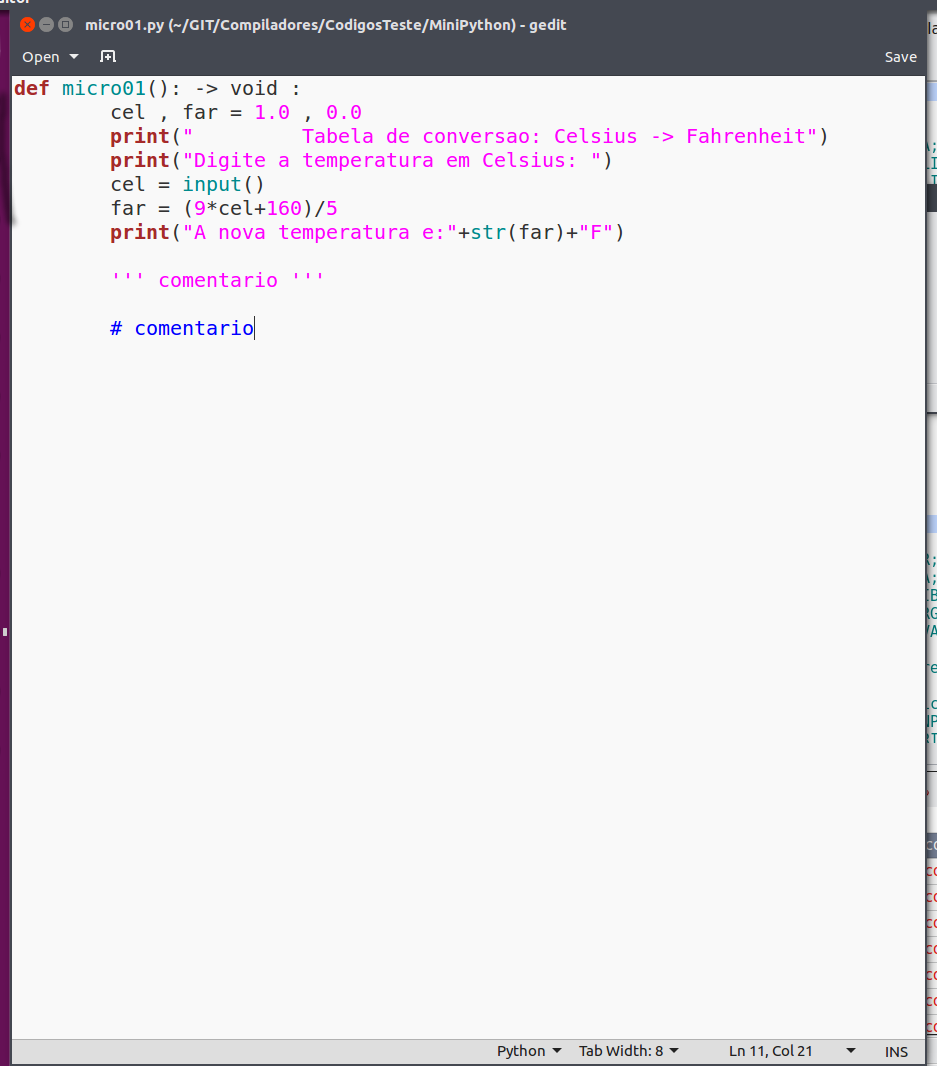
\includegraphics[scale=0.5]{Figures/comentario}
	\end{figure}
	
	\newpage
	A saída não considerou os comentários:
	
	\begin{lstlisting}[caption=Analisador Léxico com Comentário]
	- : tokens =
	[Lexico.DEF; Lexico.ID "micro01"; Lexico.APAR; Lexico.FPAR; Lexico.DPONTOS;
	Lexico.SETA; Lexico.VOID; Lexico.DPONTOS; Lexico.NOVALINHA; Lexico.INDENTA;
	Lexico.ID "cel"; Lexico.VIRG; Lexico.ID "far"; Lexico.ATRIB;
	Lexico.LITINT 1; Lexico.PONTO; Lexico.LITINT 0; Lexico.VIRG;
	Lexico.LITINT 0; Lexico.PONTO; Lexico.LITINT 0; Lexico.NOVALINHA;
	Lexico.PRINT; Lexico.APAR;
	Lexico.LITSTRING "\t\tTabela de conversao: Celsius -> Fahrenheit";
	Lexico.FPAR; Lexico.NOVALINHA; Lexico.PRINT; Lexico.APAR;
	Lexico.LITSTRING "Digite a temperatura em Celsius: "; Lexico.FPAR;
	Lexico.NOVALINHA; Lexico.ID "cel"; Lexico.ATRIB; Lexico.INPUT; Lexico.APAR;
	Lexico.FPAR; Lexico.NOVALINHA; Lexico.ID "far"; Lexico.ATRIB; Lexico.APAR;
	Lexico.LITINT 9; Lexico.VEZES; Lexico.ID "cel"; Lexico.MAIS;
	Lexico.LITINT 160; Lexico.FPAR; Lexico.DIVIDIDO; Lexico.LITINT 5;
	Lexico.NOVALINHA; Lexico.PRINT; Lexico.APAR;
	Lexico.LITSTRING "A nova temperatura e:"; Lexico.MAIS; Lexico.STR;
	Lexico.APAR; Lexico.ID "far"; Lexico.FPAR; Lexico.MAIS;
	Lexico.LITSTRING "F"; Lexico.FPAR; Lexico.NOVALINHA; Lexico.NOVALINHA;
	Lexico.DEDENTA; Lexico.EOF]
	\end{lstlisting}
	
\section{Analisador Sintático}

\subsection{Teste de Gramática}

	Foi implementado, o algoritmo da seguinte gramática em virtude de aprofundar os conhecimentos do processo de análise sintática.
	
	\begin{figure}[h!]
		\centering
		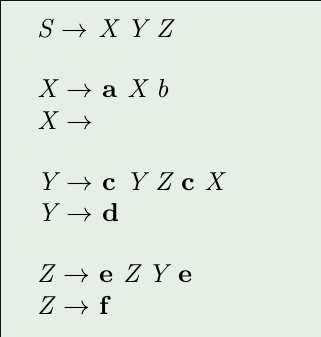
\includegraphics[scale=0.5]{Figures/gramatica.png}
	\end{figure}	
	
	\newpage
	É importante ressaltar os conceitos de first e follow. First é o conjunto de símbolos que ocorrem no início de uma determinada regra  e follow é o que pode aparecer depois da ocorrência de um determinado símbolo.
	
	Facilita o entendimento do código quando é feita a tabela de first e follow e também a tabela com as regras de derivação. Nesse caso, as tabelas foram retiradas dos slides da aula.
	
	\begin{figure}[h!]
		\centering
		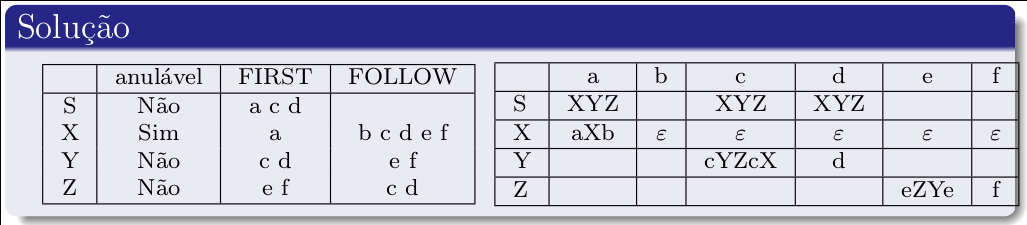
\includegraphics[scale=0.5]{Figures/tabela-gramatica.png}
	\end{figure}
	
	Segue a sequencia de passos para compilar e rodar os programas:
	
	\begin{lstlisting}[caption=Analisador Léxico com Comentário]
	ocamllex lexico.mll
	ocamlc -c sintatico.mli
	ocamlc -c lexico.ml
	
	rlwrap ocaml
	load "lexico.cmo";;
	"sintaticoArv.ml";;
	teste();;
	\end{lstlisting}
	
	
	Seguem os testes referentes a esse processo.
	
	\textbf{Entrada:} abdf
	
	\begin{figure}[h!]
		\centering
		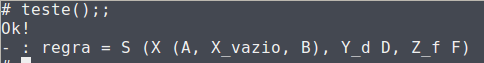
\includegraphics[scale=0.7]{Figures/testeg1.png}
	\end{figure}
	
	\textbf{Entrada:} cdfcf
	
	\begin{figure}[h!]
		\centering
		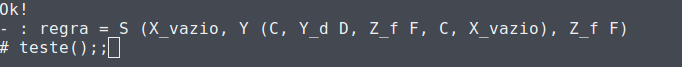
\includegraphics[scale=0.7]{Figures/testeg2.png}
	\end{figure}
	
	Para uma entrada equivocada, o código gera um erro:
	
	\textbf{Entrada:} bcdac
	\begin{figure}[h!]
		\centering
		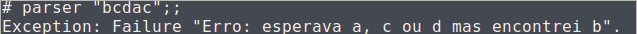
\includegraphics[scale=0.7]{Figures/testeg3.png}
	\end{figure}
	
	\subsection{Códigos Fonte}
	
	Seguem os códigos fonte referentes a implementação do programa:
	
	\begin{lstlisting}[caption=léxico.mll, language=python]
	{
	open Lexing
	open Printf
	open Sintatico
	
	
	let incr_num_linha lexbuf = 
	let pos = lexbuf.lex_curr_p in
	lexbuf.lex_curr_p <- { pos with
	pos_lnum = pos.pos_lnum + 1;
	pos_bol = pos.pos_cnum;
	}
	
	let msg_erro lexbuf c =
	let pos = lexbuf.lex_curr_p in
	let lin = pos.pos_lnum
	and col = pos.pos_cnum - pos.pos_bol - 1 in
	sprintf "%d-%d: caracter desconhecido %c" lin col c
	
	
	}
	
	rule token = parse 
	| 'a'        {A}
	| 'b'        {B}
	| 'c'        {C}
	| 'd'        {D}
	| 'e'        {E}
	| 'f'        {F}
	| _ as c  { failwith (msg_erro lexbuf c) }
	| eof        { EOF }
	
	
	
	
	\end{lstlisting}
	
	
	\begin{lstlisting}[caption=sintatico.mli, language=python]
	type tokens = A 
	| B
	| C
	| D
	| E
	| F
	| EOF
	
	\end{lstlisting}
	
	
	\begin{lstlisting}[caption=sintaticoArv.ml, language=python]
	(* Parser preditivo *)
	load "lexico.cmo";;
	open Sintatico;;
	
	type rule = S of rule * rule * rule
	| X of tokens * rule * tokens
	| Y of tokens * rule * rule * tokens * rule
	| Z of tokens * rule * rule * tokens
	| X_empty
	| Y_d of tokens
	| Z_f of tokens
	
	let tk = ref EOF (* variavel global para o token atual *)
	let lexbuf = ref (Lexing.from_string "")
	
	(* le o proximo token *)             
	let prox () = tk := Lexico.token !lexbuf
	
	let to_str tk =
	match tk with
	A -> "a"
	| B -> "b"
	| C -> "c"
	| D -> "d"
	| E -> "e"
	| F -> "f"
	| EOF -> "eof"
	
	let erro esp =
	let msg = Printf.sprintf "Erro: esperava %s mas encontrei %s"
	esp (to_str !tk)
	in
	failwith msg
	
	let consome t = if (!tk == t) then prox() else erro (to_str t)
	
	let rec ntS () =
	match !tk with
	A    
	|C     
	|D     -> 
	let cmd1 = ntX() in
	let cmd2 = ntY() in
	let cmd3 = ntZ() in
	S (cmd1, cmd2, cmd3)
	| _ -> erro "a, c ou d"
	and ntX () =
	match !tk with
	B
	|C
	|D
	|E
	|F    -> X_empty
	|A    -> let _ = consome A in 
	let cmd = ntX() in
	let _ = consome B in
	X (A, cmd, B)
	| _ -> erro "a"                               
	and ntY () =
	match !tk with
	C    -> let _ = consome C in
	let cmd = ntY() in
	let cmd2 = ntZ() in
	let _ = consome C in
	let cmd3 = ntX() in
	Y (C,cmd,cmd2, C, cmd3)
	|D     -> let _ = consome D in
	Y_d (D)
	|_     -> erro "c ou d"
	and ntZ () = 
	match !tk with
	E    -> let _ = consome E in
	let cmd = ntZ() in
	let cmd2 = ntY() in
	let _ = consome E in
	Z (E, cmd, cmd2, E)
	|F    -> let _ = consome F in
	Z_f (F)
	|_    -> erro "e ou f"                                           
	
	let parser str =
	lexbuf := Lexing.from_string str;
	prox (); (* inicializa o token *)
	let arv = ntS () in
	match !tk with
	EOF -> let _ = Printf.printf "Ok!\n" in arv
	| _ -> erro "fim da entrada"
	
	let teste str =
	let entrada = str
	in
	parser entrada
	
	\end{lstlisting}
	

\section{Sintático Usando Menhir}

Para usar o Menhir foi necessário instalar o opam (gerenciador de dependências do Ocaml)

	\noindent\fbox{%
		\parbox{\textwidth}{%
			$>$ sudo apt-get install opam m4
			
			$>$	opam init
			
			$>$ eval 'opam config env'
			
			$>$ opam install menhir
		}%
	}


Para otimizar o processo de compilação, foi utilizado o arquivo .ocamlinit

\noindent\fbox{%
	\parbox{\textwidth}{%
		$\sharp$ directory "\_build";;
		
		$\sharp$ load "lexico.cmo";;
		
		$\sharp$ load "parser.cmo";;
		
		$\sharp$ "pre\_processador.cmo";;
		
		$\sharp$ "main.cmo";;
		
		$\sharp$ open Main;;
		
		$\sharp$ open Ast;;
		
		
	}%
}

O processo para a compilação é:
\textbf{ocamlbuild -use-menhir main.byte}


\subsection{Testes}

Foram testados os seguintes problemas.
Seguem as saídas:

	\begin{lstlisting}[caption=sintatico.mli, language=python]
	def micro11() -> int:
		numero = 0
		x =0
		print("numero")
		numero = input()
		numero = verifica(numero)
		if x ==1:
			print("Positivo")
		if x ==0:
			print("zero")
		else:
			print("Negativo")
	
		return 0
	
	
	def verifica(n:int) -> int:
		res = 0
		if n>0:
			res = 1
		if n<0:
			res = 2
		else:
			res = 0
		
		return res
	
	micro11()
	
	\end{lstlisting}
	
	\textbf{{\large Saída}}
	
	\begin{figure}[!h]
		\centering
		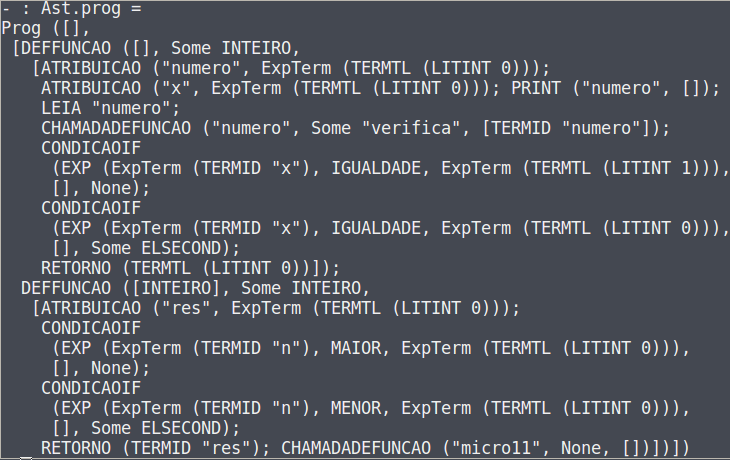
\includegraphics[scale=0.5]{Figures/menhir0}
	\end{figure}
	
	
	\begin{lstlisting}[caption=sintatico.mli, language=python]
	import x
	def micro(): 
		numero =0
		numero = input()
		if numero>= 100:
			if numero<= 200:
				print("e")
			else:
				print("d")
		else:
			print("f")
	
		micro()
	
	\end{lstlisting}
	
	\textbf{{\large Saída}}
	
	\begin{figure}[!h]
		\centering
		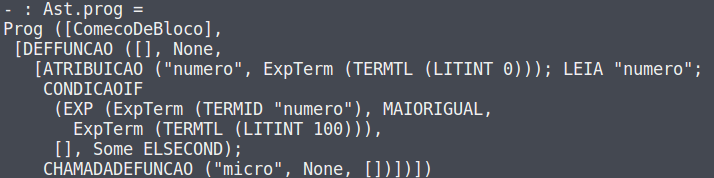
\includegraphics[scale=0.5]{Figures/menhir1}
	\end{figure}
\newpage	
	\begin{lstlisting}[caption=sintatico.mli, language=python]
	def nano():
		n=1
		m=2
		x=5
		while x >n:
			n = 4 + m
			print("n",n)
	
	
	\end{lstlisting}
	
	\textbf{{\large Saída}}
	
	\begin{figure}[!h]
		\centering
		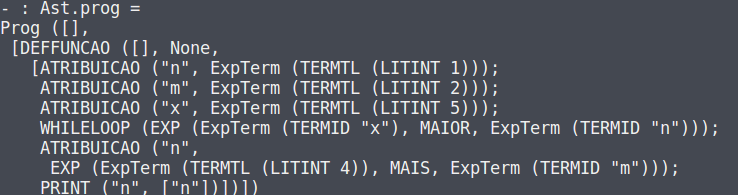
\includegraphics[scale=0.5]{Figures/menhir2}
	\end{figure}
	\newpage
	
	\begin{lstlisting}[caption=sintatico.mli, language=python]
	def micro08():
		numero =1
		while numero < 0 or numero >0:
			print("digite")
			numero = input()
			if numero > 10:
				print("maior10")
			else:
				print("menor10")
		
		
		micro08()
	
	\end{lstlisting}
	
	\textbf{{\large Saída}}
	
	\begin{figure}[!h]
		\centering
		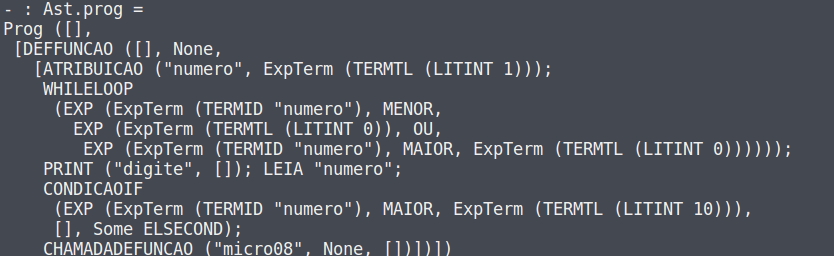
\includegraphics[scale=0.5]{Figures/menhir3}
	\end{figure}
	
	\begin{lstlisting}[caption=sintatico.mli, language=python]
	def micro06() -> int:
		numero = 0
		
		print("Digite um numero de 1 a 5: ")
		numero = input()
		if numero ==1: 
			print("Um")
		elif numero == 2:
			print("Dois")
		elif numero ==3:
			print("Tres")
		elif numero ==4:
			print("Quatro")
		elif numero ==5:
			print("Cinco")
		else:
			print("Numero Invalido!!!")
		
		micro06()
	
	\end{lstlisting}
	
	\textbf{{\large Saída}}
	
	\begin{figure}[!h]
		\centering
		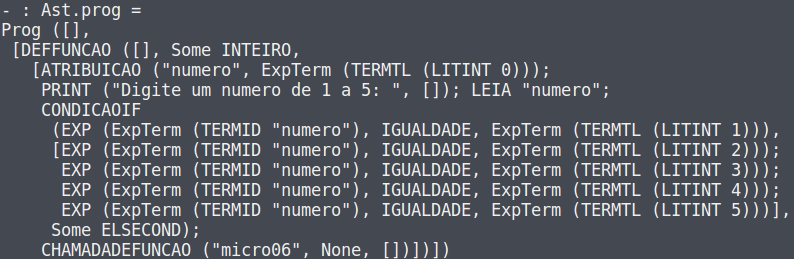
\includegraphics[scale=0.5]{Figures/menhir4}
	\end{figure}

	
	\section{Analisador Semântico}
	
	Em virtude de incorporar o analisador semântico ao trabalho ja feito, foram realizadas mudanças nos arquivos do sintático e léxico a fim de facilitar a integração.
	
	Agora, as variáveis do código estão sendo exibidas com os parâmetros linha e coluna. Segue um exemplo:
	
	
		\begin{lstlisting}[caption=sintatico.mli, language=python]

		def funcaozona() -> int:
	
			inputf(valor)
		
			x = valor + 1.0
			
			return 1
	
	
	
	\end{lstlisting}
	
	\newpage
	\textbf{{\large Saída}}
	
	\begin{figure}[!h]
		\centering
		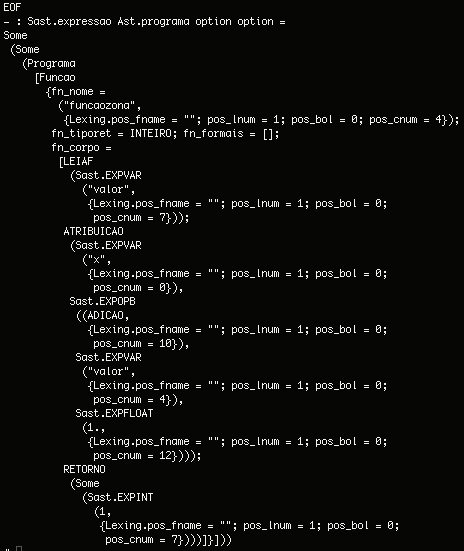
\includegraphics[scale=0.5]{Figures/sintaticoNovo}
	\end{figure}
	
	\subsection{Testes}
	
	Seguem os testes que tem como saída a árvores semântica tipada. Para aumentar o controle de tipos, o comando input foi alterado em tres outros comandos, inputi, inputs e inputf que representam leitura de tipos inteiro, string e real.
	
			\begin{lstlisting}[caption=sintatico.mli, language=python]
	
def micro11() -> int:
	numero = 0
	x =0
	print("numero")
	inputs(numero)
	numero = verifica(numero)
	if x ==1:
		print("Positivo")
	if x ==0:
		print("zero")
	else:
		print("Negativo")
	
	return 0


def verifica(n:int) -> int:
	res = 0
	if n>0:
		res = 1
	if n<0:
		res = 2
	else:
		res = 0
	
	return res
	
	x  = 2

	
	
	
	\end{lstlisting}
	
	
	\textbf{{\large Saída}}
	
	\begin{figure}[!h]
		\centering
		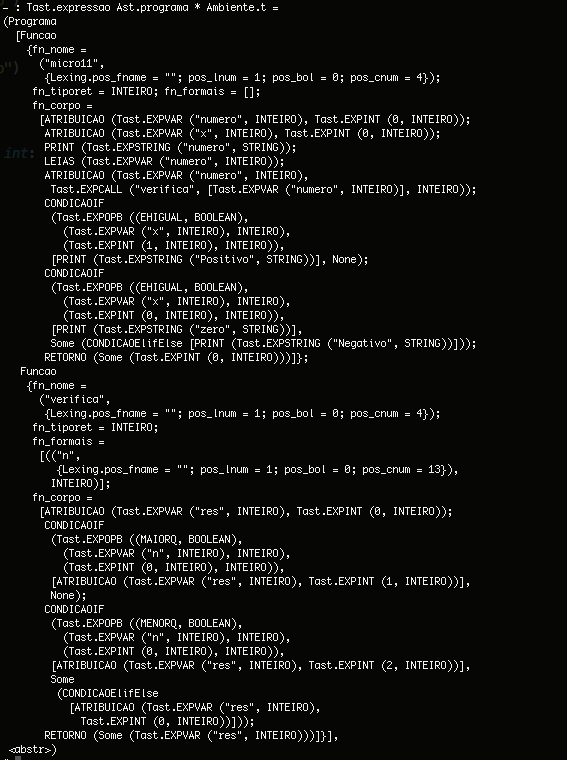
\includegraphics[scale=0.5]{Figures/e1semantico}
	\end{figure}
	
	\newpage
\begin{lstlisting}[caption=sintatico.mli, language=python]
def micro() -> None: 
	numero =0
	inputi()
	if numero>= 100:
		if numero<= 200:
			print("e")
		else:
			print("d")
	else:
		print("f")

micro()

\end{lstlisting}


\textbf{{\large Saída}}

\begin{figure}[!h]
	\centering
	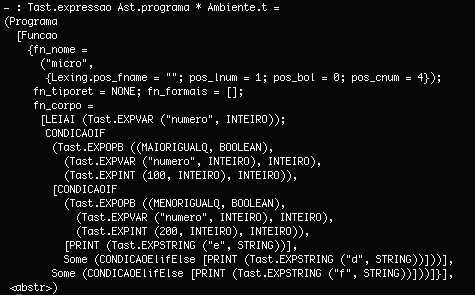
\includegraphics[scale=0.5]{Figures/e2semantico}
\end{figure}

\begin{lstlisting}[caption=sintatico.mli, language=python]

def nano() -> None:
	n=1
	m=2
	x=5
	while x >n:
		n = 4 + m
		print("n",n)


\end{lstlisting}


\textbf{{\large Saída}}

\begin{figure}[!h]
	\centering
	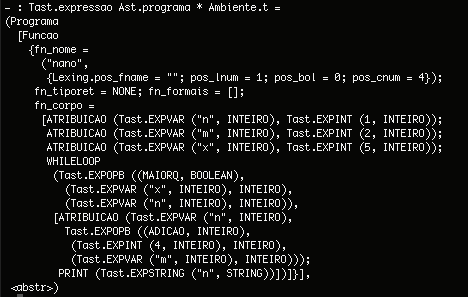
\includegraphics[scale=0.5]{Figures/e3semantico}
\end{figure}

\newpage
\begin{lstlisting}[caption=sintatico.mli, language=python]

def micro08() -> None:
	numero =1
	while numero < 0 or numero >0:
		print("digite")
		inputi(numero)
		if numero > 10:
			print("maior10")
		else:
			print("menor10")
	

micro08()

\end{lstlisting}


\textbf{{\large Saída}}

\begin{figure}[!h]
	\centering
	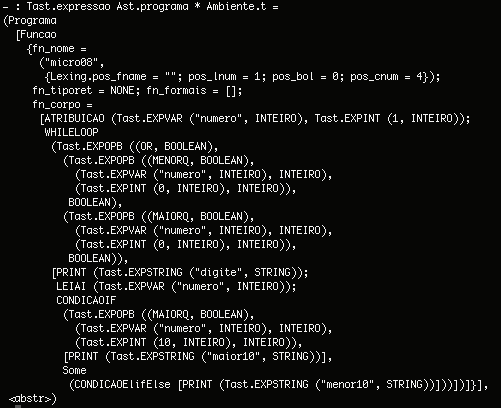
\includegraphics[scale=0.5]{Figures/e4semantico}
\end{figure}

\newpage
\begin{lstlisting}[caption=sintatico.mli, language=python]

def micro06() -> int:
	numero = 0
	
	print("Digite um numero de 1 a 5: ")
	inputi(numero)
	if numero ==1: 
		print("Um")
	elif numero == 2:
		print("Dois")
	elif numero ==3:
		print("Tres")
	elif numero ==4:
		print("Quatro")
	elif numero ==5:
		print("Cinco")
	else:
		print("Numero Invalido!!!")

micro06()

\end{lstlisting}


\textbf{{\large Saída}}

\begin{figure}[!h]
	\centering
	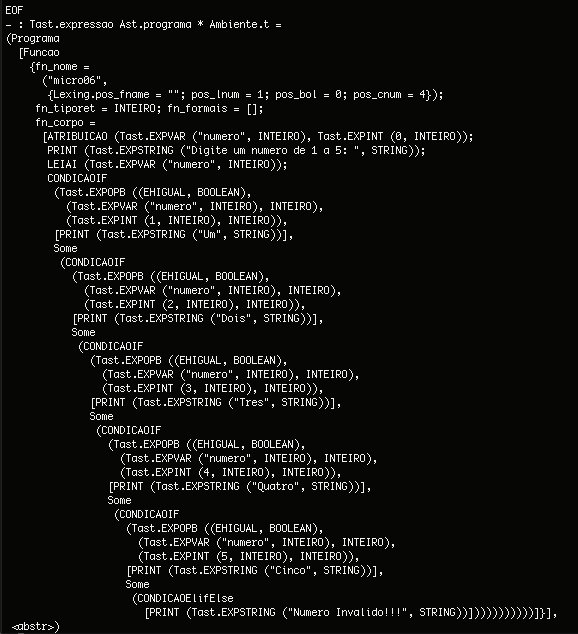
\includegraphics[scale=0.5]{Figures/e6semantico}
\end{figure}


\begin{lstlisting}[caption=sintatico.mli, language=python]

def micro10() -> None:
	numero =0
	fat = 0
	print("Digite um numero: ")
	inputi(numero)
	fat = fatorial(numero)
	
	print("O fatorial eh ",fat)

def fatorial(n: int) -> int:
	if n <=0:
		return 1
	else:
		return n * fatorial(n - 1)

micro10( )

\end{lstlisting}

\textbf{{\large Saída}}

\begin{figure}[!h]
	\centering
	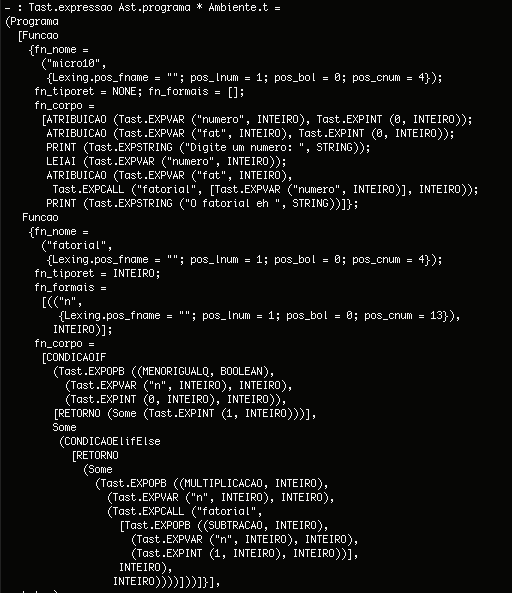
\includegraphics[scale=0.5]{Figures/e7semantico}
\end{figure}



\subsection{Testes Com Erros}


Seguem os testes em que o código foi deixado propositalmente com erros semânticos.


\begin{lstlisting}[caption=sintatico.mli, language=python]

def func() -> int:

	inputf(valor)
	
	x = valor + 1.0
	
	return "uma string que nao deveria estar aqui"

\end{lstlisting}


\textbf{{\large Saída}}

\begin{figure}[!h]
	\centering
	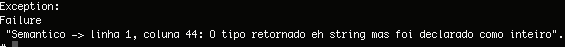
\includegraphics[scale=0.5]{Figures/erro1semantico}
\end{figure}	
	
	
	
\begin{lstlisting}[caption=sintatico.mli, language=python]

def func() -> int:

	inputf(valor)

	x = valor + 1.0

	return "uma string que nao deveria estar aqui"

\end{lstlisting}


\textbf{{\large Saída}}

\begin{figure}[!h]
	\centering
	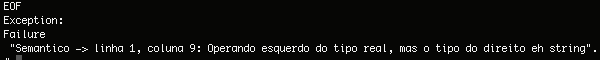
\includegraphics[scale=0.5]{Figures/erro2semantico}
\end{figure}	


\newpage
\section{Interpretador Usando Menhir}


\subsection{Execução}

Para executar o interpretador deve-se digitar

\textbf{ ocamlbuild -use-ocamlfind -use-menhir -menhir "menhir --table" -package menhirLib interpreteTeste.byte
	}
	
E depois entrar no ocaml usando \textbf{rlwrap ocaml}. Após isso,  o interpretador pode ser executado com \textbf{$\sharp$ interprete "../testes/nomeDoArquivo.py"}.

\textbf{OBS.:} deve-se, antes disso, excluir o diretorio build com \textbf{rm -rf \_build} e excluir o arquivo interpretadorTeste.byte caso ele existe com \textbf{rm interpretadorTeste.byte}.

\newpage

\subsection{Testes}
O interpretador consiste em executar o código usando as partes léxica, sintatica e semântica feitas durante o semestre. Seguem os testes



\begin{lstlisting}[caption=sintatico.mli, language=python]
def main() -> int:
	numero = 0
	x =0
	print("Digite um numero: ")
	inputi(numero)
	numero = verifica(numero)
	
	if numero == 1:
		print("Positivo")
	elif numero == 0:
		print("zero")
	else:
		print("Negativo")

	return 0


def verifica(n:int) -> int:
	res = 0
	if n > 0:
		return 1
	if n < 0:
		return 3
	else:
		return 0

main()

\end{lstlisting}


\textbf{{\large Saída}}

\begin{figure}[!h]
	\centering
	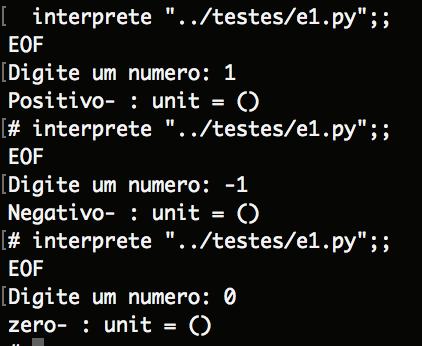
\includegraphics[scale=0.8]{Figures/inter1}
\end{figure}	

\newpage
	
\begin{lstlisting}[caption=sintatico.mli, language=python]
def main() -> None: 
	print("Digite um numero:  ")
	inputi(numero)
	if numero>= 100:
		if numero<= 200:
			print("\n numero entre 100 e 200")
		else:
			print("\nnumero maior que 200")
	else:
		print("\nnumero menor que 100")


main()
\end{lstlisting}

\newpage
\textbf{{\large Saída}}

\begin{figure}[!h]
	\centering
	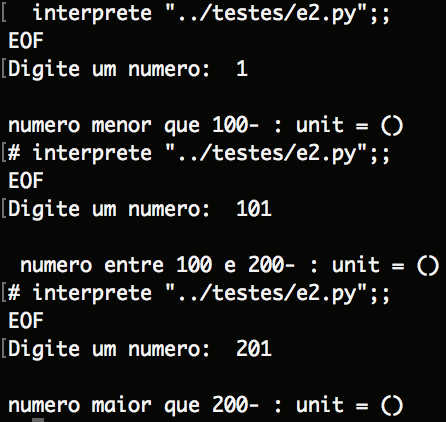
\includegraphics[scale=0.8]{Figures/inter2}
\end{figure}	

\begin{lstlisting}[caption=sintatico.mli, language=python]
def main() -> None:
	n=1
	m=2
	x=50
	while n < x:
		n = n + 4 + m
		print("n = ")
		print(n)
		print("\n")

main()
\end{lstlisting}

\newpage
\textbf{{\large Saída}}

\begin{figure}[!h]
	\centering
	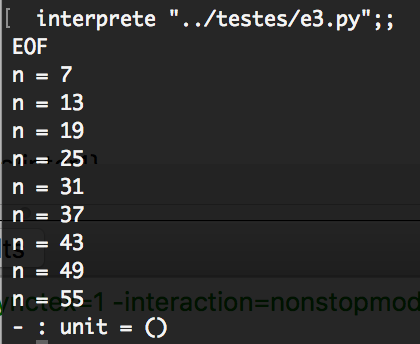
\includegraphics[scale=0.8]{Figures/inter3}
\end{figure}	

\begin{lstlisting}[caption=sintatico.mli, language=python]
def main() -> None:
	numero =1
	while numero < 0 or numero >0:
		print("\n Digite um numero: ")
		inputi(numero)
		if numero > 10:
			print("\n Numero maior que 10")
		else:
			print("\n Numero menor que 10")


main()
\end{lstlisting}

\newpage
\textbf{{\large Saída}}

\begin{figure}[!h]
	\centering
	\includegraphics[scale=0.8]{Figures/inter4}
\end{figure}	

\begin{lstlisting}[caption=sintatico.mli, language=python]
def main() -> int:
	numero = 0
	
	print("Digite um numero de 1 a 5: ")
	inputi(numero)
	if numero ==1: 
		print("Um")
	elif numero == 2:
		print("Dois")
	elif numero ==3:
		print("Tres")
	elif numero ==4:
		print("Quatro")
	elif numero ==5:
		print("Cinco")
	else:
		print("Numero Invalido!!!")

main()
\end{lstlisting}

\newpage
\textbf{{\large Saída}}

\begin{figure}[!h]
	\centering
	\includegraphics[scale=0.8]{Figures/inter6}
\end{figure}	

\begin{lstlisting}[caption=sintatico.mli, language=python]
def main() -> None:
	numero =0
	fat = 0
	print("Digite um numero: ")
	inputi(numero)
	fat = fatorial(numero)
	
	print("O fatorial eh ")
	print(fat)

def fatorial(n: int) -> int:
	if n <= 0:
		return 1
	else:
		return n * fatorial(n - 1)

main()
\end{lstlisting}

\newpage
\textbf{{\large Saída}}

\begin{figure}[!h]
	\centering
	\includegraphics[scale=0.8]{Figures/inter7}
\end{figure}	


\begin{lstlisting}[caption=sintatico.mli, language=python]
def main() -> None:
	print("Digite um numero: ")
	inputi(i)
	while i < 10:
		print(i)
		print(" ")
		i = i +1

\end{lstlisting}


\textbf{{\large Saída}}

\begin{figure}[!h]
	\centering
	\includegraphics[scale=0.8]{Figures/interex1}
\end{figure}	
	


\begin{lstlisting}[caption=sintatico.mli, language=python]

def fib(n:int) -> int:
	if n <= 1:
		return 1
	else:
		return fib( n - 1 ) + fib( n - 2 )

def fat(n:int) -> int:
	if n <= 1:
		return 1
	else:
		return n * fat( n - 1)


def main() -> None:
	op = 1
	while op != 0:
		print("| 1 - fib\n| 2 - fat\n| 0 - sair\n-> ")
		inputi(op)
		if op == 1:
			print("Digite um numero para calcular o fibonacci: ")
			inputi(f)
			print(" fibonacci :")
			print(fib(f))
		elif op == 2:
			print("Digite um numero para calcular o fatorial: ")
			inputi(f)
			print(" fatorial :")
			print(fat(f))
		else:
			op =0
			print("\n")
			
			
main()
\end{lstlisting}


\textbf{{\large Saída}}

\begin{figure}[!h]
	\centering
	\includegraphics[scale=0.8]{Figures/interex4}
\end{figure}	

\section{Erros gerados pelo interpretador}

Nesta seção, serão exibidos os erros gerados pelo interpretador dado como entrada códigos em python propositalmente errados.

\vspace{0.5cm}
\textbf{\huge Erro Semântico}

\begin{lstlisting}[caption=sintatico.mli, language=python]
def main() -> str:
	n=1
	m=2
	x=50
	while n < x:
		n = n + 4 + m
		print("n = ")
		print(n)
		print("\n")

	return 1

main()
\end{lstlisting}


\textbf{{\large Saída}}

\begin{figure}[!h]
	\centering
	\includegraphics[scale=0.8]{Figures/intererro1}
\end{figure}

\vspace{0.5cm}
\textbf{\huge Erro Sintático}

\begin{lstlisting}[caption=sintatico.mli, language=python]

def main() -> None:
	n=1
	m=2
	x=50
	while n < x:
		n = n + 4 + m
		print("n = "
		print(n)
		print("\n")

main()

\end{lstlisting}


\textbf{{\large Saída}}

\begin{figure}[!h]
	\centering
	\includegraphics[scale=0.8]{Figures/intererro2}
\end{figure}


\vspace{0.5cm}
\textbf{\huge Erro Léxico}
	
\begin{lstlisting}[caption=sintatico.mli, language=python]
def main() -> None:
	n=1
	@=2
	x=50
	while n < x:
		n = n + 4 + m
		print("n = ")
		print(n)
		print("\n")

main()
\end{lstlisting}


\textbf{{\large Saída}}

\begin{figure}[!h]
	\centering
	\includegraphics[scale=0.8]{Figures/intererro3}
\end{figure}
	
	
	
\renewcommand{\appendixtocname}{Ap\^endice}
\renewcommand{\appendixpagename}{Ap\^endice}
\begin{appendices}
	
	\chapter{lexico.mll}
		
	\begin{lstlisting}[caption=lexico.mll, language=python]
	
	{
	open Sintatico
	open Lexing
	open Printf
	
	exception Erro of string
	
	let booleano nbool = 
	match nbool with
	| "True" -> 1
	| "False" -> 0
	| _ -> failwith "Erro: nao eh valor booleano"  
	
	let nivel_par = ref 0
	
	let incr_num_linha lexbuf =
	let pos = lexbuf.lex_curr_p in
	lexbuf.lex_curr_p <- { pos with
	pos_lnum = pos.pos_lnum + 1;
	pos_bol = pos.pos_cnum;
	}
	
	let msg_erro lexbuf c =
	let pos = lexbuf.lex_curr_p in
	let lin = pos.pos_lnum
	and col = pos.pos_cnum - pos.pos_bol - 1 in
	sprintf "%d-%d: caracter desconhecido %c" lin col c
	
	let erro lin col msg =
	let mensagem = sprintf "%d-%d: %s" lin col msg in
	failwith mensagem
	
	let pos_atual lexbuf = lexbuf.lex_start_p
	
	}
	
	let digito = ['0' - '9']
	let int = '-'? * digito+
	let float = '-'? * digito+ * '.' * digito+
	let comentario = "#"[ ^ '\n' ]*
	let linha_em_branco = [' ' '\t' ]* comentario
	let restante = [^ ' ' '\t' '\n' ] [^ '\n']+
	let brancos = [' ' '\t']+
	let novalinha = '\r' | '\n' | "\r\n"
	let letra = [ 'a'-'z' 'A' - 'Z']
	let identificador = letra ( letra | digito | '_' )*
	
	(* O pre processador necessario para contabilizar a identacao *)
	rule preprocessador indentacao = parse
	linha_em_branco         { preprocessador 0 lexbuf } (* ignora brancos *)
	| [' ' '\t' ]+ '\n'       { incr_num_linha lexbuf;
	preprocessador 0 lexbuf } (* ignora brancos *)
	| ' '                     { preprocessador (indentacao + 1) lexbuf }
	| '\t'                    { let nova_ind = indentacao + 8 - (indentacao mod 8) 
	in preprocessador nova_ind lexbuf }
	| novalinha               { incr_num_linha lexbuf;
	preprocessador 0 lexbuf }
	| restante as linha {
	let rec tokenize lexbuf =
	let tok = token lexbuf in
	match tok with
	EOF -> []
	| _ -> tok :: tokenize lexbuf in
	let toks = tokenize (Lexing.from_string linha) in
	Linha(indentacao,!nivel_par, toks)
	}
	| eof { nivel_par := 0; EOF }
	
	(* O analisador lexico a ser chamado apos o pre processador *)
	and token = parse
	brancos            { token lexbuf }
	| comentario         { token lexbuf }
	| "'''"              { comentario_bloco 0 lexbuf; }
	| ">="               { MAIORIGUAL (pos_atual lexbuf)}
	| "<="               { MENORIGUAL (pos_atual lexbuf)}
	| "->"               { SETA (pos_atual lexbuf)}
	| "=="               { IGUALDADE (pos_atual lexbuf)}
	| "!="               { DIFERENTE (pos_atual lexbuf)}
	| '('                { incr(nivel_par); APAR(pos_atual lexbuf)}
	| ')'                { decr(nivel_par); FPAR(pos_atual lexbuf)}
	| ','                { VIRG (pos_atual lexbuf)}
	| '+'                { MAIS  (pos_atual lexbuf)}
	| '-'                { MENOS (pos_atual lexbuf) }
	| '*'                { VEZES  (pos_atual lexbuf)}
	| '/'                { DIVIDIDO (pos_atual lexbuf)}
	| '='                { ATRIB (pos_atual lexbuf)}
	| ':'                { DPONTOS (pos_atual lexbuf)}
	| '<'                { MENOR (pos_atual lexbuf)}
	| '>'                { MAIOR (pos_atual lexbuf)}
	| '%'		             { MODULO (pos_atual lexbuf)}
	| "or"               { OU (pos_atual lexbuf)}
	| "if"               { IF (pos_atual lexbuf)}
	| "else"             { ELSE (pos_atual lexbuf)}
	| "while"            { WHILE (pos_atual lexbuf)}
	| "for"              { FOR (pos_atual lexbuf)}
	| "return"           { RETURN (pos_atual lexbuf)}
	| "def"              { DEF (pos_atual lexbuf)}
	| "int"              { INT (pos_atual lexbuf)}
	| "float"            { FLOAT (pos_atual lexbuf)}
	| "bool"             { BOOL (pos_atual lexbuf)}
	| "and"              { E   (pos_atual lexbuf) }
	| "in"               { IN (pos_atual lexbuf)}
	| "range"            { RANGE (pos_atual lexbuf)}
	| "None"             { NONE (pos_atual lexbuf)}
	| "elif"	           { ELIF (pos_atual lexbuf)}
	| "print"            { PRINT (pos_atual lexbuf)}
	| "str"              { STR (pos_atual lexbuf)}
	| "inputi"            { INPUTI (pos_atual lexbuf)}
	| "inputf"            { INPUTF (pos_atual lexbuf)}
	| "inputs"            { INPUTS (pos_atual lexbuf)}
	| "not"		           { NOT (pos_atual lexbuf)}
	| "True"             { LITBOOL(true,pos_atual lexbuf)}
	| "False"            { LITBOOL(false,pos_atual lexbuf)}
	| int as num         { LITINT (int_of_string num, pos_atual lexbuf) } 
	| float as num       { LITFLOAT (float_of_string num, pos_atual lexbuf) }
	| digito+ as numint  {let num = int_of_string numint in LITINT (num, pos_atual lexbuf)}
	| identificador as id { ID (id, pos_atual lexbuf) }
	| '"'        { let pos = lexbuf.lex_curr_p in
	let lin = pos.pos_lnum
	and col = pos.pos_cnum - pos.pos_bol - 1 in
	let buffer = Buffer.create 1 in 
	let str = leia_string lin col buffer lexbuf in
	LITSTRING (str, pos_atual lexbuf) }
	| _ as c  { failwith (msg_erro lexbuf c) }
	| eof        { EOF }
	
	and comentario_bloco n = parse
	"'''"      { if n=0 then token lexbuf 
	else comentario_bloco (n-1) lexbuf }
	| "'''"       { comentario_bloco (n+1) lexbuf }
	| novalinha  { incr_num_linha lexbuf; comentario_bloco n lexbuf }
	| _          { comentario_bloco n lexbuf }
	| eof     { raise (Erro "Comentario nao terminado") }
	
	and leia_string lin col buffer = parse
	'"'     { Buffer.contents buffer}
	| "\\t"    { Buffer.add_char buffer '\t'; leia_string lin col buffer lexbuf }
	| "\\n"    { Buffer.add_char buffer '\n'; leia_string lin col buffer lexbuf }
	| '\\' '"'  { Buffer.add_char buffer '"'; leia_string lin col buffer lexbuf }
	| '\\' '\\' { Buffer.add_char buffer '\\'; leia_string lin col buffer lexbuf }
	| _ as c    { Buffer.add_char buffer c; leia_string lin col buffer lexbuf }
	| eof      { erro lin col "A string nao foi fechada"}
	
	
	
	
	
	
	\end{lstlisting}
	
	\newpage
	\chapter{semantico.mll}
	
	\begin{lstlisting}[caption=semantico.mll, language=python]
	
	module Amb = Ambiente
	module A = Ast
	module S = Sast
	module T = Tast
	
	let rec posicao exp = 
	let open S in
	match exp with 
	| EXPVAR       (_,pos)      -> pos
	| EXPINT       (_,pos)      -> pos
	| EXPSTRING    (_,pos)      -> pos
	| EXPBOOL      (_,pos)      -> pos
	| EXPFLOAT     (_,pos)      -> pos
	| EXPOPB    ((_,pos),_,_) -> pos
	| EXPOPU    ((_,pos),_)   -> pos
	| EXPCALL     ((_,pos),_)   -> pos
	
	
	type classe_op = Aritmetico | Relacional | Logico
	
	let classifica op =
	let open A in
	match op with
	ADICAO
	| SUBTRACAO
	| MULTIPLICACAO
	| DIVISAO
	| MOD       -> Aritmetico
	| MAIORQ
	| MENORQ
	| MAIORIGUALQ
	| MENORIGUALQ
	| EHIGUAL
	| EHDIFERENTE   -> Relacional
	| AND
	| NEGACAO
	| OR  -> Logico
	
	let msg_erro_pos pos msg =
	let open Lexing in
	let lin = pos.pos_lnum
	and col = pos.pos_cnum - pos.pos_bol - 1 in
	Printf.sprintf "Semantico -> linha %d, coluna %d: %s" lin col msg
	
	(*  argumento nome e do tipo S.tipo  *)
	let msg_erro nome msg =
	let pos = snd nome in 
	msg_erro_pos pos msg
	
	let nome_tipo t =
	let open A in
	match t with
	INTEIRO     -> "inteiro"
	| STRING     -> "string"
	| BOOLEAN    -> "booleano"
	| REAL   -> "real"
	| NONE    -> "vazio"
	
	let mesmo_tipo pos msg tinf tdec =
	if tinf <> tdec then
	let msg = Printf.sprintf msg (nome_tipo tinf) (nome_tipo tdec) in
	failwith (msg_erro_pos pos msg)
	
	let rec infere_exp amb exp =
	match exp with
	
	| S.EXPINT   i -> (T.EXPINT   (fst i, A.INTEIRO  ), A.INTEIRO  )
	| S.EXPSTRING   s -> (T.EXPSTRING   (fst s, A.STRING  ), A.STRING  )
	| S.EXPBOOL  b -> (T.EXPBOOL  (fst b, A.BOOLEAN ), A.BOOLEAN )
	| S.EXPFLOAT f -> (T.EXPFLOAT (fst f, A.REAL), A.REAL)
	| S.EXPVAR variavel ->
	let nome = fst variavel in
	(try begin
	(match (Amb.busca amb nome) with
	| Amb.EntVar tipo -> (T.EXPVAR (nome, tipo), tipo)
	| Amb.EntFun _    -> 
	let msg = "Nome de funcao usado como nome de variavel: "^nome in
	failwith (msg_erro variavel msg))
	end with Not_found ->
	let msg = "Variavel "^nome^" nao declarada" in
	failwith (msg_erro variavel msg))
	| S.EXPOPB (op, exp_esq, exp_dir) ->
	let (esq, tesq) = infere_exp amb exp_esq
	and (dir, tdir) = infere_exp amb exp_dir in
	let verifica_aritmetico () = 
	(match tesq with
	| A.INTEIRO
	| A.REAL ->
	let _ = mesmo_tipo (snd op)
	"Operando esquerdo do tipo %s, mas o tipo do direito eh %s"
	tesq tdir
	in tesq (* Tipo inferido para a operacao *)
	| demais      ->
	let msg = "O tipo "^
	(nome_tipo demais)^
	" nao eh valido em um operador aritmetico" in
	failwith (msg_erro op msg))
	and verifica_relacional () =
	(match tesq with
	| A.INTEIRO
	| A.STRING
	| A.BOOLEAN
	| A.REAL -> 
	(let _ = mesmo_tipo (snd op)
	"Operando esquerdo do tipo %s, mas o tipo do direito eh %s"
	tesq tdir
	in A.BOOLEAN) (* Tipo inferido para a operacao *)
	| demais      ->
	(let msg = "O tipo "^
	(nome_tipo demais)^
	" nao eh valido em um operador relacional" in
	failwith (msg_erro op msg)))
	and verifica_logico () = 
	(match tesq with
	| A.BOOLEAN ->
	let _ = mesmo_tipo (snd op)
	"Operando esquerdo do tipo %s, mas o tipo do direito eh %s"
	tesq tdir
	in A.BOOLEAN (* Tipo inferido para a operacao *)
	| demais ->
	let msg = "O tipo "^
	(nome_tipo demais)^
	" nao eh valido em um operador logico" in
	failwith (msg_erro op msg))
	in
	let oper = fst op in
	let tinf = 
	(match (classifica oper) with
	| Aritmetico -> verifica_aritmetico ()
	| Relacional -> verifica_relacional ()
	| Logico     -> verifica_logico () )
	in (T.EXPOPB ((oper, tinf), (esq, tesq), (dir, tdir)), tinf)
	| S.EXPOPU (op, exp) ->
	let (exp, texp) = infere_exp amb exp in
	let verifica_not () = 
	match texp with
	| A.BOOLEAN ->
	let _ = mesmo_tipo (snd op)
	"O operando eh do tipo %s, mas espera-se um %s"
	texp A.BOOLEAN
	in A.BOOLEAN
	| demais     ->
	let msg = "O tipo "^
	(nome_tipo demais)^
	" nINTEIROao eh valido para o operador not" in
	failwith (msg_erro op msg)
	and verifica_negativo () = 
	match texp with
	| A.REAL ->
	let _ = mesmo_tipo (snd op)
	"O operando eh do tipo %s, mas espera-se um %s"
	texp A.REAL
	in A.REAL
	| A.INTEIRO ->
	let _ = mesmo_tipo (snd op)
	"O operando eh do tipo %s, mas espera-se um %s"
	texp A.INTEIRO
	in A.INTEIRO
	| demais     ->
	let msg = "O tipo "^
	(nome_tipo demais)^
	" nao eh valido para o operador menos" in
	failwith (msg_erro op msg)
	in
	let oper = fst op in
	let tinf =
	let open A in
	match oper with
	| NEGACAO   -> verifica_not ()
	| SUBTRACAO -> verifica_negativo ()
	| demais->
	let msg = "Operador unario indefinido"
	in failwith (msg_erro op msg)
	in  (T.EXPOPU ((oper, tinf), (exp, texp)), tinf)
	| S.EXPCALL (nome, args) ->
	let rec verifica_parametros ags ps fs =
	match (ags, ps, fs) with
	| (a::ags), (p::ps), (f::fs) ->
	let _ = mesmo_tipo (posicao a)
	"O parametro eh do tipo %s mas deveria ser do tipo %s" 
	p f
	in verifica_parametros ags ps fs
	| [], [], [] -> ()
	| _ -> failwith (msg_erro nome "Numero incorreto de parametros")
	in
	let id = fst nome in
	try
	begin
	let open Amb in
	match (Amb.busca amb id) with
	| Amb.EntFun {tipo_fn; formais} ->
	let targs    = List.map (infere_exp amb) args
	and tformais = List.map snd formais in
	let _ = verifica_parametros args (List.map snd targs) tformais in
	(T.EXPCALL (id, (List.map fst targs), tipo_fn), tipo_fn)
	| Amb.EntVar _ -> (* Se estiver associada a uma variavel, falhe *)
	let msg = id ^ " eh uma variavel e nao uma funcao" in
	failwith (msg_erro nome msg)
	end
	with Not_found ->
	let msg = "Nao existe a funcao de nome " ^ id in
	failwith (msg_erro nome msg)
	
	let rec verifica_cmd amb tiporet cmd =
	let open A in
	match cmd with
	| CHAMADADEFUNCAO  exp -> let (exp,tinf) = infere_exp amb exp in CHAMADADEFUNCAO exp
	| PRINT exp -> let expt = infere_exp amb exp in PRINT (fst expt)
	| WHILELOOP (cond, cmds) -> 
	let (expCond, expT ) = infere_exp amb cond in
	let comandos_tipados = 
	(match expT with 
	| A.BOOLEAN -> List.map (verifica_cmd amb tiporet) cmds
	| _ -> let msg = "Condicao deve ser tipo Bool" in
	failwith (msg_erro_pos (posicao cond) msg))
	in WHILELOOP (expCond,comandos_tipados)
	| LEIAI exp -> 
	(match exp with 
	S.EXPVAR (id,pos) -> 
	(try
	begin 
	(match (Amb.busca amb id) with
	Amb.EntVar tipo ->
	let expt = infere_exp amb exp in  
	let _ = mesmo_tipo pos
	"inputi com tipos diferentes: %s = %s"
	tipo (snd expt) in 
	LEIAI (fst expt)
	| Amb.EntFun _ ->
	let msg = "nome de funcao usado como nome de variavel: " ^ id in
	failwith (msg_erro_pos pos msg) )
	end 
	with Not_found -> 
	let _ = Amb.insere_local amb id A.INTEIRO in
	let expt = infere_exp amb exp in  
	LEIAI (fst expt) )
	| _ -> failwith "Falha Inputi"
	)
	| LEIAF exp -> 
	(match exp with 
	S.EXPVAR (id,pos) -> 
	(try
	begin 
	(match (Amb.busca amb id) with
	Amb.EntVar tipo ->
	let expt = infere_exp amb exp in  
	let _ = mesmo_tipo pos
	"Inputf com tipos diferentes: %s = %s"
	tipo (snd expt) in 
	LEIAF (fst expt)
	| Amb.EntFun _ ->
	let msg = "nome de funcao usado como nome de variavel: " ^ id in
	failwith (msg_erro_pos pos msg) )
	end 
	with Not_found -> 
	let _ = Amb.insere_local amb id A.REAL in
	let expt = infere_exp amb exp in  
	LEIAF (fst expt) )
	| _ -> failwith "Falha Inputf"  
	)
	| LEIAS exp -> 
	(match exp with 
	S.EXPVAR (id,pos) -> 
	(try
	begin 
	(match (Amb.busca amb id) with
	Amb.EntVar tipo ->
	let expt = infere_exp amb exp in  
	let _ = mesmo_tipo pos
	"Inputs com tipos diferentes: %s = %s"
	tipo (snd expt) in 
	LEIAS (fst expt)
	| Amb.EntFun _ ->
	let msg = "nome de funcao usado como nome de variavel: " ^ id in
	failwith (msg_erro_pos pos msg) )
	end 
	with Not_found -> 
	let _ = Amb.insere_local amb id A.STRING in
	let expt = infere_exp amb exp in  
	LEIAS (fst expt) )
	| _ -> failwith "Falha Inputs"  
	)
	| ATRIBUICAO (elem, exp) ->
	let (var1, tdir) = infere_exp amb exp in       
	( match elem with 
	S.EXPVAR (id,pos) -> 
	(try
	begin 
	(match (Amb.busca amb id) with
	Amb.EntVar tipo -> 
	let _ = mesmo_tipo pos
	"Atribuicao com tipos diferentes: %s = %s"
	tipo tdir in 
	ATRIBUICAO (T.EXPVAR (id, tipo), var1)
	| Amb.EntFun _ ->
	let msg = "nome de funcao usado como nome de variavel: " ^ id in
	failwith (msg_erro_pos pos msg) )
	end 
	with Not_found -> 
	let _ = Amb.insere_local amb id tdir in 
	ATRIBUICAO (T.EXPVAR (id, tdir), var1))
	| _ -> failwith "Falha CmdAtrib"
	)
	| RETORNO exp ->
	(match exp with
	(* Se a funcao nao retornar nada, verifica se ela foi declarada como void *)
	None ->
	let _ = mesmo_tipo (Lexing.dummy_pos)
	"O tipo retornado eh %s mas foi declarado como %s"
	
	NONE tiporet
	in RETORNO None
	| Some e ->
	
	(* Verifica se o tipo inferido para a expressao de retorno confere com o *)
	(* tipo declarado para a funcao.                                         *)
	let (e1,tinf) = infere_exp amb e in
	let _ = mesmo_tipo (posicao e)
	"O tipo retornado eh %s mas foi declarado como %s"
	tinf tiporet
	in RETORNO (Some e1)
	)
	| CONDICAOElifElse comandos ->
	let comandos = List.map (verifica_cmd amb tiporet) comandos in
	CONDICAOElifElse comandos
	| CONDICAOIF (teste, entao, senao) ->
	let (teste1,tinf) = infere_exp amb teste in
	let _ = mesmo_tipo (posicao teste)
	"O teste do if deveria ser do tipo %s e nao %s"
	BOOLEAN tinf in
	let entao1 = List.map (verifica_cmd amb tiporet) entao in
	let senao1 =
	match senao with
	| None       -> None
	| Some bloco -> let c = verifica_cmd amb tiporet bloco in Some c
	in CONDICAOIF (teste1, entao1, senao1)
	| FORLOOP (idt, int_de,int_ate,bloco) ->
	let (idt1,tinf) = infere_exp amb idt in
	let (int_de1,tinf1) = infere_exp amb int_de in
	let (int_ate1,tinf2) = infere_exp amb int_ate in
	(* O tipo inferido para o identificador deve ser int *)
	let _ = mesmo_tipo (posicao idt)
	"A variavel deveria ser do  tipo %s e nao %s"
	INTEIRO tinf in
	(* O tipo inferido para os ints devem ser inteiros *)
	let _ = mesmo_tipo (posicao int_de)
	"O comando DE deveria ser do  tipo %s e nao %s"
	INTEIRO tinf1 in
	let _ = mesmo_tipo (posicao int_de)
	"O comando DE deveria ser do tipo %s e nao %s"
	INTEIRO tinf2 in
	(* Verifica a validade de cada comando do bloco  *)
	let bloco1 = List.map (verifica_cmd amb tiporet) bloco in
	FORLOOP (idt1, int_de1,int_ate1,bloco1)
	
	and verifica_fun amb ast =
	let open A in
	match ast with
	| Funcao {fn_nome; fn_tiporet; fn_formais; fn_corpo} ->
	(* Estende o ambiente global, adicionando um ambiente local *)
	let ambfn = Amb.novo_escopo amb in
	(* Insere os parametros no novo ambiente *)
	let insere_parametro (v,t) = Amb.insere_param ambfn (fst v) t in
	let _ = List.iter insere_parametro fn_formais in
	(* Verifica cada comando presente no corpo da funcao usando o novo ambiente *)
	let corpo_tipado = List.map (verifica_cmd ambfn fn_tiporet) fn_corpo in
	Funcao {fn_nome; fn_tiporet; fn_formais; fn_corpo = corpo_tipado}
	| ACMD _ -> failwith "Instrucao invalida"
	
	let rec verifica_dup xs =
	match xs with
	| [] -> []
	| (nome,t)::xs ->
	let id = fst nome in
	if (List.for_all (fun (n,t) -> (fst n) <> id) xs)
	then (id, t) :: verifica_dup xs
	else let msg = "Parametro duplicado " ^ id in
	failwith (msg_erro nome msg)
	
	let insere_declaracao_fun amb dec =
	let open A in
	match dec with
	| Funcao {fn_nome; fn_tiporet; fn_formais; fn_corpo} ->
	let formais = verifica_dup fn_formais in
	let nome = fst fn_nome in
	Amb.insere_fun amb nome formais fn_tiporet
	| ACMD _ -> failwith "Instrucao invalida"
	
	let fn_predefs = 
	let open A in [
	("inputi", [("x", INTEIRO  )], NONE);
	("inputs", [("x", STRING  )], NONE);
	("inputf", [("x", REAL)], NONE)]
	
	let declara_predefinidas amb =
	List.iter (fun (n,ps,tr) -> Amb.insere_fun amb n ps tr) fn_predefs
	
	let semantico ast =
	let amb_global = Amb.novo_amb [] in
	let _ = declara_predefinidas amb_global in
	let A.Programa instr = ast in
	let decs_funs = List.filter(fun x -> 
	(match x with
	| A.Funcao _ -> true
	| _          -> false)) instr in
	let _ = List.iter (insere_declaracao_fun amb_global) decs_funs in
	let decs_funs = List.map (verifica_fun amb_global) decs_funs in
	(A.Programa decs_funs, amb_global)
	
	
	\end{lstlisting}
	
	\newpage
	\chapter{interprete.mll}
	
	\begin{lstlisting}[caption=interprete.mll, language=python]
	module Amb = AmbInterp
	module A = Ast
	module S = Sast
	module T = Tast
	
	exception Valor_de_retorno of T.expressao
	
	let obtem_nome_tipo_var exp = let open T in
	match exp with
	| EXPVAR (nome,tipo) -> (nome,tipo)
	| _                  -> failwith "obtem_nome_tipo_var1: nao eh variavel"
	
	let pega_int exp =
	match exp with
	|  T.EXPINT (i,_) -> i
	| _ -> failwith "pega_int: nao eh inteiro"
	
	let pega_float exp = match exp with
	| T.EXPFLOAT (f,_)-> f
	| _               -> failwith "pega_float: nao eh inteiro"
	
	let pega_str exp =
	match exp with
	|  T.EXPSTRING (s,_) -> s
	| _ -> failwith "pega_string: nao eh string"
	
	let pega_bool exp =
	match exp with
	|  T.EXPBOOL (b,_) -> b
	| _ -> failwith "pega_bool: nao eh booleano"
	
	type classe_op = Aritmetico | Relacional | Logico 
	
	let classifica op =
	let open A in
	match op with
	OR
	| NEGACAO
	| AND  -> Logico
	| MENORQ
	| MAIORQ
	| MAIORIGUALQ
	| MENORIGUALQ
	| EHIGUAL
	| EHDIFERENTE -> Relacional
	| ADICAO
	| SUBTRACAO
	| MULTIPLICACAO
	| MOD
	| DIVISAO -> Aritmetico
	
	
	let rec interpreta_exp amb exp =
	let open A in
	let open T in
	match exp with
	| EXPFLOAT  _
	| EXPINT    _
	| EXPSTRING _
	| EXPBOOL   _   -> exp
	| EXPVAR (nome, tipo) ->
	(match (Amb.busca amb nome) with
	| Amb.EntVar (_, v) ->
	(match v with
	| Some valor -> valor
	| None       -> failwith "variavel nao inicializada: "
	)
	|  _ -> failwith "interpreta_exp: expvar"
	)  
	| EXPOPB ((op,top), (esq, tesq), (dir,tdir)) ->
	let  vesq = interpreta_exp amb esq
	and vdir = interpreta_exp amb dir in
	
	let interpreta_aritmetico () =
	(
	match tesq with
	| INTEIRO ->
	(
	match op with
	| ADICAO  -> EXPINT (pega_int vesq + pega_int vdir, top)
	| SUBTRACAO -> EXPINT (pega_int vesq - pega_int vdir, top)
	| MULTIPLICACAO  -> EXPINT (pega_int vesq * pega_int vdir, top)
	| DIVISAO   -> EXPINT (pega_int vesq / pega_int vdir, top)
	| _     -> failwith "interpreta_aritmetico"
	)
	| _ -> failwith "interpreta_aritmetico"
	)
	and interpreta_relacional () =
	(match tesq with
	| INTEIRO ->
	(match op with
	| MAIORIGUALQ -> EXPBOOL (pega_int vesq >= pega_int vdir, top)
	| MENORIGUALQ -> EXPBOOL (pega_int vesq <= pega_int vdir, top)
	| MENORQ      -> EXPBOOL (pega_int vesq <  pega_int vdir, top)
	| MAIORQ      -> EXPBOOL (pega_int vesq >  pega_int vdir, top)
	| EHIGUAL      -> EXPBOOL (pega_int vesq == pega_int vdir, top)
	| EHDIFERENTE      -> EXPBOOL (pega_int vesq != pega_int vdir, top)
	| _          -> failwith "interpreta_relacional"
	)
	| STRING ->
	(match op with
	| MAIORIGUALQ -> EXPBOOL (pega_str vesq >= pega_str vdir, top)
	| MENORIGUALQ -> EXPBOOL (pega_str vesq <= pega_str vdir, top)
	| MENORQ      -> EXPBOOL (pega_str vesq <  pega_str vdir, top)
	| MAIORQ      -> EXPBOOL (pega_str vesq >  pega_str vdir, top)
	| EHIGUAL      -> EXPBOOL (pega_str vesq == pega_str vdir, top)
	| EHDIFERENTE      -> EXPBOOL (pega_str vesq != pega_str vdir, top)
	| _          -> failwith "interpreta_relacional"
	)
	| BOOLEAN ->
	(match op with
	| MAIORIGUALQ -> EXPBOOL (pega_bool vesq >= pega_bool vdir, top)
	| MENORIGUALQ -> EXPBOOL (pega_bool vesq <= pega_bool vdir, top)
	| MENORQ      -> EXPBOOL (pega_bool vesq <  pega_bool vdir, top)
	| MAIORQ      -> EXPBOOL (pega_bool vesq >  pega_bool vdir, top)
	| EHIGUAL      -> EXPBOOL (pega_bool vesq == pega_bool vdir, top)
	| EHDIFERENTE      -> EXPBOOL (pega_bool vesq != pega_bool vdir, top)
	| _          -> failwith "interpreta_relacional"
	)
	| REAL ->
	(match op with
	| MAIORIGUALQ -> EXPBOOL (pega_float vesq == pega_float vdir, top)
	| MENORIGUALQ -> EXPBOOL (pega_float vesq == pega_float vdir, top)
	| MENORQ      -> EXPBOOL (pega_float vesq <  pega_float vdir, top)
	| MAIORQ      -> EXPBOOL (pega_float vesq >  pega_float vdir, top)
	| EHIGUAL      -> EXPBOOL (pega_float vesq == pega_float vdir, top)
	| EHDIFERENTE      -> EXPBOOL (pega_float vesq != pega_float vdir, top)
	| _          -> failwith "interpreta_relacional"
	)
	| _ ->  failwith "interpreta_relacional"
	)
	
	and interpreta_logico () =
	(match tesq with
	| BOOLEAN ->
	(match op with
	| OR  ->  EXPBOOL (pega_bool vesq || pega_bool vdir, top)
	| AND ->  EXPBOOL (pega_bool vesq && pega_bool vdir, top)
	| _ ->  failwith "interpreta_logico"
	)
	| _ ->  failwith "interpreta_logico"
	)
	
	in
	let valor = (match (classifica op) with
	Aritmetico -> interpreta_aritmetico ()
	| Relacional -> interpreta_relacional ()
	| Logico     -> interpreta_logico ()
	)
	in
	valor
	
	| EXPOPU ((op, top), (exp, texp)) ->
	let vexp = interpreta_exp amb exp in
	let interpreta_not () = 
	(match texp with
	| A.BOOLEAN  -> EXPBOOL (not (pega_bool vexp), top)
	| _          -> failwith "Operador unario indefinido")
	and interpreta_negativo () = 
	(match texp with
	| A.INTEIRO   -> EXPINT   (-1   *  pega_int   vexp, top)
	| A.REAL -> EXPFLOAT (-1.0 *. pega_float vexp, top)
	| _           -> failwith "Operador unario indefinido")
	in
	let valor =
	(match op with
	| NEGACAO   -> interpreta_not ()
	| SUBTRACAO -> interpreta_negativo ()
	| _     -> failwith "Operador unario indefinido")
	in  valor
	| EXPCALL (id, args, tipo) ->
	let open Amb in
	(match (Amb.busca amb id) with
	| Amb.EntFun {tipo_fn; formais; corpo} ->
	let vargs    = List.map  (interpreta_exp amb) args in
	let vformais = List.map2 (fun (n,t) v -> (n, t, Some v)) formais vargs
	in  interpreta_fun amb vformais corpo
	| _ -> failwith "interpreta_exp: expchamada"
	)
	| EXPNONE -> T.EXPNONE
	
	and interpreta_cmd amb cmd =
	let open A in
	let open T in
	match cmd with
	RETORNO exp ->
	(* Levantar uma excecao foi necessaria pois, pela semantica do comando de   *)
	(* retorno, sempre que ele for encontrado em uma funcao, a computacao       *)
	(* deve parar retornando o valor indicado, sem realizar os demais comandos. *)
	(match exp with
	(* Se a funcao nao retornar nada, entao retorne ExpVoid *)
	| None -> raise (Valor_de_retorno EXPNONE)
	| Some e ->
	(* Avalia a expressao e retorne o resultado *)
	let e1 = interpreta_exp amb e in
	raise (Valor_de_retorno e1))
	| CONDICAOIF (teste, entao, senao) ->
	let teste1 = interpreta_exp amb teste in
	(match teste1 with
	| EXPBOOL (true,_) ->
	(* Interpreta cada comando do bloco 'entao' *)
	List.iter (interpreta_cmd amb) entao
	| _ ->
	(* Interpreta cada comando do bloco 'senao' se houver *)
	(match senao with
	| None -> ()
	| Some bloco -> interpreta_cmd amb bloco))
	| CONDICAOElifElse comandos ->
	List.iter (interpreta_cmd amb ) comandos
	| ATRIBUICAO (elem, exp) ->
	let resp = interpreta_exp amb exp in       
	(match elem with
	| T.EXPVAR (id,tipo) ->
	(try
	begin 
	match (Amb.busca amb id) with
	| Amb.EntVar (t, _) -> Amb.atualiza_var amb id tipo (Some resp)
	| Amb.EntFun _      -> failwith "falha na atribuicao"
	end 
	with Not_found -> 
	let _ = Amb.insere_local amb id tipo None in 
	Amb.atualiza_var amb id tipo (Some resp))
	| _ -> failwith "Falha CmdAtrib"
	)
	| CHAMADADEFUNCAO   exp -> ignore( interpreta_exp amb exp )
	| LEIAI exp
	| LEIAF exp
	| LEIAS exp ->
	(* Obtem os nomes e os tipos de cada um dos argumentos *)
	let nt = obtem_nome_tipo_var exp in
	let leia_var (nome,tipo) =
	let _ = 
	(try
	begin 
	match (Amb.busca amb nome) with
	| Amb.EntVar (_,_) -> ()
	| Amb.EntFun _     -> failwith "falha no input"
	end 
	with Not_found -> 
	let _ = Amb.insere_local amb nome tipo None in ()
	)
	in
	let valor = 
	(match tipo with
	| INTEIRO  -> T.EXPINT  (read_int   ()   , tipo)
	| STRING   -> T.EXPSTRING   (read_line  ()   , tipo)
	| REAL     -> T.EXPFLOAT    (read_float ()   , tipo)
	| _        -> failwith "Fail input")
	in  Amb.atualiza_var amb nome tipo (Some valor)
	in leia_var nt
	| PRINT exp ->
	let resp = interpreta_exp amb exp in
	(match resp with
	| T.EXPINT   (n,_) -> print_int    n
	| T.EXPFLOAT (n,_) -> print_float  n
	| T.EXPSTRING   (n,_) -> print_string n
	| T.EXPBOOL (b,_) ->
	let _ = print_string (if b then "true" else "false")
	in print_string " "
	| _ -> failwith "Fail print"
	)
	| WHILELOOP (cond, cmds) -> 
	let rec laco cond cmds = 
	let condResp = interpreta_exp amb cond in
	(match condResp with
	| EXPBOOL (true,_) ->
	(* Interpreta cada comando do bloco 'entao' *)
	let _ = List.iter (interpreta_cmd amb) cmds in 
	laco cond cmds
	| _ -> ())
	in laco cond cmds
	| FORLOOP (idt, int_de ,int_ate, bloco) ->
	let (elem1,tipo) = obtem_nome_tipo_var idt in
	let rec executa_para amb int_de int_ate bloco elem1 tipo =
	if (int_de) <= (int_ate) 
	then begin
	(*Executa o bloco de codigo: *)
	List.iter (interpreta_cmd amb) bloco;
	(*Atualiza o valor da variavel: *)
	Amb.atualiza_var amb elem1 tipo (Some ( EXPINT( (int_de + 1 ),INTEIRO) ) );
	(*Chamada recursiva:*)
	executa_para amb (int_de + 1) int_ate bloco elem1 tipo;
	end in
	executa_para amb (pega_int int_de) (pega_int int_ate) bloco elem1 tipo 
	
	and interpreta_fun amb fn_formais fn_corpo =
	let open A in
	(* Estende o ambiente global, adicionando um ambiente local *)
	let ambfn = Amb.novo_escopo amb in
	(* Associa os argumento
	s aos parametros e insere no novo ambiente *)
	let insere_parametro (n,t,v) = Amb.insere_param ambfn n t v in
	let _ = List.iter insere_parametro fn_formais in
	(* Interpreta cada comando presente no corpo da funcao usando o novo *)
	(* ambiente                                                          *)
	try
	let _ = List.iter (interpreta_cmd ambfn) fn_corpo in T.EXPNONE
	with
	Valor_de_retorno expret -> expret
	
	let insere_declaracao_fun amb dec =
	let open A in
	match dec with
	| Funcao {fn_nome; fn_tiporet; fn_formais; fn_corpo} ->
	let nome = fst fn_nome in
	let formais = List.map (fun (n,t) -> ((fst n), t)) fn_formais in
	Amb.insere_fun amb nome formais fn_tiporet fn_corpo
	| _ -> failwith "Erro de declaacao de funcao"
	
	
	let fn_predefs = let open A in [
	("inputi", [("x", INTEIRO  )], NONE, []);
	("inputf", [("x", REAL     )], NONE, []);
	("inputs", [("x", STRING   )], NONE, []);
	
	]
	
	(* insere as funcoes pre definidas no ambiente global *)
	let declara_predefinidas amb =
	List.iter (fun (n,ps,tr,c) -> Amb.insere_fun amb n ps tr c) fn_predefs
	
	let interprete ast =
	let open Amb in
	let amb_global = Amb.novo_amb [] in
	let _ = declara_predefinidas amb_global in
	let A.Programa instr = ast in
	let decs_funs = List.filter (fun x -> 
	(match x with
	| A.Funcao _ -> true
	|             _ -> false)) instr in
	let _ = List.iter (insere_declaracao_fun amb_global) decs_funs in
	(try begin
	(match (Amb.busca amb_global "main") with
	| Amb.EntFun { tipo_fn ; formais ; corpo } ->
	let vformais = List.map (fun (n,t) -> (n, t, None)) formais in
	let _        = interpreta_fun amb_global vformais corpo in ()
	| _ -> failwith "variavel declarada como 'main'")
	end with Not_found -> failwith "Funcao main nao declarada ")
	
	
	

	\end{lstlisting}
	
	\newpage
	\chapter{sintatico.mly}
	
	\begin{lstlisting}[caption=sintatico.mly, language=python]
	
		%{
		open Ast
		open Sast
		%}
		
		%token <int * int * token list> Linha 
		%token <float * Lexing.position> LITFLOAT
		%token <string *Lexing.position > ID
		%token <string *Lexing.position > LITSTRING
		%token <int * Lexing.position> LITINT
		%token <bool * Lexing.position>   LITBOOL
		%token <Lexing.position> DEF SETA DPONTOS 
		%token <Lexing.position> VIRG
		%token <Lexing.position> ATRIB MAIOR MAIORIGUAL MENOR MENORIGUAL DIFERENTE IGUALDADE
		%token <Lexing.position> OU E NOT MAIS MENOS DIVIDIDO VEZES MODULO
		%token <Lexing.position> APAR FPAR
		%token <Lexing.position> PRINT
		%token <Lexing.position> INPUTI INPUTF INPUTS
		%token <Lexing.position> WHILE FOR IN RANGE
		%token <Lexing.position> IF ELIF ELSE 
		%token <Lexing.position> RETURN
		%token <Lexing.position> NONE
		%token <Lexing.position> STR
		%token <Lexing.position> INT
		%token <Lexing.position> FLOAT
		%token <Lexing.position> BOOL
		%token INDENTA DEDENTA NOVALINHA EOF
		
		%left OU 
		%left E
		%left IGUALDADE DIFERENTE
		%left MAIOR MAIORIGUAL MENOR MENORIGUAL
		%left MAIS MENOS
		%left VEZES DIVIDIDO MODULO
		
		%nonassoc unary_minus
		
		%start <Sast.expressao Ast.programa> programa
		
		%%
		
		programa: ins=instrucao*  
		EOF 
		{Programa ins }
		
		funcao:
		DEF nome= ID
		APAR args = separated_list(VIRG, parametro) FPAR
		SETA retorno = tipo DPONTOS NOVALINHA 
		INDENTA
		cmd = comandos 
		DEDENTA 
		{
		Funcao {
		fn_nome = nome;
		fn_tiporet = retorno;
		fn_formais = args;
		fn_corpo = cmd
		}
		} 
		
		
		parametro:
		|  id = ID  DPONTOS tp = tipo { (id,tp) }
		
		
		/*esse eh o meu stm_block */
		instrucao:	
		| func = funcao  		  	{     func 	}
		| cmd = comando 		{ ACMD(cmd) }
		
		
		comandos:
		cmd = comando+ { cmd }
		
		/*esse eh o meu stm_list*/
		comando:
		| stm = atribuicao 					{ stm }
		| stm = chamadafuncao   			{ stm }
		| stm = loopWhile					{ stm }
		| stm = condicaoIF      			{ stm } 
		| stm = loopFOR 					{ stm }	
		| stm = print 						{ stm }
		| stm = retorno 					{ stm } 
		| stm = leiai NOVALINHA 			{ stm }
		| stm = leiaf NOVALINHA  			{ stm }
		| stm = leias NOVALINHA  			{ stm }
		;
		
		retorno:
		| RETURN expr = exprLogicoAritmetica? NOVALINHA  { RETORNO(expr) }
		;
		
		print:
		| PRINT exprla = exprLogicoAritmetica NOVALINHA {PRINT(exprla) }
		;
		/*a sacada eh emcapsular tudo dentro de expressao*/
		
		chamadafuncao:
		| exp=chamada NOVALINHA  { CHAMADADEFUNCAO(exp) }
		;
		
		chamada : nome=ID APAR args=separated_list(VIRG, exprLogicoAritmetica) FPAR { EXPCALL (nome, args) }
		
		condicaoIF:
		| IF exprla= exprLogicoAritmetica  DPONTOS NOVALINHA 
		INDENTA stm=comandos DEDENTA
		cee = condicaoELIFELSE?
		{ CONDICAOIF(exprla,stm,cee) }
		
		
		condicaoELIFELSE:
		| ELIF exprla = exprLogicoAritmetica DPONTOS NOVALINHA INDENTA stm = comandos DEDENTA condEE = condicaoELIFELSE? { CONDICAOIF (exprla,stm, condEE) }
		| ELSE DPONTOS NOVALINHA INDENTA stm=comandos DEDENTA {CONDICAOElifElse( stm ) }
		;
		
		atribuicao: id = ID ATRIB exprla = exprLogicoAritmetica NOVALINHA   { ATRIBUICAO (EXPVAR id , exprla) } 
		
		leiai: INPUTI exp=exprLogicoAritmetica  { LEIAI exp }
		leiaf: INPUTF exp=exprLogicoAritmetica  { LEIAF exp }
		leias: INPUTS exp=exprLogicoAritmetica  { LEIAS exp }
		
		loopFOR:
		| FOR expid=exprLogicoAritmetica IN RANGE APAR exprcomeco = exprLogicoAritmetica VIRG exprfim = exprLogicoAritmetica FPAR DPONTOS NOVALINHA INDENTA stm = comandos DEDENTA 	{ FORLOOP(expid,exprcomeco,exprfim,stm)}
		;
		
		loopWhile: WHILE exprla = exprLogicoAritmetica DPONTOS NOVALINHA INDENTA stm = comandos DEDENTA	{ WHILELOOP(exprla,stm) }	
		
		exprLogicoAritmetica:
		| f = chamada 												 { f 				 }
		| id = ID 													 { EXPVAR(id)    	 }
		| i = LITINT 												 { EXPINT(i)   		 }
		| s = LITSTRING 											 { EXPSTRING(s)		 }
		| f = LITFLOAT 												 { EXPFLOAT(f) 	  	 }
		| b = LITBOOL												 { EXPBOOL (b)	 }	
		| op=opU e=exprLogicoAritmetica %prec unary_minus 			 { EXPOPU (op,e) 	 }
		| e1=exprLogicoAritmetica op = opB e2 = exprLogicoAritmetica { EXPOPB (op,e1,e2) }
		| APAR e=exprLogicoAritmetica FPAR 							 { e 		    	 }
		;
		
		tipo:
		| BOOL 			{ BOOLEAN 	}
		| INT 			{ INTEIRO 	}
		| FLOAT 		{ REAL 		}
		| NONE 			{ NONE 		}
		| STR           { STRING 	}
		;
		
		%inline opB:
		| pos = MAIS  					{ (ADICAO, pos)	}
		| pos = MENOS  					{ (SUBTRACAO,	pos)	}
		| pos = VEZES  					{ (MULTIPLICACAO,pos)	}
		| pos = DIVIDIDO  				{ (DIVISAO, pos)		}
		| pos = MODULO					{ (MOD, 	pos)		}
		| pos = IGUALDADE  				{ (EHIGUAL, pos)		}
		| pos = MAIOR  					{ (MAIORQ, 	pos)	}
		| pos = MAIORIGUAL				{ (MAIORIGUALQ, pos)	}
		| pos = MENOR 					{ (MENORQ, 	pos)	}
		| pos = MENORIGUAL 				{ (MENORIGUALQ,	pos)}
		| pos = DIFERENTE 				{ (EHDIFERENTE, pos)	}	 
		| pos = E 						{ (AND, 	pos)		}
		| pos = OU						{ (OR, 		pos)	}	
		;
		
		%inline opU:
		| pos = NOT 	{ (NEGACAO, pos) 		}
		| pos = MENOS 	{ (SUBTRACAO, pos ) }
		;
		
		
	
	\end{lstlisting}
	
	\newpage
	\chapter{ast.mll}
	
	\begin{lstlisting}[caption=ast.mll, language=python]
	
		(* The type of the abstract syntax tree (AST). *)
		
		type identificador = string 
		(*posicao no arquivo*)
		type 'a pos = 'a * Lexing.position
		
		type 'expr programa = Programa of 'expr instrucoes
		and 'expr comandos = 'expr comando list
		and 'expr instrucoes = 'expr instrucao list
		and 'expr expressoes = 'expr list
		and 'expr instrucao = 
		Funcao of 'expr decfn 
		| ACMD of 'expr comando 
		and 'expr decfn = {
		fn_nome: identificador pos;
		fn_tiporet: tipo;
		fn_formais: (identificador pos * tipo) list;
		fn_corpo: 'expr comandos
		}	  
		
		and tipo = 
		BOOLEAN
		| INTEIRO
		| REAL
		| NONE
		| STRING
		
		and 'expr comando = 
		ATRIBUICAO of 'expr * 'expr
		| CONDICAOIF of 'expr * ('expr comando) list * ('expr comando option)
		| CONDICAOElifElse of 'expr comandos
		| WHILELOOP of 'expr * ('expr comando) list
		| FORLOOP of 'expr * 'expr * 'expr * ('expr comando) list 
		| PRINT of 'expr 
		| RETORNO of 'expr option
		| LEIAI of 'expr
		| LEIAF of 'expr
		| LEIAS of 'expr
		| CHAMADADEFUNCAO of 'expr
		
		and operador =  
		ADICAO  					
		| SUBTRACAO  				
		| MULTIPLICACAO  				
		| DIVISAO  				
		| MOD					
		| EHIGUAL  			
		| MAIORQ  				
		| MAIORIGUALQ				
		| MENORQ					
		| MENORIGUALQ 			
		| EHDIFERENTE 				
		| AND 						   
		| OR	
		| NEGACAO
		

	\end{lstlisting}
	
	\newpage
	\chapter{sast.mll}
	
	\begin{lstlisting}[caption=sast.mll, language=python]
	open Ast
	
	type expressao =
	EXPOPB of operador pos * expressao * expressao
			| EXPOPU of operador pos * expressao
			| EXPVAR of identificador pos
			| EXPINT of int pos
			| EXPSTRING of string pos
			| EXPFLOAT of float pos 
			| EXPBOOL of bool pos
			| EXPCALL of identificador pos * (expressao expressoes)
	

	\end{lstlisting}
	
	\newpage
	\chapter{tast.mll}
	
	\begin{lstlisting}[caption=tast.mll, language=python]
	
	open Ast
	
	type expressao = 	
	EXPOPB of (operador * tipo) * (expressao * tipo)  * (expressao * tipo)
		| EXPOPU of (operador * tipo) * (expressao * tipo)
		| EXPCALL of identificador * (expressao expressoes) * tipo
		| EXPINT of int * tipo
		| EXPSTRING of string * tipo
		| EXPFLOAT of float * tipo
		| EXPBOOL of bool * tipo
		| EXPVAR of identificador *  tipo
		| EXPNONE

	
	\end{lstlisting}
	
	\newpage
	\chapter{interpreteTeste.ml}
	
	\begin{lstlisting}[caption=interpreteTeste.ml, language=python]
	
	open Printf
	open Lexing
	
	open Ast
	exception Erro_Sintatico of string
	
	module S = MenhirLib.General (* Streams *)
	module I = Sintatico.MenhirInterpreter
	
	
	(* This file was auto-generated based on "sintatico.msg". *)
	
	(* Please note that the function [message] can raise [Not_found]. *)
	
	let message =
	fun s ->
	match s with
	| 9 ->
	"<esperava expressao>\n"
	| 60 ->
	"<esperava dois pontos>\n"
	| 24 ->
	"<esperava fim de expressao>\n"
	| 27 ->
	"<esperava fim de expressao>\n"
	| 28 ->
	"<esperava dois pontos>\n"
	| 29 ->
	"<esperava fim de expressao>\n"
	| 31 ->
	"<esperava fim de expressao>\n"
	| 32 ->
	"<esperava dois pontos>\n"
	| 35 ->
	"<esperava fim de expressao>\n"
	| 36 ->
	"<esperava dois pontos>\n"
	| 39 ->
	"<esperava fim de expressao>\n"
	| 40 ->
	"<esperava dois pontos>\n"
	| 37 ->
	"<esperava fim de expressao>\n"
	| 38 ->
	"<esperava dois pontos>\n"
	| 41 ->
	"<esperava fim de expressao>\n"
	| 42 ->
	"<esperava dois pontos>\n"
	| 43 ->
	"<esperava fim de expressao>\n"
	| 44 ->
	"<esperava dois pontos>\n"
	| 45 ->
	"<esperava fim de expressao>\n"
	| 46 ->
	"<esperava dois pontos>\n"
	| 47 ->
	"<esperava fim de expressao>\n"
	| 48 ->
	"<esperava dois pontos>\n"
	| 61 ->
	"<esperava nova linha>\n"
	| 62 ->
	"<erro de indentaca>\n"
	| 63 ->
	"<esperava expressao ou declaracao>\n"
	| 94 ->
	"<erro de indentacao>\n"
	| 33 ->
	"<esperava fim de expressao>\n"
	| 49 ->
	"<esperava fim de expressao>\n"
	| 50 ->
	"<esperava dois pontos>\n"
	| 11 ->
	"<esperava termino de expressao >\n"
	| 18 ->
	"<esperava dois pontos>\n"
	| 21 ->
	"<esperava expressao ou variavel>\n"
	| 23 ->
	"<esperava fechamento de parenteses>\n"
	| 0 ->
	"<declaracao invalida>\n"
	| 64 ->
	"<esperava variavel ou expressao>\n"
	| 65 ->
	"<esperava nova linha>\n"
	| 162 ->
	"<erro de indentacao>\n"
	| 67 ->
	"<esperava parenteses>\n"
	| 68 ->
	"<esperava string>\n"
	| 69 ->
	"<esperava fechamento de parenteses ou virgula>\n"
	| 71 ->
	"<esperava variavel ou expressao>\n"
	| 73 ->
	"<esperava nova linha>\n"
	| 15 ->
	"<esperava parenteses>\n"
	| 16 ->
	"<esperava fechamento de parenteses>\n"
	| 100 ->
	"<esperava nova linha>\n"
	| 5 ->
	"<esperava identificador>\n"
	| 6 ->
	"<esperava novalinha>\n"
	| 165 ->
	"<esperava import ou qualquer declaracao valida>\n"
	| 75 ->
	"<esperava variavel ou expressao>\n"
	| 76 ->
	"<esperava dois pontos>\n"
	| 77 ->
	"<esperava nova linha>\n"
	| 78 ->
	"<erro de indentacao>\n"
	| 79 ->
	"<esperava expressao ou declaracao>\n"
	| 115 ->
	"<esperava def de funcao, expressao ou declaracao>\n"
	| 124 ->
	"<esperava dois pontos>\n"
	| 125 ->
	"<esperava nova linha>\n"
	| 126 ->
	"<erro de indentacao>\n"
	| 127 ->
	"<esperava expressao ou declaracao>\n"
	| 116 ->
	"<experava variavel ou expressao>\n"
	| 117 ->
	"<esperava dois pontos>\n"
	| 118 ->
	"<esperava nova linha>\n"
	| 119 ->
	"<erro de indentacao>\n"
	| 120 ->
	"<esperava expressao ou comando>\n"
	| 132 ->
	"<esperava expressao ou comando>\n"
	| 80 ->
	"<esperava parenteses>\n"
	| 81 ->
	"<esperava expressao>\n"
	| 82 ->
	"<esperava nova linha>\n"
	| 19 ->
	"<esperava variavel ou tipo>\n"
	| 55 ->
	"<parenteses nao fechado>\n"
	| 56 ->
	"<esperava variavel ou tipo>\n"
	| 103 ->
	"<esperava novalinha>\n"
	| 1 ->
	"<esperava identificador>\n"
	| 4 ->
	"<esperava import>\n"
	| 84 ->
	"<esperava variavel>\n"
	| 85 ->
	"<esperava in>\n"
	| 86 ->
	"<esperava expressao>\n"
	| 108 ->
	"<esperava dois pontos>\n"
	| 109 ->
	"<esperava nova linha>\n"
	| 110 ->
	"<erro de indentacao>\n"
	| 111 ->
	"<esperava expressao ou declaracao>\n"
	| 87 ->
	"<esperava expressao>\n"
	| 88 ->
	"<parenteses nao fechado>\n"
	| 89 ->
	"<parenteses nao fechado>\n"
	| 90 ->
	"<esperava dois pontos>\n"
	| 91 ->
	"<esperava nova linha>\n"
	| 92 ->
	"<erro de indentacao>\n"
	| 93 ->
	"<esperava declaracao ou expressao>\n"
	| 136 ->
	"<esperava identificador de funcao>\n"
	| 137 ->
	"<esperava parenteses>\n"
	| 138 ->
	"<esperava variavel e tipo como argumentos>\n"
	| 139 ->
	"<esperava dois pontos e tipo de variavel>\n"
	| 140 ->
	"<esperava tipo de variavel>\n"
	| 146 ->
	"<esperava virgula>\n"
	| 148 ->
	"<esperava variavel e tipo como argumento>\n"
	| 151 ->
	"<esperava seta>\n"
	| 152 ->
	"<esperava tipo apos seta>\n"
	| 153 ->
	"<esperava dois pontos>\n"
	| 154 ->
	"<esperava nova linha>\n"
	| 155 ->
	"<erro de indentacao>\n"
	| 156 ->
	"<esperava declaracao ou expressao>\n"
	| _ ->
	raise Not_found
	
	
	open Semantico
	let posicao lexbuf =
	let pos = lexbuf.lex_curr_p in
	let lin = pos.pos_lnum
	and col = pos.pos_cnum - pos.pos_bol - 1 in
	sprintf "linha %d, coluna %d" lin col
	
	(* [pilha checkpoint] extrai a pilha do automato LR(1) contida em checkpoint *)
	
	let pilha checkpoint =
	match checkpoint with
	| I.HandlingError amb -> I.stack amb
	| _ -> assert false (* Isso nao pode acontecer *)
	
	let estado checkpoint : int =
	match Lazy.force (pilha checkpoint) with
	| S.Nil -> (* O parser esta no estado inicial *)
	0
	| S.Cons (I.Element (s, _, _, _), _) ->
	I.number s
	
	let sucesso v = Some v
	
	let falha lexbuf (checkpoint : (Sast.expressao Ast.programa) I.checkpoint) =
	let estado_atual = estado checkpoint in
	let msg = message estado_atual in
	raise (Erro_Sintatico (Printf.sprintf "%d - %s.\n"
	(Lexing.lexeme_start lexbuf) msg))
	
	let loop lexbuf resultado =
	let fornecedor = I.lexer_lexbuf_to_supplier Pre_processador.lexico lexbuf in
	I.loop_handle sucesso (falha lexbuf) fornecedor resultado
	
	
	let parse_com_erro lexbuf =
	try
	Some (loop lexbuf (Sintatico.Incremental.programa lexbuf.lex_curr_p))
	with
	| Lexico.Erro msg ->
	printf "Erro lexico na %s:\n\t%s\n" (posicao lexbuf) msg;
	None
	| Erro_Sintatico msg ->
	printf "Erro sintatico na %s %s\n" (posicao lexbuf) msg;
	None
	
	let parse s =
	let lexbuf = Lexing.from_string s in
	let ast = parse_com_erro lexbuf in
	ast
	
	let parse_arq nome =
	let ic = open_in nome in
	let lexbuf = Lexing.from_channel ic in
	let ast = parse_com_erro lexbuf in
	let _ = close_in ic in
	ast
	
	let verifica_tipos nome =
	let ast = parse_arq nome in
	match ast with
	Some (Some ast) -> semantico ast
	| _ -> failwith "Nada a fazer!\n"
	
	
	let interprete nome =
	let tast,amb = verifica_tipos nome in
	Interprete.interprete tast

	
	
	\end{lstlisting}
	
	
\end{appendices}
	
\newpage	
\section{Referências}

\subsection{Bibliográficas}
\begin{enumerate}
	\item Construção de Compiladores - \textbf{Bruna Felice da Silva, Fernando Henrique de Oliveira, Guilherme Ferreira Ribeiro }\label{Bruna}
	
	\item 
	Construção de Compiladores - Compilador de AnalisadorLexico para Máquina Virtual Dalvik - \textbf{Alana Rocha Santos}\label{Alana}
	
\end{enumerate}




\subsection{Webgráficas}
\begin{enumerate}
	
	
	\item \href{http://www.javatpoint.com/dalvik-virtual-machine}{\color{blue}Diagrama de Funcionamento}
	
	\item \href{https://android.googlesource.com/platform/external/smali/+/jb-dev/examples/HelloWorld/HelloWorld.smali}{\color{blue}Código Smali}
	
	\item \href{http://stackoverflow.com/questions/29051781/convert-java-file-to-smali-file}{\color{blue}Convert Java to Smali}
	
	\item 
	\href{http://pallergabor.uw.hu/androidblog/dalvik\_opcodes.html}{\color{blue}Dalvik Opcodes}
	
\end{enumerate}
	
	
\end{document}